\listfiles
\documentclass[5p,aas_macros]{elsarticle}

\usepackage{ifthen}

\newboolean{useminted}
\setboolean{useminted}{false}

\usepackage{array}
\usepackage{lineno}
\usepackage{xcolor}
\usepackage{lineno}
\usepackage[colorlinks=true,urlcolor=black,linkcolor=blue,citecolor=blue]{hyperref}
\ifthenelse{\boolean{useminted}}{\usepackage{minted}}{}
\usepackage{longtable,booktabs,tabu}
\usepackage{amsmath}
\usepackage{multirow}
\usepackage{pbox}
\usepackage{amssymb}
\usepackage{layouts}
\usepackage{subfig}
\usepackage{microtype}
\usepackage{listings}

% This patch fixes the behavior of the hyperref package to 
% produce ApJ style citations, namely to only highlight the
% year in citecolor = blue rather than the entire citation.

\usepackage{etoolbox}
\makeatletter
% Patch case where name and year have no delimiter
\patchcmd{\NAT@citex}
  {\@citea\NAT@hyper@{\NAT@nmfmt{\NAT@nm}\NAT@date}}
  {\@citea\NAT@nmfmt{\NAT@nm}\NAT@hyper@{\NAT@date}}
  {}% Do nothing if patch works
  {}% Do nothing if patch fails
% Patch case where name and year have basic delimiter
\patchcmd{\NAT@citex}
  {\@citea\NAT@hyper@{%
     \NAT@nmfmt{\NAT@nm}%
     \hyper@natlinkbreak{\NAT@aysep\NAT@spacechar}{\@citeb\@extra@b@citeb}%
     \NAT@date}}
  {\@citea\NAT@nmfmt{\NAT@nm}%
   \NAT@aysep\NAT@spacechar%
   \NAT@hyper@{\NAT@date}}
  {}% Do nothing if patch works
  {}% Do nothing if patch fails
% Patch case where name and year are separated by a prenote
\patchcmd{\NAT@citex}
  {\@citea\NAT@hyper@{%
     \NAT@nmfmt{\NAT@nm}%
     \hyper@natlinkbreak{\NAT@spacechar\NAT@@open\if*#1*\else#1\NAT@spacechar\fi}%
       {\@citeb\@extra@b@citeb}%
     \NAT@date}}
  {\@citea\NAT@nmfmt{\NAT@nm}%
   \NAT@spacechar\NAT@@open\if*#1*\else#1\NAT@spacechar\fi%
   \NAT@hyper@{\NAT@date}}
  {}% Do nothing if patch works
  {}% Do nothing if patch fails
\makeatother


\newcommand{\cross}{\ding{54}}
\newcommand{\tick}{\ding{52}}
\newcommand{\dc}{\bar{\delta}(c)}

\newcommand{\Nc}{\langle N_c \rangle}
\newcommand{\Ns}{\langle N_s \rangle}
\newcommand{\Nt}{\langle N_t \rangle}
\newcommand{\halomod}{\textsc{halomod}}
\newcommand{\thm}{\textsc{TheHaloMod}}
\newcommand{\hmf}{\textsc{hmf}}
\newcommand{\framework}{\texttt{Framework}}
\newcommand{\component}{\texttt{Component}}
\newcommand{\parameter}{\texttt{parameter}}
\newcommand{\cached}{\texttt{cached\_quantity}}


\newcommand{\bd}[1]{\textcolor{purple}{\textbf{[BD: #1]}}}
\newcommand{\bde}[1]{\textcolor{blue}{#1}}
\newcommand{\sgm}[1]{\textcolor{green}{\textbf{[SM: #1]}}}
\newcommand{\ztc}[1]{\textcolor{cyan}{\textbf{[ZTC: #1]}}}

\def\apj{ApJ}
\def\mnras{MNRAS}

\ifthenelse{\boolean{useminted}}{%
	\usemintedstyle{friendly}
	
	\setminted[python]{
	    frame=leftline,
	    framesep=2mm,
	    baselinestretch=1.2,
	    %bgcolor=lightgray,
	    fontsize=\small,
	}
}{}

\definecolor{codegreen}{rgb}{0,0.6,0}
\definecolor{codegray}{rgb}{0.5,0.5,0.5}
\definecolor{codepurple}{rgb}{0.58,0,0.82}
\definecolor{backcolour}{rgb}{0.95,0.95,0.92}

\lstdefinestyle{mystyle}{
	%backgroundcolor=\color{backcolour},   
	commentstyle=\color{codegreen},
	keywordstyle=\color{magenta},
	numberstyle=\tiny\color{codegray},
	stringstyle=\color{codepurple},
	basicstyle=\ttfamily\small,
	breakatwhitespace=false,         
	breaklines=true,                 
	captionpos=b,                    
	keepspaces=true,                 
	numbersep=5pt,     
	showspaces=false,                
	showstringspaces=false,
	showtabs=false,                  
	tabsize=2
}
\lstset{style=mystyle}


\journal{Astronomy and Computing}

%%%%%%%%%%%%%%%%%%%%%%%
%% Elsevier bibliography styles
%%%%%%%%%%%%%%%%%%%%%%%
%% To change the style, put a % in front of the second line of the current style and
%% remove the % from the second line of the style you would like to use.
%%%%%%%%%%%%%%%%%%%%%%%

% Numbered
% \bibliographystyle{model1-num-names}

%% Numbered without titles
% \bibliographystyle{model1a-num-names}

%% Harvard
% \bibliographystyle{model2-names}\biboptions{authoryear}

%% Vancouver numbered
% \usepackage{numcompress}\bibliographystyle{model3-num-names}

%% Vancouver name/year
% \usepackage{numcompress}\bibliographystyle{model4-names}\biboptions{authoryear}

%% APA style
% \bibliographystyle{model5-names}\biboptions{authoryear}

%% AMA style
% \usepackage{numcompress}\bibliographystyle{model6-num-names}

%% `Elsevier LaTeX' style, distributed in TeX Live 2019
\bibliographystyle{model2-names}\biboptions{authoryear}
% \usepackage{numcompress}\bibliographystyle{elsarticle-num-names}
% \bibliographystyle{elsarticle-harv}\biboptions{authoryear}
%%%%%%%%%%%%%%%%%%%%%%%

\begin{document}

\begin{frontmatter}

\title{\textsc{TheHaloMod}: An online calculator for the halo model}

%% Group authors per affiliation:
\author{Steven~G.~Murray$^a$, Benedikt Diemer$^b$, Zhaoting Chen$^c$}
\address{$^a$ Arizona State University, Tempe, AZ, USA \\
$^b$ Department of Astronomy, University of Maryland, College Park, MD 20742, USA\\
$^c$ Jodrell Bank Centre for Astrophysics, School of Physics and Astronomy, The University of Manchester, Manchester M13 9PL, UK}



\begin{abstract}
The halo model is a successful framework for describing the distribution of matter in the Universe -- from weak lensing observables to galaxy 2-point correlation functions. We review the basic formulation of the halo model and several of its components in the context of galaxy two-point statistics, developing a coherent framework for its application.

We use this framework to motivate the presentation of a new Python tool for simple and efficient calculation of halo model quantities, and their extension to galaxy statistics via a \textit{halo occupation distribution}, called \halomod. This tool is efficient, simple to use, comprehensive and importantly provides a great deal of flexibility in terms of custom extensions. 
This Python tool is complemented by a new web-application at \url{https://thehalomod.app} that supports the generation of many halo model quantities directly from the browser -- useful for educators, students, theorists and observers.

\end{abstract}

\begin{keyword}
large-scale structure of universe --
dark matter --
galaxies: halos --
methods: analytical --
methods: numerical
\end{keyword}

\end{frontmatter}


\section{Introduction}
%The continuing success of large galaxy surveys (eg. 2dFGRS, \citet{Colless2001}; SDSS, \citet{Abazajian2009}; 6dFGS, \citet{Jones2009}; WiggleZ, \citet{Parkinson2012}; GAMA, \citet{Driver2011}; BOSS, \citet{Dawson2013}) has resulted in unprecedented development in our understanding of physical cosmology and galaxy formation. 
%Future instruments and surveys (eg.  Euclid, \citet{Laureijs2011}; LSST, \citet{Ivezic2014}) will expand survey sizes by orders of magnitude, leading to a new era in precision cosmology based on large-scale spatial statistics. 
%The challenge of such a promising future is that to maximally benefit from the data, the theoretical models underpinning interpretation must be not only well understood, but well-implemented, to enable efficient and insightful analysis. 

%\printinunitsof{in}\prntlen{\textwidth}
%\printinunitsof{in}\prntlen{\linewidth}

The halo model \citep{Neyman1953,Peacock2000,Seljak2000,Ma2000,Cooray2002} is an enormously successful analytical description of the large-scale distribution of matter in our Universe.
%There are a diverse network of such models, but we focus here on a particularly successful description of the galaxy population, called the halo model \bd{the halo model does not describe galaxies! I think we should carefully distinguish these use cases. As you say in the next paragraph, the halo model must be combined with an HOD or other galaxy-halo model for actual predictions. That's why I'm actually not so sure about the first paragraph: it talks about modern survyes, but those are typically modeled with simulation + galaxy-halo model. So what is the real use case?} . 
It describes the statistics of the dark matter density field well into the nonlinear regime, beyond the reach of perturbation theory. 
It does so by combining linear theory predictions with empirical properties of dark matter halos, via the assumption that the sum total of dark matter resides in these clumps, and that a handful of simple functions based on the mass of these halos -- such as their radial density profile and clustering bias -- can universally describe them.

In combination with a \textit{halo occupation distribution} (HOD) model \citep{Kauffmann1997,Scoccimarro2001,Berlind2003,Zheng2005}, the predictions of the halo model can be extended to galaxy populations, and therefore used to model clustering in large galaxy surveys. 
One of the key advantages of halo model and HOD formalism is that they can predict any clustering statistic on any scale 
%is accessible through the halo model (or HOD) formalism 
\citep{Zehavi2011}, from real-space or projected two-point correlation functions (2PCFs), to galaxy-galaxy lensing, to higher-order correlations.  

In practice, the HOD formalism has been widely used in the interpretation of galaxy populations in the past decade. Most of these studies have focused on determining the parameters of the HOD (i.e. the galaxy-halo connection) from the 2PCF of galaxies \citep[eg.][]{Moustakas2002,Bullock2002,Zheng2004,Zehavi2005,Blake2008,Zehavi2011,Beutler2013,Skibba2015} using the analytical framework that we present in this paper. However, other observables such as galaxy-galaxy lensing \citep{Mandelbaum2006}, the 2PCF of radio galaxies \citep{Wake2008a,Kim2011}, galaxy-quasar cross-correlations \citep{Shen2013}, near-UV cross-correlations \citep{Krause2012} and \textsc{Hi} intensity map cross-correlations \citep{Padmanabhan2016b,Wolz2019} have also received application through the same framework. Furthermore, several studies have successfully combined observables to break degeneracies \citep{Leauthaud2011,Leauthaud2012,More2013}, and the combination of the galaxy 2PCF with weak-lensing \citep{More2015}, stellar mass functions \citep{Coupon2015} and group mass-to-number ratios \citep{Reddick2014} has resulted in the ability to simultaneously constrain cosmological parameters along with those of the HOD.
%Several related approaches that employ different means for connecting galaxies to halos have been developed, including conditional luminosity functions \citep[CLF;][]{Yang2003,vandenBosch2003,Yang2005,Cooray2005,
%Cooray2005a,Cooray2006,vandenBosch2013,Cacciato2013} and subhalo abundance matching (SHAM; eg. \citet{Conroy2006}). \bd{This paragraph sort of comes out of nowhere, and feels a bit disconnected. Also, given the long refernece lists for HOD models, just citing one paper for SHAM might piss some people off... I'd suggest we take it out altogether. Then, the next paragraph properly connects to the previous one as well. Moreover, I don't think SHAM is ever applied to halo-model ``data''? I've only ever seen it applied to simulated catalogs.}

Clearly, the halo model (hereafter HM) framework, complemented by an HOD or comparable mechanism, can be of wide utility in the interpretation of large surveys.
Increasingly, observational studies are employing a non-analytic incarnation of the HM, in which simulated halos are ``painted'' with a particular galaxy sample, given detailed semi-analytic models of the galaxy-halo connection \citep[eg.][]{Carretero2015}.
In particular, the \textsc{halotools}\footnote{\url{https://halotools.readthedocs.io}} library has become a popular implementation of this approach.
Nevertheless, a purely analytic construction of the HM is still of great importance and utility: it is our best fundamental model of the non-linear scales of the matter distribution.

The HM is a complex framework as it synthesises many related sub-components (eg. halo profiles, mass functions, bias models, spatial filters, halo exclusion models, concen\-tration--mass relations) to produce spatial statistics. 
These sub-components can often be modelled independently via simulations, and new more accurate models are being produced regularly by the community. 
This highlights the need for an implementation of the HM framework that has the flexibility and modularity to enable easy switching between models for the various sub-components, and rapid development of new models to incorporate into the framework.

% This highlights the need for the HM framework (and its several constituents) to be well-implemented. \bd{non-sequitur; to show that, we'd need to show that poorly implemented HM leads to bad results; I don't think we can do that by referencing papers?} Having a reliable, flexible and simple implementation of the HM framework is crucial to the next-generation of modelling for large galaxy surveys, as it enables research to be focused on development of more sophisticated models, assessment of systematics, and combination of observables, rather than the basic but time-consuming minutia of ensuring reliability in the calculations. \bd{I think a better way to argue this would be to say that the HM and HOD models using many different choices, for halo profiles, concentrations, mass functions, etc etc etc. The purpose of halomod, as I understand it, is to enable people to quickly switch those components?}
%Indeed, it is often the case that with a new and reliable tool comes new discovery -- and this is not the case only for instrumentation.

%However, while the HM has become an increasingly popular tool, it is still difficult to find a publicly-available, stable and efficient code for its calculation. \bd{I think this will annoy anyone who has written such a code because those are very fundamental benchmarks. Maybe we could say that those codes are not fully flexible?} 
%To be clear, it is not that implementations do not exist 
There are a few publicly available implementations of the HM, many of which were used in the testing of our code although the development of most of them has been discontinued (e.g., \textsc{chomp}\footnote{\url{https://code.google.com/p/chomp/}  -- discontinued.}, \textsc{HMcode}\footnote{\url{https://github.com/alexander-mead/HMcode/}} and \textsc{AUM}\footnote{\url{https://github.com/surhudm/aum} -- discontinued.}).
%, nor that they are poor implementations in general (indeed, all of these were useful in testing our own code). 
However, it is our experience from that a remarkable number of 
%researchers are using the HM in various ways, but almost ubiquitously they find need to write their own code -- 
practitioners develop their own tools --- whether based heavily on existing (public or private) code or from the ground up. 

%The reasons for this are potentially many and varied -- difficulty of discovery of existing public code, difficulty of understanding existing codes (either the API or internal algorithms), a requirement for the implementation to be in a specific language, potential inadequacy of the code with respect to accuracy or performance, general inflexibility of the code leading to inability to perform an intended application, or even the overhead associated with learning the code usage when the intended application is not a high priority (we think here of observational astronomers for whom generating a fiducial 2PCF for their data may be a useful diagnostic). 

%What is clear is that whatever the reason for avoidance of available codes, the process of re-implementation is both time-consuming and fraught with the danger of subtle errors and inconsistencies. Indeed, while the HM is seemingly reasonably simple, several of the integrations involved are rather delicate and there are many instances where subtleties of interpretation lead to varying results. In short, it is typically at best a waste of the researcher's time, and at worst a way to proliferate errors\footnote{We acknowledge the counter-argument that writing such code is the best way to learn the field. However as a general counter, this is like saying that one should rewrite \textsc{CAMB} if they use a transfer function. For most, that is clearly over-kill, and testament to the reliability that \textsc{CAMB} engenders. For those to whom this is true, \textsc{CAMB} becomes a very useful standard against which to test.}.

This paper presents a robust new implementation of the analytic HM, called \halomod,  that aims to fill this important gap, and be as generally useful as possible by adhering to the following principles:
\begin{itemize}
    \item \textbf{Intuitive.}  The API is well-specified and intuitive for the user, and exhaustively documented. We illustrate the simplicity of the usage of \halomod\ in \S\ref{sec:halomod:overview:usage} and note that full online documentation is available at \url{https://halomod.readthedocs.io}, including API specifications and examples/tutorials. In addition, installing \halomod\ is as simple as running \verb|pip install halomod|.
    
    \item \textbf{Simple.} Though many aspects of the calculations are unavoidably non-trivial, a simple layout of the code within a highly structured framework is important. We lay out \halomod's simple code framework in \S\ref{sec:halomod:overview:concept}. This promotes future development, and usage by a broad cross-section of researchers. 
    
    \item \textbf{Efficient. } Though not as immediately important as flexibility, it is important that the code be efficient. This includes both algorithmic and numerical efficiency, but also efficiency of the writing of user-side code.
    We outline our strategies for efficiency in \S\ref{sec:halomod:overview:efficiency}.
    
    \item \textbf{Flexible/Extendible. } The HM is a rapidly evolving framework, with individual components const\-antly improving, and the framework itself being extended. Building a static implementation is therefore non-conducive  to the development of the field. Components need to be as plug-and-play as possible, with new models easily created and inserted on the fly. Our implementation of 
    such a plug-and-play system is outlined in \S\ref{sec:halomod:overview:flexibility}.
    
    \item \textbf{Comprehensive. } \halomod\ acts as an archive for all the modelling that has been done by the community. It collates and compiles the various models and extensions in a cohesive way so that new models can be quickly compared, and insights gained. Our efforts towards this in \halomod\ are evidenced by the numerous tables of models throughout \S\ref{sec:halomod:components}.
    
    \item \textbf{Open. } \halomod\ is open-source, not simply in the sense that it is publicly available. It is developed with many open-source best-practices, such as continuous integration, high test coverage, automated code linting/formatting, formal software versioning, modern version control practices and online documentation. 
\end{itemize}

Both philosophically and technically, \halomod\ inherits from the \hmf\ halo mass function package\footnote{\url{https://github.com/steven-murray/hmf}} which was first presented in \cite{Murray2013a}.
Many developments have occurred in \hmf\ since its first publication, and the technical framework of \halomod\ presented in this paper is essentially inherited from the updates in \hmf. 
Thus, this paper can also secondarily be considered an update of \hmf.

Our vision is for \halomod\  to be useful as 
(i) a baseline standard for user-specific private codes, 
(ii) a simple interface for those not actively researching in the field, but who may wish to calculate clustering statistics for their data, 
(iii) a tool for fast exploratory analysis, and comparison between models and 
(iv) a stable framework for more rapid development of theoretical extensions to the HM, and modelling of its various components. 


%To this end, we present such a code, the \halomod\  package, which inherits (both philosophically and technically) from the \textsc{hmf} halo mass function package \citep{Murray2013a}\footnote{https://github.com/steven-murray/hmf}. This Python package offers a comprehensive suite of component models, all integrated seamlessly into the broader HM framework. Its top-level architecture supports ease-of-use and algorithmic efficiency, and its component-level structure provides plug-and-play capabilities based on Python's class inheritance system. We note that this package focuses on the \textit{analytic} HM, whereas other tools (eg. \textsc{halotools}\footnote{\url{http://halotools.readthedocs.org/}}) are dedicated to halo modelling which samples galaxies in halo catalogues. \bd{yes, but we should make the distinction earlier in the intro: halotools is a general galaxy-halo modeling code, halomod does HM+HOD. A ot of readers will immediately ask ``isn't this like halotools'', so I think we should nip that in the bud.}

In addition to \halomod\ and \hmf\ package, we also present a new web-application, \thm\footnote{\url{ https://thehalomod.app}}, which is able to generate full halo model quantities (eg. two-point correlation functions and galaxy power spectra) without ever having to install the Python package.
It is a successor to the popular \textsc{HMFcalc} \citep{Murray2013a} web-application, and includes the full range of functionality of \textsc{HMFcalc}.
The presentation of \thm\ completes our vision for \halomod\ with (v) a tool for educators to easily and interactively present cosmologically relevant quantities graphically.

\begin{figure*}
    \centering
    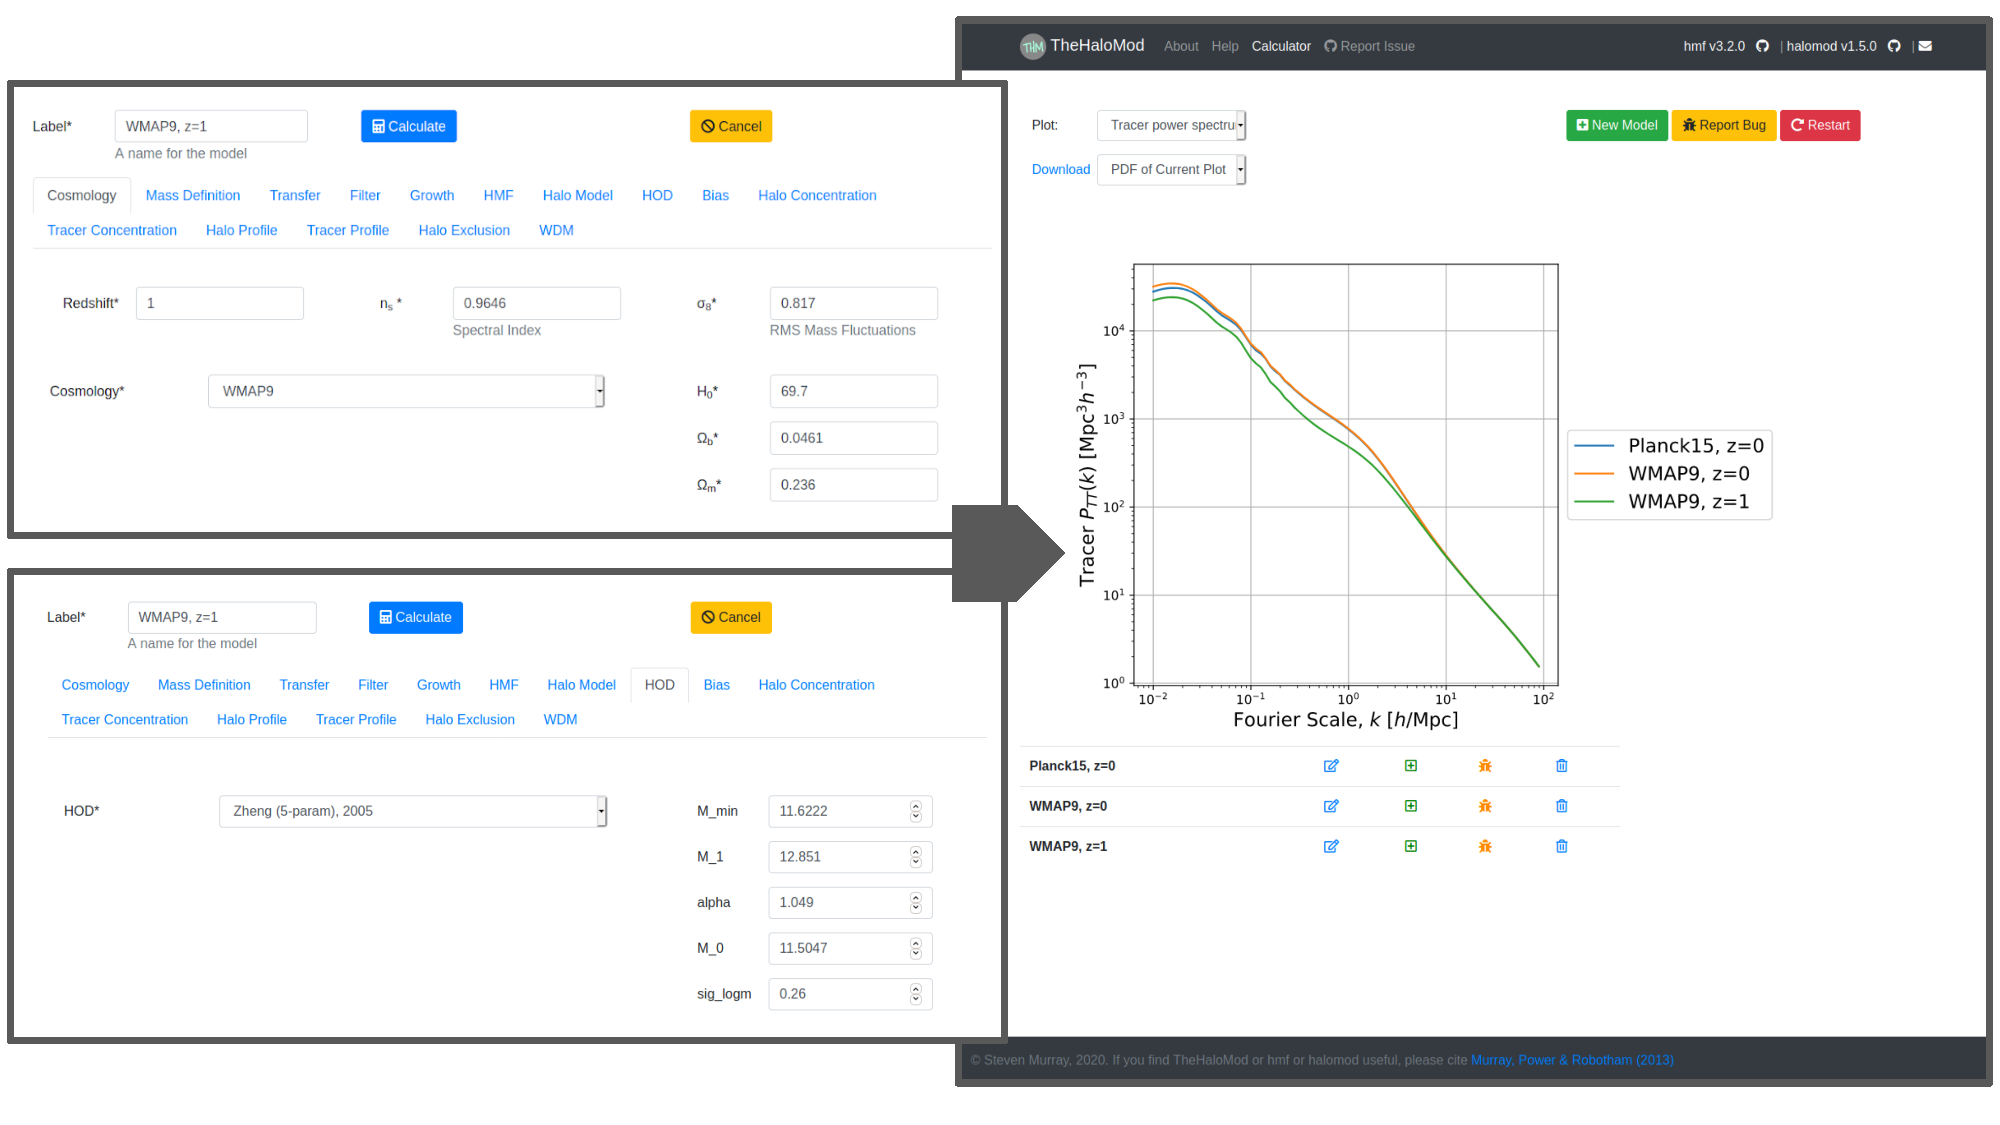
\includegraphics[width=\linewidth]{figures/thehalomod_app_schematic.pdf} 
    \caption{\textsc{TheHaloMod} in action. The main page (right panel) shows the currently computed models, with a selection of quantities to plot, and a number of actions available for each model (edit/clone/report bug/delete). The input form (two insets on the left) provides a wide range of options, including all of the components presented throughout this paper. Each component is defined in its own tab. Those shown here are cosmology and the HOD model.} \label{fig:webpage-image}
\end{figure*}

This paper is structured as follows: \S\ref{sec:DMHaloModel} details the theory of the HM particularly in the context of dark matter two-point statistics, collating the various components involved in a manner consistent with our implementation. Following this, we describe how to extend the halo model to tracer populations in \S\ref{sec:TracerHaloModel}. Then, we describe our code and its usage in  \S\ref{sec:halomod}, and in \S\ref{sec:applications} we present an illustrative example. In \S\ref{sec:future} we define a prospectus for the future, before summarising and concluding in \S\ref{sec:summary}.

Note that the code to produce all figures of different component models in this paper, as well as the example application, are available publicly as examples in \halomod's documentation\footnote{At \url{https://halomod.readthedocs.io/en/latest/examples/component-showcase.html} and \url{https://halomod.readthedocs.io/en/latest/examples/fitting.html} respectively.}. This paper refers to \textsc{hmf} version 3.2.1 and \textsc{halomod} version 2.0.0.


\section{The Dark Matter Halo Model}
\label{sec:DMHaloModel}
The broad assumption underpinning the HM is that in hierarchical structure formation scenarios, all mass is expected to be bound to halos at some scale\footnote{This assumption is clearly an approximation, since even cold dark matter (CDM) has a free-streaming scale in the early Universe below which we expect non-virialized mass \citep{Frenk2012,Schneider2014a}}. If this is the case, then the entire nonlinear density field may be reconstructed by summing contributions from the individual halos. If, in addition, we may describe the average radial density profile of halos as spherically-symmetric, with a shape that depends solely on the mass of the halo itself, we can write:
\begin{equation}
    \label{eq:hm_sum}
    \rho(\mathbf{x}) = \sum \rho_{h,i}(|\mathbf{x} - \mathbf{x_i}|,m_i)
\end{equation}
where $\rho_{h}(r|m)$ is the density of a halo with mass $m$ at radius $r$, and $x_i$ are the coordinates of the halo centres. 

The application of the HM rests in converting the prem\-ise of Eq. \ref{eq:hm_sum} into a semi-analytic integration. This requires knowledge of four key components:
\begin{enumerate}
    \item The average radial density profile of halos, $\rho(r|m)$
    \item The abundance of halos of a given mass (termed the halo mass function, or HMF), $n(m)$
    \item The expected overdensity of halos of mass $m$, $\delta_h(\mathbf{x},m)$ in a region with a given overdensity of matter $\delta(\mathbf{x})$, called the \textit{halo bias}.
    \item A model for the linear spatial distribution of matter, $\delta(\mathbf{x})$.
\end{enumerate}
Furthermore, detailed calculations require the following extra components:
\begin{enumerate}
    \setcounter{enumi}{3}
    \item Additional parameters that describe the halo profile, most
    commonly parameterized as a concentration-mass relation, $c(m)$, linking the shape of a halo profile to its mass.
    \item A model for ``halo exclusion", which accounts for double-counting intra-halo correlations.
    \item To extend the calculations to galaxies, a distribution function for the occupation of halos by galaxies, as a function of halo mass, $N(m)$ (the HOD; cf. \S\ref{sec:TracerHaloModel}). 
\end{enumerate}

Although the halo model can be used to describe the density field at any level of the $n$-point hierarchy, its most common application to date has been to compute two-point statistics. Thus, in this outline, we shall focus on the framework as it pertains to the 2PCF.

Our aim in this section is to introduce the theory in a manner conducive to our implementation, so we shall cover each of the six components in turn following the presentation of the core framework.


Throughout the section, we discuss isotropic two-point statistics, which measure the over-density of pairs of points at a certain scalar separation. This can be formulated either in Euclidean space, as the correlation function $\xi(r)$, or in Fourier-space, as the power spectrum $P(k)$. 
The correlation function is defined as the excess probability of locating a particle at separation $\mathbf{r}$ from a particle at position $\mathbf{x}$ in a given spatial distribution, and is written (for a homogeneous universe)
\begin{equation}
    \xi(\mathbf{r}) = \frac{1}{V}\int_V d^3\mathbf{x}\ \delta(\mathbf{x}) \delta(\mathbf{x} - \mathbf{r}),
\end{equation}
where $\delta(\mathbf{x})$ is the overdensity
\begin{equation}
    \delta(\mathbf{x}) = \frac{\rho(\mathbf{x}) - \bar{\rho}}{\bar{\rho}}.
\end{equation}
The power spectrum is merely the Fourier transform of the correlation function, and the standard Fourier convention in cosmology renders it
\begin{equation}
    \xi(\mathbf{r}) = \int \frac{d^3 \mathbf{k}}{(2\pi)^3} P(\mathbf{k}) e^{i \mathbf{k}\cdot \mathbf{r}}.
\end{equation}
Under the assumption of cosmic isotropy, the correlation function and power spectrum depend only on the amplitude of $\mathbf{r}$ and $\mathbf{k}$, respectively. Transformation from an (isotropic) power spectrum $P(k)$ to an (isotropic) correlation function $\xi(r)$ can thus be performed using an order-$1/2$ \textit{Hankel} transform, which is the 3D Fourier transform of a spherically symmetric distribution:
\begin{equation}
\label{eq:hankel}
\xi(r) = \frac{1}{2\pi^2}\int_0^\infty P(k)k^2 j_0(kr)dk,
\end{equation}
where $j_0$ is the zeroth-order \textit{spherical} Bessel function,
\begin{equation}
    j_0(x) = \frac{\sin x}{x}.
\end{equation}
We note that the halo model is \textit{not limited} to such two-point statistics, but our implementation currently is.

\subsection{Clustering Framework}
\label{sec:haloclustering}
It is convenient to formulate the framework of clustering in two regimes \citep{Seljak2000}, intra- and inter-halo pairs, called the 1-halo and 2-halo terms respectively. These approximately correspond to small- and large-scale structure (i.e. the contribution of each in the opposite regime is negligible), where `small' is sub-megaparsec, and `large' is $>\sim5h^{-1}$Mpc. 

Throughout the following, the superscripts $1h$ and $2h$ will be used to denote this segregation. Furthermore, a subscript of $DM$ will denote a dark matter statistic, while $T$ will denote statistics of observable tracers (such as optical or HI-selected galaxies). 

The total power spectrum and 2-point correlation function can be written simply as
\begin{equation}
    P(k) = P^{1h}(k) + P^{2h}(k),
\end{equation}
and
\begin{equation}
    \xi(r) = [1 + \xi^{1h}(r)] + \xi^{2h}(r).
\end{equation}
We will first describe the calculation of the 1-halo and 2-halo terms, each of which combines multiple physical components, which we will proceed to describe in 
\S\ref{sec:powerspec}-\ref{sec:theory:exclusion}.

\subsubsection{1-halo term}
The pair-counts, proportional to $1+\xi$, within a halo of mass $m$, are given by the self-convolution of the halo profile. Thus the total pair counts, normalised by a random field (specified by the constant $\bar{\rho}^2$) is given by
\begin{equation}
\label{eq:dmcorr1}
1 + \xi_{DM}^{1h}(r) = \int n(m) \left(\frac{m}{\bar{\rho}}\right)^2 \lambda(r|m) dm,
\end{equation}
where $\lambda$ is the mass-normalised self-convolution (i.e. the 3D integral of the profile multiplied by itself after a shift of length $r$, cf. \S\ref{sec:profilestheory}), and $n(m)$ is the halo mass function (HMF).

It is common to express this in Fourier-space, since the self-convolution becomes a simple multiplication,
\begin{equation}
    \label{eq:dmpower1}
    P_{DM}^{1h}(k) = \int n(m) \left(\frac{m}{\bar{\rho}}\right)^2 |u(k|m)|^2 dm,
\end{equation} 
where $u(k|m)$ is the normalised Fourier transform of the halo profile. This form has the distinct advantage that higher-order correlations merely involve an increase in the exponent of $u$, rather than an intractable multi-dimensional convolution. Conversely, for numerical purposes, if an analytic formulation of the self-convolution exists and the intended quantity is the correlation function, then it is more efficient to use Eq. \ref{eq:dmcorr1} directly. 

\subsubsection{2-halo term}
\label{sec:theory:2halo}
The two-halo term is most elegantly expressed in Fourier-space, 
\begin{align}
    P_{\rm DM}^{2h}(k,r) =  \int \int & dm_1 dm_2\  I_{\rm DM}(k,m_1) I_{\rm DM}(k,m_2) \nonumber \\ 
    &\times P_{hh}(k,r|m_1,m_2),
\end{align}
where
\begin{equation}
    I_{\rm DM}(k,m) = n(m) u(k|m) \frac{m}{\bar{\rho}}.
\end{equation}
Here, $P_{hh}(k,r|m_1,m_2)$ is the power spectrum of halo centres for halos of mass $m_1$ and $m_2$. This is in general a complicated function of mass and scale, but the most common approach is to approximate it by a first-order linear bias of the matter power,
\begin{equation}
    \label{eq:halo_centre_power}
    P_{hh}(k,r|m_1,m_2) \approx b(m_1,r)b(m_2,r)P_m(k),
\end{equation}
where $b(m,r)$ is the first-order bias at $m$ (cf. \S\ref{sec:biastheory}), possibly with a scale-dependent correction, and $P_m(k)$ is the matter power spectrum (cf. \S\ref{sec:powerspec})\footnote{Note that thoughout, we use a subscript $m$ to denote either the linear matter power or the nonlinear matter power derived using analytic corrections, as opposed to the full halo model.}. Typically, empirical nonlinear corrections on the linear matter power spectrum from \textsc{halofit} \citep{Smith2003} are used for this quantity. We leave its definition free in our implementation\footnote{This is slightly circular, as the \textsc{halofit} model itself uses the halo model. However, this is a common practice in halo model calculations, eg. \citep{Cooray2002, Smith2011}}.

The general form for the 2-halo term then becomes
\begin{align}
\label{eq:dmpower2a}
    P_{\rm DM}^{2h}(k,r) =  \int\int & I_{\rm DM}(k,m_1) I_{\rm DM}(k,m_2) \nonumber \\
    &\times b(m_1,r)b(m_2,r)P_{m}(k) dm_2 dm_1
\end{align}
This is separable, so long as the integration limits are not inter-dependent (this is not the case in general, cf. \S\ref{sec:theory:exclusion}), and in this simplest case (where we do not attempt to exclude correlations within halos) we have
\begin{equation}
    \label{eq:dmpower2}
    P_{DM}^{2h}(k,r) = P_m(k) \left[ \int  I_\text{DM}(k,m) b(m,r) dm \right]^2.
\end{equation}

Note that all of these expressions denote the 2-halo term as a function of both $k$ and $r$ (as opposed to the 1-halo term which is just a function of $k$). 
This arises either due to the appropriate limits of the integration being dependent on the real-space size of halos, or because the halo bias may be scale-dependent. 
In cases when either of these is true, to recover the power spectrum as a function of $k$ only, we Hankel-transform to $\xi(r)$ and then back to $P(k)$.


\subsection{Matter Power Spectrum}
\label{sec:powerspec}
The matter power spectrum $P_m(k)$ characterises the distribution of matter 
density perturbations as a function of wavenumber $k$.
When density fluctuations are small, so that $\delta \ll 1$, the statistical properties of the perturbations can be derived analytically via perturbation theory. 
Generally, it is assumed that the fluctuation spectrum was initially scale-free (i.e. a power-law), and the present day (linear) power spectrum is modified by a transfer function which captures the effects of the transition from a radiation-dominated to matter-dominated Universe \citep{Bond1984}:
\begin{equation}
	\label{eq:powerfromtransfer}
	P_\text{m,lin}(k) = Ak^n T^2(k),
\end{equation}
where $A$ is the normalisation constant and $n$ is the spectral index. 
We follow convention and use the
parameter $\sigma_8$, which measures the mass variance on a scale of $8 h^{-1}$Mpc at $z=0$, 
to calculate $A$. The transfer function is particularly sensitive to the nature of
the dark matter and the baryon density parameter $\Omega_\text{b}$.

A commonly used dimensionless equivalent can be defined as 
\begin{equation}
    \Delta^2(k) = \frac{k^3}{2\pi^2} P(k),
\end{equation}
which is the contribution to the variance in logarithmic wavenumber bins.

The CDM transfer function has been modelled extensively in the literature. 
A number of functional forms have been proposed \citep[][hereafter EH]{Bond1984,Bardeen1986,Eisenstein1998}, along with a series of \textit{Boltzmann} codes, which calculate the transfer function from first principles with perturbation theory techniques \citep{Zaldarriaga2000,Lewis2000,Blas2011}. 

Figure \ref{fig:power} shows the typical shape of the CDM linear power spectrum, while highlighting differences between forms for $T(k)$ found in the literature. Both small- and large-scales have small fluctuations, with a characteristic turnover at scales of $\sim 0.02h/$Mpc. The low-$k$ form asymptotes to $P(k \ll 0.02 ) \propto k^{n_s}$, while the high-$k$ behaviour is more complicated, not obeying a power-law relation. Only the Boltzmann code is able to fully capture the wiggles introduced by the baryon acoustic oscillations (BAOs), though the EH form including baryons closely follows up to $k \sim 2 h^{-1}{\rm Mpc}$. 
In fact, all curves (except that of \citet{Bond1984}) are within $\sim 10\%$ over the plotted range.

\begin{figure}
  \centering
  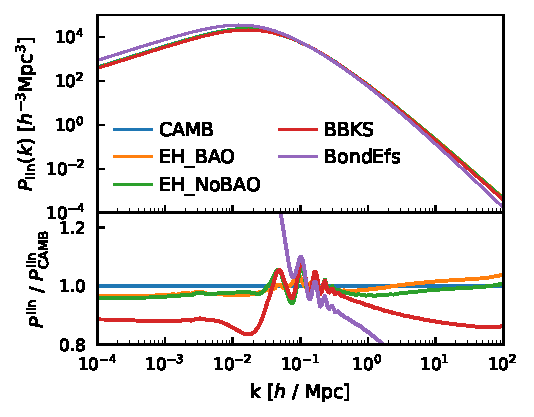
\includegraphics[width=\linewidth]{figures/transfer_models.pdf}
  \caption[Comparison of transfer function models]{A selection of transfer function models, shown as linear power spectra, including analytic approximations \citep{Bond1984,Bardeen1986,Eisenstein1998} and Boltzmann solutions. Details for each model (referenced to the alias given in the legend) can be found in Table \ref{tab:models_transfer}. The general shape is reproduced in each case, with details of baryon acoustic oscillations differing. In the bottom panel, we show the relative fraction compared to the CAMB transfer function, which renders all models without baryons as having oscillations on the acoustic scales.}
  \label{fig:power}
\end{figure}
  
The calculation of the halo-centre power spectrum is commonly approximated by Eq. \ref{eq:halo_centre_power}, i.e.
\begin{equation*}
    P_{hh}(k,r|m_1,m_2) \approx b(m_1,r)b(m_2,r)P_m(k),
\end{equation*}
 in which an estimate of the matter power spectrum is linearly biased. Typically, a \textit{nonlinear} estimate of the matter power is used, for which the corrections of \citet[][hereafter \textsc{halofit}]{Smith2003} are employed. We do not present the details here, except to mention that the modifications are applied as ratios of $P_\text{m,lin}(k)$, which are obtained via arguments motivated by the halo model. These modifications are expressed as a series of equations with coefficients fitted to numerical simulations. Updated coefficients were introduced in \citet{Takahashi2012}. Note also that the normalisation of $P_\text{m,nl}(k)$ is ident\-ical to $P_\text{m,lin}(k)$, and is calculated using the linear form, since $\sigma_8$ refers to the linear power spectrum. The effect of introducing non-linearities is to increase small-scale power, with the recent coefficient updates slightly enhancing this effect.

\subsection{Mass Definition}
\label{sec:theory:massdef}
The halo model centres on the `halo' as its basic unit.
One of the most fundamental properties of the halo is its mass, which is required to define the density profile, concentration-mass relation and its bias with respect to background matter, but there is no unique way in which to define this property. 
%This ambiguity arises as the consequence of being unable to prescribe a uniquely meaningful boundary to the halo, which exists as a semi-amorphous collection of particles, and many definitions have arisen. \bd{I'd remove this sentence, it'll only annoy people. For example, peope such as myself would argue that there is a well-defined boundary, it's just hard to properly identify numerically}

The two dominant approaches to defining the halo mass are the \textit{Friends-of-Friends} (FOF) and \textit{Spherical Overdensity} (SO) definitions. 
The FOF definition is useful in the context of simulations, in which we have known particle locations. These particles are linked together into a halo if their separation is less than some chosen linking length, and the fully linked network provides a halo of arbitrary shape.

The SO algorithm finds peaks in the density field and grows spheres around them until the contained density drops below a threshold density.
All particles within the final sphere are considered part of the halo. 
This definition is more useful in the context of observations (of clusters, for example) as it can be applied to the measured (projected) density fields\footnote{Note that the 3D SO definition is not \textit{immediately} applicable to observations without forward-modelling and scaling relations, but they are far more applicable than FoF masses.}. 

Within each definition approach exists the potential for an infinite number of explicit definitions. The FOF approach has the linking length parameter (typically denoted $b$), whilst the SO approach has the overdensity threshold, $\Delta_h$. Moreover, the conversion between FOF and SO masses is difficult because a linking length does not uniquely correspond to an overdensity \citep{More2011}.

While it is thus difficult to compare, even in principle, between FOF and SO definitions, comparison of halo model quantities between explicit SO definitions is possible (to first order) as long as one has a model for the density distribution within a halo (cf. \S\ref{sec:halomod:components:profile}).
Armed with an average spherical halo profile, one can compute the average mass of a halo under a different density threshold (clearly higher density thresholds resulting in lower masses) (cf. \S\ref{sec:halomod:components:mass-def}). 
We will use the standard symbols $m$ and $R$ for the halo mass and radius throughout this paper, typically without specifying which definition is being applied (most equations are agnostic of this definition). 


\subsection{Variance and Spatial Filter}
\label{sec:theory:filter}
The halo model depends on knowing the overdensity (and variance) associated with a position $\vec{x}$. 
The mass variance is defined over some smoothing scale, $R_L$:
\begin{equation}
	\label{eq:massvariance}
	\sigma^2(R_L(m)) = \frac{1}{2\pi^2}\int_0^\infty{k^2P_{\rm m, lin}(k)W^2(kR)dk}.
\end{equation}

$W(x)$ here denotes a spatial filter.
In particular, halos arise from patches in the primordial density field with some shape, described by a function $w(\mathbf{x})$.
While the shape of the filter may be arbitrary (and should be matched to the typical shapes of the primordial patches that give rise to the halos \citep{Dalal2010, Chan2017,Diemer2019}), the most common choices are a spherical top-hat (either in real or Fourier space) or a Gaussian.
Under the assumption that the chosen filter is spherically symmetric (not the case in general, but assumed in \halomod), the Fourier-transform of the filter is given by the spherical-hankel transform:
\begin{equation}
    W(k) = 4\pi \int_0^\infty w(r) r^2 j_0(kr) dr.
\end{equation}

Having defined a spatial filter on the primordial density field, one can proceed to define the Lagrangian radius, $R(m)$, which is the radius of a spherical region of homogeneous space containing the mass $m$ (or more generally, the scale of a particular filter function required to contain the mass, cf. \S\ref{sec:halomod:components:window}). For the standard top-hat, this is
\begin{equation}
    R_L(m) = \left(\frac{3m}{4\pi\bar{\rho}_0}\right)^{1 / 3},
\end{equation}
with $\bar{\rho}_0$ the mean density of the Universe at the present epoch.

The ``mass variance'', $\sigma^2(R_L)$ is thus the variance on a scale from which the matter in halos is thought to have originated. Notably, the mass variance in spheres of Lagrangian radius 8 Mpc/$h$ yields the power spectrum normalisation, $\sigma_8$.

\subsection{Mass Function}
\label{sec:massfunction}
The mass function quantifies the number of dark matter halos per unit
mass per unit comoving volume of the Universe. 
%We do not include a detailed summary of the theory of the mass function here, and direct the reader to \citet{Murray2013a} for a review and table of fitting functions. 
The most commonly adopted theoretical formulation of the mass function is via the extended Press-Schechter (EPS) formalism \citep{Press1974,Bond1991}, in which density peaks form through gravitational instability and evolve into halos when they cross a density threshold, $\delta_c$. 
In this formalism, the mass function is a universal function of the peak-height, $\nu = \delta_c/\sigma$\footnote{Note that some authors use $\nu = \delta^2_c/\sigma^2(m)$, i.e. the square of our definition.}, which captures the variation from cosmological parameters and the redshift \citep[but note that several recent studies find significant non-universality with redshift, and have provided fits that explicitly account for this departure]{Jenkins2001}. 

The mass function can be defined as
\begin{equation}
\label{eq:hmf}
  n(m) \equiv \frac{dn}{dm} = \frac{\rho_0}{m^2} f(\sigma) \left|\frac{d\ln\sigma}{d\ln m}\right|,
\end{equation}
or using the peak-height, as
\begin{equation}
    \label{eq:theory:hmf_nu}
    \frac{dn}{dm} = \frac{\rho_0}{m} f(\nu) \frac{d \nu}{d m}.
\end{equation}

For an Einstein-de Sitter universe (in which the matter density equals the critical density and there is no dark energy), $\delta_c \approx 1.686$, and its value is very weakly dependent on cosmology\footnote{Note that even small changes in $\delta_c$ can affect the high-mass end of the HMF significantly. However, many authors assume $\delta_c = 1.686$ regardless of cosmology and thus many fits of the HMF are defined under this assumption.}
The function $f(\sigma) \equiv \nu f(\nu)$, denoting the fraction of matter collapsed into halos of peak-height in a logarithmic bin around $\nu$, has been modelled extensively in the literature, and is generally fit to numerical simulations\footnote{Note that some authors use $f(\nu)$ to describe what we have defined as $\nu f(\nu)$.}. 

It can be advantageous (but not strictly necessary) to choose a fitting function which is normalisable, ie.
\begin{equation}
    \label{eq:fnu1}
    \int f(\nu) d\nu = 1.
\end{equation}
Several fits in the literature obey this relation \citep[eg.][]{Sheth2001,Peacock2007,Tinker2010},  which ensures that all mass is bound in halos. This is particularly attractive for HM calculations, in which it is consistent with the basic assumptions of the framework.

Note also that from Eq. \ref{eq:theory:hmf_nu} we can determine $d\nu$ as a function of $dm$, and integrals of the form $\int n(m) g(m) dm$ may be re-written
\begin{equation}
    \label{eq:integrate_over_nu}
    \int g(\nu(m)) \frac{\rho_0}{m} f(\nu) d\nu.
\end{equation}
In particular, the sum of all mass in the universe requires setting $g(m) = m$, and the requirement that the mass density in halos equal $\rho_0$ is easily seen to be equivalent to the condition Eq. \ref{eq:fnu1}. 
Integrating Eq. \ref{eq:integrate_over_nu} can often be numerically advantageous, since relevant bounds on $f(\nu)$ can often be found independently of cosmology and redshift.

Figure \ref{fig:mfs} shows the HMF for four of the fits available in \textsc{halomod} (via \textsc{hmf}). According to these fitting functions, the HMF behaves as a power-law at low masses, with an exponential cut-off above a typical mass $m_* \approx 5\times10^{14}$ (this mass changes with redshift). There is clearly significant variations between the fits, especially at high masses, for a range of reasons, including halo finder differences, alternate mass definitions, and simulation resolution \citep[cf.][]{Murray2013a,Knebe2011}. 

\begin{figure}
  \centering
  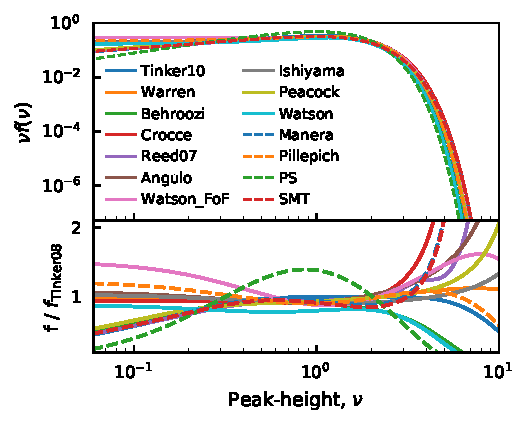
\includegraphics[width=\linewidth]{figures/hmf_models.pdf}
  \caption[Several HMF fits]{Seven HMFs from the literature, including the `original' form of \protect\citet[][`PS']{Press1974}, motivated by spherical collapse, and \textsc{SMT} motivated by ellipsoidal collapse from \protect\citet{Sheth2001}).}
  \label{fig:mfs}
\end{figure}


%However, as seen in Figure \ref{fig:mf_fit_corr}, these variations are not as pronounced in the resulting $\xi_{gg}(r)$, \bd{Don't think we've even defined the galaxy-galaxy correlation?? Maybe this figure is premature at this point in the paper.} due to integration with the variation occurring at small values. The two-halo term is modified by a near-constant factor dependent primarily on the amplitude of $n(m_*)$. The one-halo term has a more complicated dependency. 


% \begin{figure}
%   \centering
%   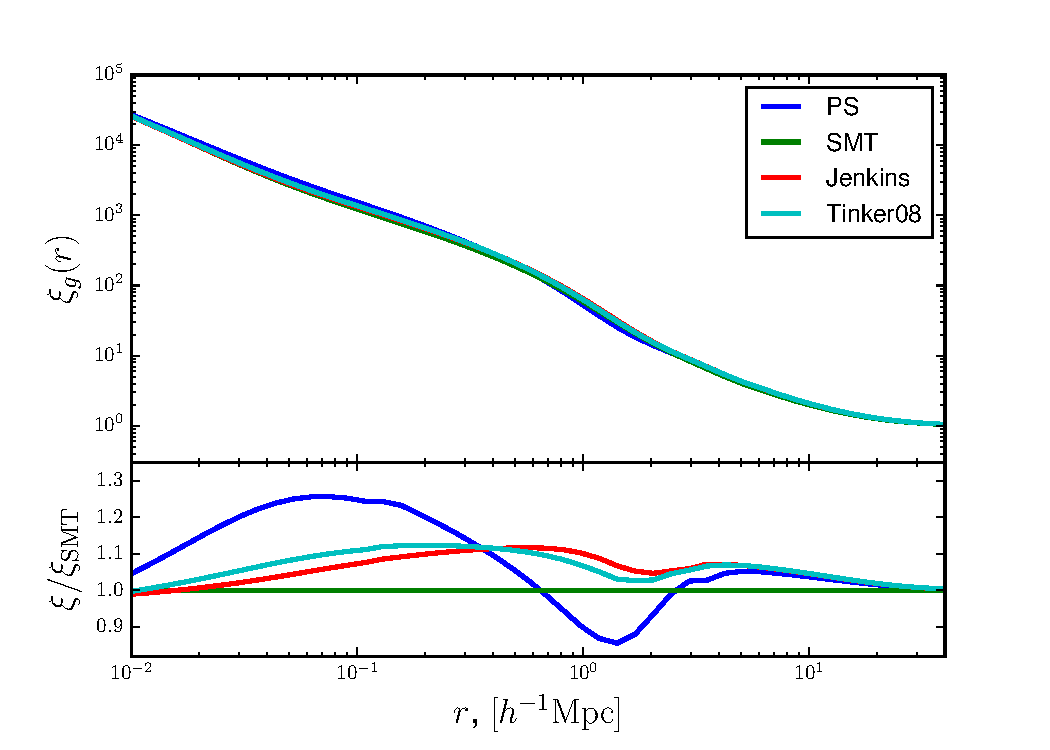
\includegraphics[width=\linewidth]{figures/corr_mffits.pdf}
%   \caption[Effect of the HMF fit on the two-point correlation function]{Effect of the varying HMF fits on the two-point correlation function, where the mean galaxy density is matched in each case by shifting the HOD parameter $M_\text{min}$, where $M_\text{min} = 10^{11}h^{-1}M_\odot$ for the SMT function. The variation is reduced to $<10$\% for fits other than PS.}
%   \label{fig:mf_fit_corr}
% \end{figure}


\subsection{Bias}
\label{sec:biastheory}
It is well-known that dark matter halos tend to trace the underlying density field in a biased manner \citep[eg.]{Cole1989}. In principal, the form of this bias can be of arbitrary order (as a function of the matter overdensity), non-local (i.e. dependent on the surrounding environment) and stochastic. However, it is most common within studies involving the halo model to consider only the first-order, local, deterministic bias as a function of the halo mass \citep{Mo1996}: 
\begin{equation}
    \delta_h(\bar{x},m) = b(m) \delta(\bar{x}).
\end{equation}

Peaks theory is able to make predictions of the form of $b(m)$, by considering the probability of collapse of a region of given smoothing scale $m$ in the context of an altered density threshold $\delta_c - \delta(\vec{x})$, often called the peak-background split method \citep[for more details, see eg.][]{Bond1991,Zentner2007,Tinker2010,Manera2010}. These predictions are specified in terms of the peak-height parameter $\nu$, and are therefore expected to exhibit universality with respect to cosmology and redshift.

In the spherical collapse paradigm, the bias is intimately related to the mass function \citep{Cole1989,Cooray2002}, 
\begin{equation}
    b(m) = 1 - \frac{\partial}{\partial \delta_c} \ln n(m),
\end{equation}
which when combined with Eq. \ref{eq:hmf}, gives
\begin{equation}
    b(m) = 1 - \frac{1}{\delta_c} - \frac{\partial}{\partial \delta_c} \ln f(\nu).
\end{equation}
In this formalism, if all mass is contained within halos, according to Eq. \ref{eq:fnu1}, then by construction, the following consistency relation holds,
\begin{equation}
\label{eq:consistency}
    \int b(\nu) f(\nu) d\nu = 1, 
\end{equation}
which merely says that the average bias is unity, so that matter is not biased against itself\footnote{Non-unity average bias in the context of the halo model would be an inconsistency, as all halos contain all the mass, and the mass cannot be biased, on average, against itself.}. 

In the approximation of spherical collapse, under the original model of \citep{Press1974}, we have $f(\nu) \propto \exp(-\nu^2/2)$, which yields a bias of  \citep{Cole1989,Mo1996}
\begin{equation}
    b(\nu) = 1+ \frac{\nu -1}{\delta_c}.
\end{equation}
The general qualities of the spherical collapse form are (recall that $\nu = 1$ at $M_\star \sim 5\times10^{12}$ at $z=0$, and corresponds the mass of halos that are, on average, collapsing at a given redshift): 
\begin{itemize}
    \item  a transition from low-mass anti-bias to high-mass bias at $\nu = 1$
    \item a small-scale asymptotic limit of $b = 1 - 1/\delta_c \approx 0.4$
    \item a large scale asymptotic behaviour of $b \propto \nu$. 
\end{itemize}

Given the simplistic nature of the spherical collapse model, it is remarkable that this bias function roughly reproduces the results of $N$-body simulations. However, in detail, this form over-predicts the bias at high masses ($\nu >\sim1.5$), and consequently slightly under-predicts the bias for low-mass halos. 

The approximations induced by the spherical collapse assumption have been relaxed in several studies, most notably by \citet{Sheth2001}, who obtain a form motivated by ellipsoidal collapse, but calibrated with simulations. Forms motivated by stochastic barriers \citep{Corasaniti2011}, non-Markovian barriers \citep{Ma2011} and local density-maxima \citep{Paranjape2013a} are more recent developments.

Unfortunately, the spherical collapse paradigm leads to an artificial enhancement of the bias for halos with $\nu < \sim 1$ \citep{Manera2010,Tinker2010}, due to the fact that low-mass halos are increasingly elliptical. This has resulted in a proliferation of direct empirical fits to high-resolution $N$-body simulations \citep{Jing1998,Jing1999,Seljak2004,Tinker2005,Mandelbaum2005,Pillepich2010}.
Motivated by the broad success of spherical collapse, these fits are usually \citep[but see][]{Jing1998,Seljak2004} still formulated in terms of the peak-height (indeed, often they utilise the forms yielded by the peak-background split, with updated parameters based on direct fits to simulations).

In figure \ref{fig:bias_functions} we show a sample of linear scale-independent bias relations found in the literature and included in \halomod. We note the similarity of high-mass behaviour, though the high-mass amplitude is substantially modified between several of the forms. 

\begin{figure}
  \centering
  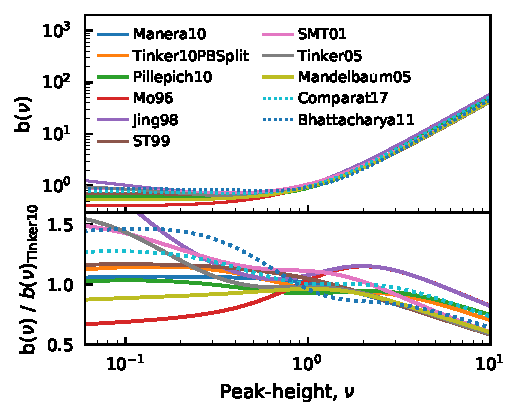
\includegraphics[width=\linewidth]{figures/bias_models.pdf}
  \caption[Several bias functions from the literature]{Several linear bias functions from the literature.Most functions, including \protect\citet{Mo1996}, \protect\citet{Sheth1999}, \protect\citet{Sheth2001} and those with the same form \protect\citep{Mandelbaum2005,Tinker2005} have high-mass asymptotic behaviour of $b \propto \nu$. The (default) form of \protect\citet{Tinker2010} is an empirical fit with an arbitrarily chosen form, and has a high-mass asymptotic limit of $b \propto  \nu^{1.2}$. The models plotted in dotted lines are from \textsc{colossus}, called by \halomod\ using its explicit interface}
  \label{fig:bias_functions}
\end{figure}

\subsubsection{Scale-dependence}
\label{sec:theory:bias:sd}
In reality, the assumption that the bias is a function only of halo mass, to the exclusion of environment, is overly simplistic \citep{Sunayama2015}. 
The bias depends not only on the masses of the paired halos, but also the scale over which we consider the correlations. 
The scale-dependence of halo bias is a complex phenomenon, which has received a great deal of attention \citep[eg.][]{Paranjape2013,Lapi2014,Poole2015}. Foregoing these complexities, simple empirical models specify the scale-dependence as a function $S(\xi_m(r))$,
\begin{equation}
    b^2(m,r) = b^2(m) S(\xi_m(r)).
\end{equation}
An example form for $S$ is given by \citet{Tinker2005} as
\begin{equation}
	\label{eq:sdb}
	S(r) = \frac{\left[1+1.17\xi_m(r)\right]^{1.49}}{\left[1+0.69\xi_m(r)\right]^{2.09}}.
\end{equation}
At large scales, where $\xi \ll 1$, the scale-dependence is negligible, but smaller scales can receive significant ($\sim 50\%$) suppression. 


% Later \citet{seljak2004} give a bias relation as 
% \begin{equation}
%  b(x) = 0.53 + 0.39x^{0.45} + \frac{0.13}{40x+1}+5\times10^{-4}x^{1.5}
% \end{equation}
% which they extend to be cosmologically dependent as
% \begin{equation}
%  b_c(x) = b(x) + \log_{10}(x)[0.4(\Omega_M - 0.3 + n_s -1)+0.3(\sigma_8-0.9+h-0.7)+0.8\alpha_s].
% \end{equation}
% Here $x$ is the ratio of mass to the non-linear mass $m_*$, which is defined by $\sigma(m_*) = \delta_c$. \citet{tinker2005} found that due to its dependence on $m/m_*$ rather than the conventional $\nu$, this fit was not accurate in a universal sense -- only close to the concordance model. They thus provide an extended fit motivated by the Sheth-Tormen mass function





\subsection{Halo Density Profiles}
\label{sec:profilestheory}
It is widely accepted that the density profiles of DM halos are more or less self-similar if they are rescaled by a suitable central density and radial scale. These two parameters can then be expressed more intuitively as a mass and a concentration. In this section, we define our nomenclature for density profiles. Our general, systematic formulation enables the user to elegantly insert specific functional forms. In particular, the average density profile follows the form
\begin{equation}
    \label{eq:universalprofile}
    \rho(r|m,z) = \rho_s(c, \bar{\rho}) \times f(r/r_s),
\end{equation}
where $\rho(r|m,z)$ has units of density, and $c(m,z) = r_{\Delta_h} / r_s$ is the \textit{concentration parameter}, which we shall treat as an explicit function of the halo mass, redshift, and cosmology (although it exhibits appreciable scatter around any such relationship). Here, $\bar{\rho}$ is the mean matter density of the universe at redshift $z$.  The \textit{scale radius} $r_s$ is often defined as the radius where the logarithmic slope of the profile is $-2$, but other definitions are possible in principle. The factor $\rho_s$ controls the amplitude of the profile and is set by the known mass given the halo's radius (here we use halo radius generically as $r_{\Delta_h}$, where $\Delta_h$ is the halo overdensity with respect to the background). In particular, it is always true that the halo radius and mass are related by
\begin{equation}
    \label{eq:mass-radius-halo}
    m = \frac{4\pi r^3_{\Delta_h}}{3} \bar{\rho} \Delta_h.
\end{equation}
We may consider halos to have either a `hard' or `soft' edge; in the former case, the extent of the halo is precisely at $r_{\Delta_h}$, and the density abruptly falls to zero beyond this. In the latter case, the halo extends to infinity. The latter case is only well-defined in the case that the total integrated mass converges. The HM generally considers halos with a hard boundary, but \halomod\ includes models for both, and we will present the equations for `non-truncated' halos as well.

While $\rho_s$ does not directly depend on mass in our formulation, the dependence on the mean density and the secondary dependence of $c$ on mass translate into a relation where more massive and earlier-forming halos have higher central densities. The $f(r/r_s)$ term controls the shape of the profile and is a function of the scaled radius $x=r/r_s$. Throughout the following discussion we shall often refer to a `reduced' form of the profile (or related quantities) in which simple normalisation factors are removed. An example of such a reduced form is $f$ in Eq. \ref{eq:universalprofile}.

% and at this stage only considers profiles with two parameters (one of which is set by the halo overdensity $\Delta_h$, and the other we label as ``concentration"). Multi-parameter profiles \citep[eg. the `Einasto' profile,][]{Navarro2004} will be left for future versions.

\subsubsection{Truncated Halos}
For halos truncated at the halo radius, the amplitude of the profile is set by the total mass inside the halo radius, which we recover by integrating Eq. \ref{eq:universalprofile}:
\begin{equation}
\label{eq:minrv}
m = 4\pi \rho_s(c) r_s^3 \int_0^c x^2 f(x) dx,
\end{equation}
where we have made the substitution $r = xr_s$ in which $x(r_{\Delta_h}) = c$.
If we set
\begin{equation}
\label{eq:hofc}
h(c) = \int_0^c x^2 f(x) dx
\end{equation}
then we obtain
\begin{equation}
\label{eq:hofm}
\rho_s(c) = \frac{m}{4 \pi r_s^3 h(c)} \equiv \frac{c^3 \Delta_h}{3h(c)}\bar{\rho}
\end{equation}
Thus for all profiles, $h(c)$ uniquely defines the amplitude.

The calculation of two-point statistics involves two more functions derived from the halo density profile: the normalised Fourier transform $u(k|m,z)$ and the self-convolution $\lambda(r|m,z)$. The normalised Fourier transform of the halo profile is defined as \citep{Cooray2002}
\begin{equation}
\label{eq:ugeneral}
u(\mathbf{k}|m,z) = \frac{1}{m}\int \rho(\mathbf{r}|m,z) e^{-i\mathbf{r}\cdot\mathbf{k}}d^3\mathbf{r}
\end{equation}
in which $\mathbf{k},\mathbf{r}$ are the Cartesian wave-vector and position vector respectively.
In the case of a spherically symmetric distribution truncated at the halo radius (as we assume) this may be treated by a Hankel transform, in which we use $\kappa = kr_s$, and $x$ as previously defined:
\begin{equation}
u(\kappa|m,z) = \frac{4\pi r_s^3}{m}\rho_s(c)\int_0^c x^2 \frac{sin(\kappa x)}{\kappa x}f(x) dx.
\end{equation}
Using Eq. \ref{eq:hofm} we have
\begin{equation}
\label{eq:uspherical}
u(\kappa |m,z) = \frac{p(\kappa,c)}{h(c)}
\end{equation}
where
\begin{equation}
\label{eq:pofck}
p(\kappa,c) = \int_0^c x^2 \frac{sin(\kappa x)}{\kappa x}f(x) dx
\end{equation}
is the reduced form.

%\begin{equation}
% \lambda(\mathbf{r}|m,z) = \int \rho(\mathbf{r'}|m,z)\rho(|\mathbf{r'}+\mathbf{r}||m,z)d^3\mathbf{r'}
%\end{equation}
The self-convolution of the density profile is
\begin{equation}
\label{eq:simplifiedlam}
 \lambda(x|m,z) = \rho_s^2(c) r_s^3 l(x,c)
\end{equation}
and has units of $M^2/V$. The reduced form is given by
\begin{equation}
\label{eq:lofxc}
l(x,c) = \int f(\mathbf{y},c)f(|\mathbf{y}+\mathbf{x}|,c)d^3y,
\end{equation}
in which $x$ and $y$ are in units of $r_s$ as usual. It is generally difficult, if not impossible, to solve this integral analytically. 
%However, following \citet{Ma2000}, for spherically-symmetric profiles we can write
%\begin{equation}
%    l(x,c) = \frac{2\pi}{x} \int
%\end{equation}
However, there are several profiles for which do afford a solution, including the popular profile of \citet[][hereafter NFW]{Navarro1997}.

Thus, any profile is fully defined by its reduced profile shape, $f(x)$, which can be used to produce the dimensionless quantities $h(c)$, $p(\kappa,c)$, and $l(x,c)$. We utilise this set of variables in the \verb|halomod| implementation. 

\subsubsection{Non-truncated Profiles}
In the case that the profile is not truncated at $r_{\Delta_h}$, we still define $c \equiv r_{\Delta_h}/r_s$, and assume Eq. \ref{eq:mass-radius-halo} relates halo mass to $r_{\Delta_h}$. 
The integrated mass of the halo is defined by Eq. \ref{eq:minrv}, but the upper integration limit is set to $+\infty$. This integral must converge for the given profile in order for it to be well-defined as a non-truncated profile.

For non-truncated profiles, neither $h$, $p$ or $l$ are dependent on the concentration parameter, and for each, the integration is performed to $+\infty$. Nevertheless, the overall profile is still scaled by the concentration and central density. 

\subsection{Concentration-Mass Relation}
\label{sec:theory:concentration}
Given the logic of self-similar fitting functions for the density profile laid out in the previous section, it is clear that the $c$--$m$ relation plays a critical role: if we can find a universally valid description of $c(m)$, the halo density profile can be determined solely based on the mass. However, concentration has long been known to depend on mass, redshift, and cosmology in a complex fashion, leading to a proliferation of models that fall into roughly three categories.

First, NFW suggested that concentration is intimately related to the assembly history of halos, which can be summarized as their age or formation time. Physically, this dependence can be understood by the transition from the fast to the slow accretion regime, after which the halo boundary (and its concentration) grow mostly via pseudo-evolution while the scale radius remains more or less constant \citep{Navarro1997, Bullock2001, Bosch2002, Wechsler2002, Zhao2003, Dalal2010, Diemer2013, Ludlow2013, Wang2020}. This logic has motivated numerous models based on some quantification of the age of halos \citep[e.g.,][]{Eke2001, Zhao2009, Giocoli2012, Ludlow2014, Ludlow2016, Correa2015b}. 

While age-based models follow physical insight, apply to individual halos, and are often universal (meaning they apply to all masses, redshifts, and cosmologies), they can be computationally complicated. Thus, a second popular way of modeling the $c$--$m$ relation is as a series of power laws 
\begin{equation}
    c(m_{\Delta_h},a) = A\left(\frac{m}{M'}\right)^B a^C \,,
\end{equation}
which are typically valid only over the particular mass and redshift range where they were calibrated \citep[e.g.,][]{Dolag2004, Duffy2008, Maccio2008, Bhattacharya2013, Dutton2014, Klypin2016, Child2018}. Moreover, each calibration is valid only for a particular cosmology, which poses a significant barrier for purposes such as halo modeling.

% more references: Avila-Reese et al. 1999; Jing 2000; Colín et al. 2004; Neto et al. 2007; Gao et al. 2008; Klypin et al. 2011; Muñoz-Cuartas et al. 2011; Heitmann et al. 2015; Hellwing et al. 2016; 
% Kuhlen2005,Buote2007,Comerford2007,Maccio2007,Neto2007,

Recently, a third avenue for modeling concentration has emerged. \citet{Prada2012} noticed that the redshift evolution of the $c$--$\nu$ relation is much smaller than that of the $c$--$m$ relation; they parameterized the differences with a fitting function. Subsequent work has shown that the residual evolution can be understood as additional, weaker dependencies on parameters that break the universality of structure formation in a $\Lambda$CDM universe, such as the power spectrum slope, $n_{\rm eff}$, and the evolution of the linear growth factor, $\alpha_{\rm eff}$ \citep{Diemer2015, Diemer2019, Ishiyama2020}. While similar parameters have been considered previously \citep[e.g.,][]{Bullock2001, Eke2001, Zhao2009}, the new models explicitly avoid reliance on any other variables. For example, when expressing concentration as $c(\nu, n_{\rm eff}, \alpha_{\rm eff})$, any dependence in cosmology is implicitly taken into account.

%The concentration of halos, defined as $c = r_{\Delta_h}/r_s$, where $r_s$ is the radius at which the logarithmic slope is -2, is known to be correlated with halo mass \citep{Navarro1997}. Early studies developed toy models to explain this correlation, based on associating the concentration in the central regions with the density of the Universe at the epoch at which the halo collapsed, $a_c = 1/(1+z_c)$.

%Initially, NFW defined the epoch of collapse via the spherical-collapse model of \citet{Press1974} after \citet{Lacey1993}, as the epoch most likely to be the first time that a certain fraction $f$ of a halo of mass $m$ at epoch $a$ had crossed the density threshold for collapse:
%\begin{equation}
%    \text{erfc}\left(\frac{\delta_c(a_c) - \delta_c(a)}{\sqrt{2\left[\sigma_0^2(fm) - \sigma_0^2(m)\right]}}\right) = 1/2.
%\end{equation}
%They then related the inner density of the halo, $\rho_s$, to the density of the Universe by a constant of proportionality to yield
%\begin{equation}
%     \rho_s = k \bar{\rho}(a)\left(\frac{a_c}{a}\right)^3,
%\end{equation}
%which determines the concentration via Eq. \ref{eq:hofm}.

%This model tends to over-estimate the concentration at high redshift, which motivated \citet[][hereafter B01]{Bullock2001} to refine the toy model. They specify the collapse epoch as the epoch at which a typical collapsing mass was some fraction $F$ of the halo mass:
%\begin{equation}
%    M_\star(a_c) = F m,
%\end{equation}
%where 
%\begin{equation}
%    \nu(M_\star,a) = 1.
%\end{equation}
%Defining a generalised inner density
%\begin{equation}
%    \tilde{\rho}_s \equiv \frac{3m_\text{vir}}{4 \pi r_s^3},
%\end{equation}
%they again set the inner density of the halo proportional to the density of the Universe:
%\begin{equation}
%    \tilde{\rho}_s = K^3 \Delta_\text{vir}(a) \bar{\rho}(a) \left(\frac{a}{a_c}\right)^3,
%\end{equation}
%to yield the simple form
%\begin{equation}
%    c(m,a) = K \frac{a}{a_c}.
%\end{equation}

%In these equations, for a given cosmology, $F$ and $K$ are assumed to be constant for all halos. Thus, for a given halo mass, the concentration is proportional to $a$, and so is increasing with time. Furthermore, at a given epoch, lower masses have younger collapse epochs, and are therefore more highly concentrated. 

%In fact, for the simplest possible cosmological model, an Einstein-de Sitter universe with scale-free power spectrum $P(k) = k^n$, the resulting mass dependence is a simple power law. Indeed, for the more complex $\Lambda$CDM model, the local behaviour of the model is also power-law-like, which motivated B01 to give the following simple form from simulation results:
%\begin{equation}
%    c(m_\text{vir},z) \simeq \frac{9}{1+z}\left(\frac{m}{M_\star}\right)^{-0.13}.
%\end{equation}

%Several significant refinements have been made to the simple analytic models, especially by including results from mass-accretion-histories \citep[MAHs,][]{Wechsler2002,Zhao2003,Zhao2009,Correa2015,Correa2015a,Correa2015b}, using both simulated results and EPS predictions.

%where from the seminal work by \citet{Bullock2001}, $A \sim 9$, $B \sim -0.13$ and $C \sim 1$. The precise values of these parameters change with cosmology, the halo definition, and the choice of pivot mass $M'$. It is common to choose $M' = M_{\star,0}$, but this is arbitrary in the power-law model.

%This property remains an active area of research, requiring high-resolution and large-scale simulations to properly model universality over a broad range of epochs and masses.

\subsection{Halo exclusion}
\label{sec:theory:exclusion}
On small scales, the 2-halo term as outlined in \S\ref{sec:theory:2halo} and integrated over all halo masses naturally counts pairs between theoretically overlapping haloes. In reality, correlations at these scales are much more likely to arise from within the one halo (or, alternatively put, particles within a halo's radius in a simulation are typically assumed to be a part of that halo).
Modelling halo exclusion in the 2-halo term attempts to account for this fact, so that these pairs aren't double-counted in both the 1-halo and 2-halo term. %that pairing two matter particles (or tracers) from separate halos is extremely unlikely if the radius of one of the halos is larger than the distance between galaxies. 
%In this case, it is far more probable that the galaxies will reside in the same halo. 

In practice, this affects the correlation function at the crossover between the 1-halo and 2-halo terms at the 30\% level \citep{Schneider2012}, by suppressing the 2-halo term. 
%\bd{I'm afraid I don't get this explanation at all. Since we sum the 1-halo and 2-halo terms, should they not both be present?} \sgm{Talk about this... essentially it means we don't double count.}

\subsubsection{Empirical approaches}
There have been a number of proposed models to account for this effect. At a purely empirical level, one may consider modifying $P_{hh}(k)$. While it is customary to use a (biased) nonlinear estimate of the matter power, \citet{Cooray2002} suggest that using the linear matter power  will decrease the power at small scales, therefore increasing the fidelity of the model. In a similar way, \citet{Schneider2013} use a smoothing of the power on roughly transition scales to eliminate the excess correlations:
\begin{equation}
    P_{hh}(k,m_1,m_2) \approx b(m_1)b(m_2) W(kR_T) P_{\rm m, nl}(k),
\end{equation}
where $P_{m, nl}(k)$ is the matter power from \textsc{halofit}, $W$ is the Fourier transform of a top-hat in real space,
\begin{equation}
    W(x) = 3\frac{\sin x - x\cos x}{x^3},
\end{equation}
and $R_T\approx2 $Mpc$h^{-1}$.
This latter argument can be used to reduce errors to below 10\%.

\subsubsection{Physical approaches}
By far the more common approach is to set upper limits (say $m'_1$ and $m'_2$) on the 2-halo integral, Eq. \ref{eq:dmpower2a}, using physical arguments. This approach has been described in some detail in \citet{Tinker2005} (hereafter T05), 
and we briefly reproduce that discussion here. While we follow T05 and discuss the galaxy quantities, precisely the same arguments hold for DM quantities with the replacement $I_g \rightarrow I_\text{DM}$ (and $\bar{n}_g \rightarrow \bar{\rho}$). 

The  underlying idea  is to set $m_1'$ and $m_2'$ such that the scale in question is not smaller than the sum of the halo radii, i.e. $r \ge R_\text{vir}(m_1') + R_\text{vir}(m_2')$. 

Note that in this approach, the density is also modified, so that
\begin{equation}
    \label{eq:ng2}
    \bar{n}'^{2}_g = \int^{m'_1} \int^{m'_2} \prod_{i=1}^2 n(m_i) N_t(m_i) dm_i.
\end{equation}
In this case, the final 2-halo correlation function needs to be re-scaled by
\begin{equation}
    \xi_g^{2h}(r) = \left(\frac{\bar{n}_g'}{\bar{n}_g}\right)^2\left[1+\xi_g^{'2h}(r)\right] - 1.
\end{equation}

The simplest model is to assume spherical halos, and that the two halos in question are the same size, so that  
\citep{Zheng2005}:
\begin{equation}
m_1' = m_2' = \frac{4}{3}\pi\left(\frac{r}{2}\right)^3\Delta_h \bar{\rho}.
\end{equation}
This is efficient since the limits are independent, and we can use the separated form of Eq.  \ref{eq:dmpower2}. However, it severely under-counts pairs due to edge effects. 

We can do better by relaxing the assumption that the two halos are the same size. In this case,  $m_1'$ and $m_2'$ are related by 
\begin{eqnarray}
    R_\mathrm{\Delta}(m_2') &=& r - R_\mathrm{\Delta}(m_1).
\end{eqnarray}
In this case, we cannot separate the integrals, and so double-integration must be performed, which is relatively inefficient.

It is well-known that halos are typically triaxial \citep{Bullock2001a,Taylor2011,Zemp2011}, and therefore one can improve the results by considering the probability that each pair is in different halos, given an empirical distribution of axis ratios. In this case, Eq. \ref{eq:dmpower2a} is augmented by the distribution:
\begin{equation}
    \frac{P_{g}^{2h}(k,r)}{ P_{m}(k,r)}=   \int \int \prod_{i=1}^2  I_g(k,m_i)b(m_i,r) \mathcal{P}(x) dm_i.
\end{equation}
Here, $\mathcal{P}(x)$ is the probability that pairs at a given separation are in separate halos, where $x=r/(R_{\Delta}(m_1) + R_{\Delta}(m_2))$. T05 suggest using
\begin{eqnarray}
    \mathcal{P}(y) &=& 3y^2 - 2y^3 \\
    y &=& \frac{x-0.8}{0.29}
\end{eqnarray}
where $\mathcal{P}(y<0) = 0$ and $\mathcal{P}(y>1) = 1$. This is a significant improvement over the spherical case, however it still requires double-integration (at every value of $k$!) due to the appearance of $m_1$ and $m_2$ in $\mathcal{P}(x)$. 

T05 propose a solution to the efficiency problem by performing one double-integral to calculate $\bar{n}_g'$ for the full ellipsoidal case (where $\mathcal{P}(x)$ also augments Eq.\ref{eq:ng2}). From here, one can ``match" the number density numerically with the simpler single-integral:
\begin{equation}
\label{eq:theory:ng_dash}
 \bar{n}'_g = \int_0^{m'} n(m)N_t(m)dm,
\end{equation}
cumulatively integrating until the integral matches $\bar{n}_g'$, thus acquiring $m'$. 
Setting $m_1' = m_2' = m'$, one can use the separated form,  Eq. \ref{eq:dmpower2}, to generate the final galaxy power spectrum.

We show the effect of several of these models in figure \ref{fig:halo_exclusion}. The spherical exclusion is the most effective at reducing pairs, with the $n_g$-matched method exhibiting a more gentle suppression. Interestingly, merely using the linear power without any exclusion is the closest to the $n_g$-matched case at the transition scales. 

Note that the recent model of \cite{Garcia2020}, in which halo exclusion is included explicitly via a soft halo radius, is not yet included in \halomod.

%\bd{This might be a good point to discuss the recent work of Garcia+2020, who investigate the transition region, leaving the radius free. I think a lot of the issues around that scale arise because people use a sharp halo boundary at the wrong (unphysical) radius. Not sure to what extent we want to discuss that.}
%\sgm{I'd have to read up on that.}

\begin{figure}
  \centering
  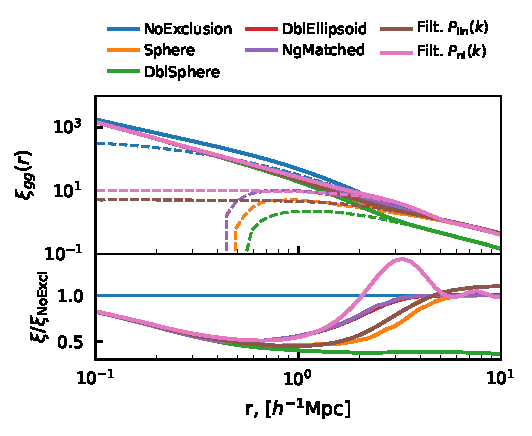
\includegraphics[width=\linewidth]{figures/halo_exclusion.pdf}
  \caption[Effect of halo exclusion]{Effects of various halo exclusion models around the transition region. Solid lines are the full $\xi_{gg}(r)$, while the dashed lines show the 2-halo term. In both cases where the halo-centre power spectrum is modified (brown and pink curves), the halo exclusion is not performed. }
  \label{fig:halo_exclusion}
\end{figure}

\section{Extending the Halo Model to Galaxies}
\label{sec:TracerHaloModel}

\subsection{HOD models}
\label{sec:theory-gal:hod}
Before we can extend the previous theory to a treatment of tracers (eg. optical galaxies), we must have a model for the expected occupation of the tracer within a given halo, $P(T|m)$, termed the halo occupation distribution (for discrete tracers such as galaxy counts, this is typically written $P(N|m)$ and must be a discrete distribution). Note that this model is assumed to depend solely on the halo mass, which perhaps surprisingly captures the majority of the behaviour of interest. There is a known second-order dependence on environment, the so-called `assembly bias' \citep{Sunayama2015}, but we do not consider it in this work.

Any HOD model is principally composed of two parts -- a parametrisation of the mean occupation of halos of a given mass, $\Nt_m$\footnote{Note that we use notation consistent with discrete tracers throughout, but these functions are generalizable to non-discrete distributions.}, and a distribution about this mean $P(N_t|\Nt_m)$ (note that throughout this work, we imply that any values $\langle N \rangle$ are functions of mass, and drop the notation from here on). The mean occupation plays the major role in providing a form for the mass dependence of typical galaxy abundances, while the distribution is crucial in calculating pair (and triplet etc.) count statistics. 

Historically, the parametrisation of the mean occupation began as a single function, but early work \citep{Kauffmann2004,Zheng2005,Zehavi2005} showed an advantage in treating `central' and `satellite' galaxies independently. In hydrodynamical simulations, these are empirically identifiable classes of galaxies, and semi-analytic methods also treat them separately. Central galaxies (in optical) tend to be large and bright, and occupy the region near the halo's central potential well. Satellite galaxies are less bright, and tend to follow the halo's density profile\footnote{This is not strictly true -- satellites may follow an alternate profile to the underlying dark matter (eg. flattening towards the center). The point is that they follow a profile. \halomod\ allows both the halo and tracer profiles to be specified independently.}.  Note that these qualitative descriptions are not necessarily true for all samples of tracers, but it typically remains useful to separate occupation of the tracer into such central and satellite classes.

Finally then, we have a mean occupation function for each class, and the total occupation is their sum:
\begin{equation}
    \Nt = \Nc + \Ns.
\end{equation}

Identifying these classes as independent is helpful in determining the distributions about the means. Halos may only contain a single central galaxy (or none at all if the sample selection does not allow it). Thus their distribution is simply Bernoulli (or Binomial with a single trial):
\begin{equation}
    N_c \sim \text{Bern}(\Nc).
\end{equation}
Satellite galaxies have been found to approximately follow Poisson distributions \citep{Kauffmann2004,Zheng2005}:
\begin{equation}
    N_s \sim \text{Pois}(\Ns).
\end{equation}

Most studies also impose what we will term the `central condition'. Explicitly, the condition states that $N_c = 0 \Rightarrow N_s = 0$ (i.e. no central galaxies in a halo implies no satellites).
It arises from the fact that central galaxies are more luminous than their satellite counterparts, and therefore for any sample selection based on luminosity (or similar) thresholds, the central galaxy will be the first to be included.  Our implementation does not enforce this condition (as there are conceivably sample selections which circumvent it), but does enable it, which simplifies some calculations.

For two-point statistics, an important quantity arising from the HOD is the mean pair counts, $\langle N_t(N_t-1) \rangle$. We wish to derive this quantity in a form explicitly dependent only on the mean occupation functions $\Nc$ and $\Ns$, for which we have specific parametrisations. We begin by noting, after \citet{Zheng2005}, that
\begin{equation}
    \langle N_t(N_t-1) \rangle = \langle N_c(N_c-1) \rangle + \langle N_s(N_s-1) \rangle + \langle N_c N_s \rangle,
\end{equation}
in which the first term on the right vanishes since $N_c$ is either $0$ or $1$, and under the assumption that $N_s$ has a Poisson distribution, we can simplify to
\begin{equation}
    \label{eq:nt_pairs}
    \langle N_t(N_t-1) \rangle = \Ns^2 + \langle N_c N_s \rangle.
\end{equation}
The last term is problematic, however if we impose the central condition, then $\langle N_c N_s \rangle = \Ns$, since we need only count halos in which $N_c = 1$. Thus, if the central condition holds, we achieve the final form
\begin{equation}
    \langle N_t(N_t-1) \rangle = \Ns(1 + \Ns).
\end{equation}

If the parameterisations for $\Nc$ and $\Ns$ do not impose the central condition then we can approximate, following \citet{Zehavi2005}, with $\langle N_c N_s \rangle = \Nc \Ns$, given that $\Ns \ll 1$ when $\Nc < 1$. For $\Nc = 0$ or 1, it is no longer an approximation, and thus for step-function parameterisations of $\Nc$, it is completely accurate (for arbitrary parameterisations of $\Ns$).

Finally, if the central condition is required, but the parameterisations of choice do not impose it (i.e. $\Ns > 0$ when $\Nc<1$, or ``satellites may exist in a particular halo where centrals do not''), one can manipulate the equations to enforce it using a common technique \citep[eg.][]{Beutler2013}, in which we set $\Ns = \Nc \Ns'$, where $\Ns'$ is the original parameterisation. In this case, the truncation of $\Nc$ forces the appropriate truncation of $\Ns$. One must be careful in this method, however,  to ensure that the HOD parameters retain the same meaning as the original. For a step-function $\Nc$ this is not a problem, but there may be subtle differences induced for smoothed truncations (these are likely to be negligible for reasonable models).

There are several parameterisations for the HOD in the literature. In this work, and correspondingly in the \verb|halomod| framework, we focus on those that utilise the separation of
central and satellite galaxies. We present a summary of those included in \textsc{halomod} in Table \ref{tab:models_hod}. 

 Most formulations contain the same essential features, so the most important features of the HOD are present in the simplest case. For the central term: a step function characterised by a step at the parameter $M_\text{min}$, which is heavily dependent on the sample selection. The deeper the survey, the lower this parameter will be. The satellite term is primarily characterised by a power law which quantifies the growth of galaxies with halo mass by the index $\alpha$, and a scaling mass $M_1$ which is the mass at which an average halo in the sample contains a single satellite galaxy.

\begin{figure}
\centering
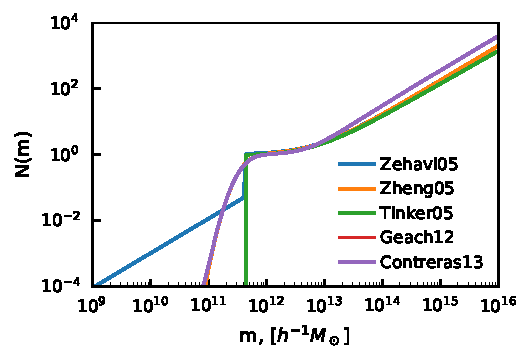
\includegraphics[width=\linewidth]{figures/hod_models.pdf} 
\caption[Halo occupation for several parameterisations]{Total halo occupation for several parameterisations, highlighting the core similarities and differences between the models. Note that the central condition is false for the models shown.}
\label{fig:hod}	
\end{figure}

The various refinements to this general structure include smoothing the truncation of central galaxies assuming a log-normal distribution of halo masses at this threshold, and truncating the satellite power law at an arbitrary mass scale $M_0$. Further refinements can be specific to a certain kind of sampling, for example samples gained at different wavelengths. An illustrative plot of the core similarities and detailed differences can be found in figure \ref{fig:hod}.



\subsection{Extension of framework to galaxies}
\label{sec:theory-gal:framework}
The extension of equations \ref{eq:dmcorr1}, \ref{eq:dmpower1} and \ref{eq:dmpower2} to include galaxies is relatively simple under the assumption that all galaxies reside in halos, and their intra-halo abundance follows that of the density profile. 

The primary modification of the DM equations is to replace factors of $m/\bar{\rho}$ with $N_t(m)/\bar{n}_g$, where $N_t(m)$ is the mean occupation function from the HOD (where for simplicity we omit angle brackets for the rest of this work), and $\bar{n}_g$ is the mean number density of galaxies,
\begin{equation}
    \label{eq:meandens}
 \bar{n}_g = \int n(m)N_t(m) dm.
\end{equation}
With this modification the 2-halo term is simply described by
\begin{equation}
    I_g(k,m) = n(m) u(k|m) N_t(m)/\bar{n}_g,
\end{equation}
which serves as a direct replacement for $I_\text{DM}$ in equations \ref{eq:dmpower2a} and \ref{eq:dmpower2}.


The 1-halo term needs a little more care. The primary modification gives
\begin{equation}
\label{eq:galcoor1}
1 + \xi_g^{1h}(r) = \frac{1}{\bar{n}_g^2}\int n(m) \frac{\langle N_t(N_t-1) \rangle}{2} \lambda(r|m) dm,
\end{equation}
however using the formalism of \S\ref{sec:theory-gal:hod}, we can separate the pair counts into contributions from central-satellite ($c-s$) pairs, and satellite-satellite ($s-s$) pairs (cf. Eq. \ref{eq:nt_pairs}). The first of these is a one-point quantity dependent only on the profile, rather than the self-convolution. Thus we have, for the correlations
\begin{equation}
1 + \xi_g^{1h}(r) = \frac{2}{\bar{n}_g^2}\int n(m) \left[\langle N_c N_s \rangle \rho(r|m) + N_s^2 \lambda(r|m)\right] dm,
\end{equation}
where the quantity $\langle N_c N_s \rangle$ is treated differently depending on whether the central condition is imposed (cf. \S\ref{sec:theory-gal:hod}). The Fourier-space counterpart is defined likewise.




\subsection{Derived Quantities}
There are several quantities of interest which can be derived from the HM/HOD framework.

Firstly, on large scales, where $u\rightarrow1$, and the 1-halo term is negligible, the 2-halo term is approximated by
\begin{equation}
 P_{gg}(k) \approx b^2_\text{eff}P_m(k),
\end{equation}
where
\begin{equation}
\label{eq:beff}
 b_\text{eff} = \frac{1}{\bar{n}_g}\int n(m)b(m)N_t(m) dm
\end{equation}
is called the ``effective bias".

We may likewise calculate an ``effective concentration" which is the mean halo concentration within the sample:
\begin{equation}
     c_\text{eff} = \frac{1}{\bar{n}_g}\int n(m)c(m)N_t(m) dm,
\end{equation}
and an ``effective mass":
\begin{equation}
     M_\text{eff} = \frac{1}{\bar{n}_g}\int n(m)mN_t(m) dm.
\end{equation}

An important quantity in studies of galaxy formation and evolution is the fraction of galaxies that are satellites. The evolution of this quantity through time can trace the effects of various physical processes. It is simply defined as
\begin{equation}
    f_\text{sat} = \frac{\int n(m) N_s(m) dm}{\int n(m) N_t(m) dm}.
\end{equation}



\section{The \textsc{halomod} library}
\label{sec:halomod}

In this section we present our new implementation of the HM, \textsc{halomod}. Our intention is first to give an overview of the philosophy behind, and general characteristics and features of the code. From there, we describe in detail various parts of the code, beginning in \S\ref{sec:halomod:frameworks} with the ``frameworks" which tie together the various components, and then the individual components themselves in \S\ref{sec:halomod:components}. These sections have a pragmatic focus, introducing any pertinent numerical techniques, and summarising the various models included. Finally, we comment on some of the extra functionality present in the package in \S\ref{sec:halomod:extra}.


 
\subsection{Philosophy and Architecture}
\label{sec:halomod:overview}
\textsc{Halomod} is a Python package, built on the \textsc{hmf} package\footnote{\url{https://github.com/steven-murray/hmf}} \citep{Murray2013a}, which contains the necessary components and algorithms to calculate HM quantities, and also tracer statistics via a HOD\footnote{For now, it only implements the two-point statistics, but this will be expanded in future versions.}. 
\textsc{hmf} provides modules for cosmology, transfer functions, spatial filters, mass definitions and mass functions, along with defining a coherent and flexible software framework. 
\halomod\ inherits that framework and provides halo profiles, concentration relations, bias functions, halo exclusion models and HOD models and combines them into the full halo model.

%\bd{I think it's a little unclear how hmf and halomod are related. What exactly does halomod take from hmf? It's more than just the mass function module, right?}

%As discussed in the introduction, HM studies are a burgeoning field, especially in the interpretation of large galaxy surveys via HOD fits to galaxy two-point statistics. Furthermore, the compartmentalisation of the technique into various components (eg. halo profile, mass function etc.) provides opportunity to enhance analyses by improving individual components. These basic factors motivate the development of a code which has the following properties: \bd{ah, that's what I was looking for in the intro!} \sgm{OK need to discuss this}


The principles outlined in the introduction, i.e.  ``Intuitive'', ``Simple'', ``Efficient'', ``Extendible/Flexible'', ``Comprehensive'' and ``Open'', have been the guiding principles in the development of \textsc{halomod} (and also \textsc{hmf}). Our code provides a well-defined architecture for defining components and frameworks for halo modelling, including many basic and derived quantities of interest, and a large fraction of the available models in the literature. Each component is completely flexible, either by supplying custom parameters or entirely new parameterisations \textit{without touching the source code}. We now expand upon some of these aspects.

Note that many of the features that we discuss in this section reflect updates to the \textsc{hmf} package (compared to its presentation in \citet{Murray2013}), which are inherited in \textsc{halomod}. Furthermore, clearly this paper represents a snapshot of the package in time, with updates likely to occur. 

\subsubsection{Intuitive Usage}
\label{sec:halomod:overview:usage}
To demonstrate the intuitive usage of \halomod, it is perhaps most useful to give a quick example of how \verb|halomod| can be invoked. 
Necessarily, the following example is both simple and rather arbitrary, but it should give a flavour of the usage of \halomod.

To create a new halo model class (this one will support galaxy power spectra and correlation functions) does not require passing any parameters, as all parameters have reasonable defaults:
%\ifthenelse{\boolean{useminted}}{%
%	\begin{minted}{python}
%	import halomod as hm
%	tr = hm.TracerHaloModel()
%	\end{minted}
%}
After creating the model, all of the relevant quantities may be accessed as attributes (in fact, they are not simple attributes that have been pre-computed, they are calculated lazily on first access and then cached).
Thus, we can plot the auto-correlation function of galaxies, for example; 
%\begin{minted}{python}
%plt.loglog(tr.r, tr.corr_auto_tracer, label='z=0')
%\end{minted}
\begin{lstlisting}[language=Python]
plt.loglog(tr.r, tr.corr_auto_tracer, label='z=0')
\end{lstlisting}
To update a parameter, one can simply set it on the instance, so for example to change the redshift and plot the new correlation function:
%\begin{minted}{python}
%
%\end{minted}
\begin{lstlisting}[language=Python]
	tr.z = 1
	plt.loglog(tr.r, tr.corr_auto_tracer, label='z=1')
\end{lstlisting}
Updating any parameter immediately invalidates the cache of quantities that depend on it, and thus that quantity is recalculated (but not quantities on which it depends that don't themselves depend on the changed parameter -- like the cosmological transfer function in this example). 

Every sub-component of the halo model (see the following sections) allows its parameters to be changed directly from this top-level interface. So, if we wanted to update the $M_{\rm min}$ parameter of the halo model, we could simply do
%\begin{minted}{python}
%
%\end{minted}
\begin{lstlisting}[language=Python]
tr.hod_params = {"M_min": 8.0}
plt.loglog(tr.r, tr.corr_auto_tracer, label='Mmin=8')
\end{lstlisting}
After applying relevant axis labels, we then produce Fig. \ref{fig:toy_example}.

\begin{figure}
    \centering
    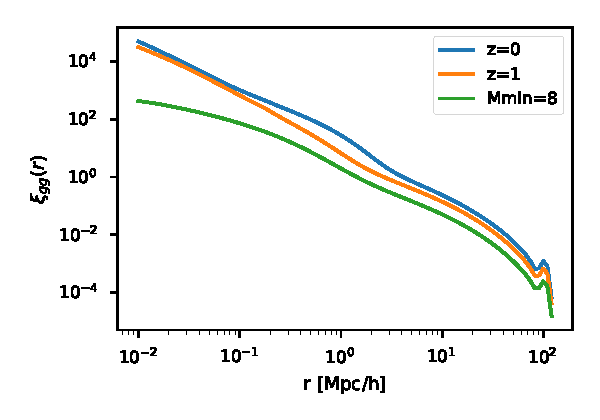
\includegraphics[width=\linewidth,trim={0 0.2cm 0 0},clip=true]{figures/toy_example.pdf}
    \caption{Simple example of galaxy auto-correlation functions produced with three inputs (two different redshifts and a different HOD model).
    Notice the BAO peak at $\sim100 h^{-1}{\rm Mpc}$. Code to produce the figure is presented in \S\ref{sec:halomod:overview:usage}.}
    \label{fig:toy_example}
\end{figure}

\subsubsection{Simple Conceptual Framework}
\label{sec:halomod:overview:concept}
The backbone of \textsc{halomod}, directly inherited from \textsc{hmf}, is split into two categories: `frameworks' and `components', which are well-defined by a base class, \framework\ and \component\ respectively. Individual elements of the calculation, such as a halo profile, HMF fitting function, or any other unit which may be calculated in more than one way (e.g., growth factors) are represented by a \component. \texttt{Framework}s are the structures which tie each \component\ together to calculate a set of quantities (e.g., correlation functions, power spectra or mass functions). Frameworks may also contain other frameworks (for example the \texttt{Cross\-Correlation} framework contains two \texttt{TracerHaloModel} frameworks -- one for each tracer to be cross-correlated).

This structure makes it simple to identify a component of interest for extended modelling, and provides a common interface and set of methods to each type. For example, if one is developing a new improved model of halo bias, it is clearly identified as a \component, with a particular structure. Its place in the overall framework is well-specified, it by default receives any defining parameters it requires, and specific examples of implementations of other models of the component are easily found in the \verb|bias| module. 

It is expected that the most common usage will be to create a \framework\ instance, and access available quantities through it. Our general approach has been to treat frameworks as a self-contained unit. This means that all parameters are passed to the initial constructor, after which every relevant quantity is ready for immediate access, without method-specific parameters. Indeed, to the user, once a \framework\ instance has been created (with all its options), any derived quantity (such as mass functions, correlation functions, mass variance etc.) is accessed just like a stored variable. 

This approach is not typical of much software -- usually there is benefit in segregating object-wide variables from method-specific ones. However, we find in our case that most variables are used across many methods, and are more naturally interpreted as being a part of the framework itself. 

In fact, our adherence to this approach is bolstered by our generic distinction (within \texttt{Framework}s) between a \parameter\ and a \cached. Every input variable is treated as a class-wide \parameter, which receives its own characteristics (this is very useful for our caching mechanism, see \S\ref{sec:halomod:overview:efficiency}). Every evaluated quantity is treated as a \cached, which likewise has its own properties. The set of all \texttt{parameter}s of a given \framework\ is then a unique description of the entire object (and can be used to test equality between framework instances). 

Though the state of a \framework\ is defined by its parameters, we provide a simple mechanism of modifying the parameters for dynamic calculations, through an \verb|update| method, which can receive any \parameter\ (or, as noted in the previous subsection, simply by setting the attribute)\footnote{This method is defined in the base \texttt{Framework} class, and is therefore simply inherited by any specific framework.}.

Our approach to the passing of parameters has been to provide defaults for \textit{every} variable in a \framework\footnote{These defaults are currently majoritarily static, but we plan on dynamifying them in future versions.}. These defaults are chosen to be broadly in line with the most common usage, which greatly simplifies common tasks. However, it must be noted that this has the drawback that if user code relies on defaults, and code updates modify them, then results can vary without being noticed. 

In summary, the architecture of \hmf\ and \halomod\ consists of
\begin{itemize}
    \item A flexible \component\ for each independent element of the HM.
    \item A range of specific \textit{models} for each \component.
    \item Powerful \framework\ classes that synthesise multiple \verb|Components| to provide plug-and-play functionality.
    \item \texttt{Frameworks} consist of \texttt{parameters} which can be input and modified by the user, and \cached\ objects, which are calculated from the \verb|parameters| and are read-only and always consistent with the current settings.
\end{itemize}



\subsubsection{Efficiency}
\label{sec:halomod:overview:efficiency}

While \halomod\ generally prioritizes ease-of-use over efficiency, it is optimized in a number of ways:
\begin{itemize}
    \item Heavy use of \textsc{numpy}\footnote{\url{http://www.numpy.org/}} to enable vectorized calculations, close to compiled code performance in most cases.
    \item Calculation of all quantities at a fixed set of user-defined vectors (as opposed to providing methods that ingest evaluated variables such as mass or wavenumber)\footnote{An exception to this rule applies in the case of the 2-halo term, which can require two sequential Hankel transforms. For this, we evaluate $\xi_{2h}(r)$ on a background grid of $r$ which adequately captures the behaviour required for the inverse transform, and we interpolate this grid for the user's input vector of $r$.}.
    \item Use of ``just-in-time'' (JIT) compiled functions (via \textsc{numba}\footnote{\url{http://numba.pydata.org/}}) where vectorization is impossible or disadvantageous.
    \item A novel and robust caching system with extremely accurate and efficient cache invalidation (i.e. cached quantities always stay up-to-date with parameter changes, but nothing updates that doesn't have to). See \ref{app:caching} for details on this system, which utilises the core architecture of the \framework\ to achieve its goals.
\end{itemize}

%We make heavy use of the excellent \textsc{numpy}\footnote{\url{http://www.numpy.org/}} package to enable optimized compiled code performance in the background for many of the array calculations. With careful use of broadcasting and vectorization, the bulk of the calculations are close to as efficient as one would expect from compiled code, within the simplicity and readability of the interpreted language.

%In concert with this, we choose to implement all methods discretely at a set of pre-defined vectors. That is, instead of providing, say, a mass function method which takes mass an input, the mass function is defined on the instance only
%at the masses input to the class itself. Thus all other quantities depending
%on the mass function expect only to receive a mass function defined at those
%same masses. This allows significant vectorization, but also some extra simplicity of the API -- the user sets the evaluated variables (such as mass or wavenumber) once at initialization, and all quantities are kept fixed and consistent thereafter. 

%A slight exception to this rule applies to halo model correlation functions and power spectra (i.e. not the linear power spectra). In this case, since we sometimes need to convert one to the other (via Hankel transform), \verb|halomod| specifies a backend table of co-ordinates $r_i$ and $k_i$ which are defined to cover the range and have the appropriate resolution to enable the Hankel transform to be accurate. The quantities evaluated on these tables are then interpolated robustly to a user-specified set of co-ordinates.

%In cases of computational bottlenecks where vectorization is not an option due to memory consumption, we have implemented optional ``just-in-time" (JIT) compiled functions using the \textsc{numba} package\footnote{\url{http://numba.pydata.org/}}. Though these functions reduce code readability and extendibility to some extent, they can improve speeds in small bottleneck routines to almost-compiled-code standards. Furthermore, we always implement a pure-python basic function for testing, and the JIT-compiled function is only called in its place if the user has \textsc{numba} installed. 

%We make various other functional-level performance improvements which we will refer to in their own context. However, possibly the most useful performance enhancement is \textsc{halomod}'s caching system.


\subsubsection{Flexibility}
\label{sec:halomod:overview:flexibility}
We have referred to our imposed dichotomy between \framework\ and \component\ objects, and in the previous subsection we outlined a performance benefit derived from the internal structure of the \framework. Likewise, we have implemented a uniform convention for \component\ specification which enhances flexibility.

Any component that is implemented as a \component\ is a variable within a \framework. As such, it is determined by passing a \parameter, in the form of either a string representing the name of the model, or the class itself. 
%In order to avoid updating endless lists of available models to be selected by the string identifier, we implement a basic \verb|get_model| function which locates and returns appropriate models based on our conventions. 

Every \component\ has a top-level dictionary specifying the model-specific parameters and their default values (these are not fundamental quantities used in the calculation, eg. $\nu$ in the $f(\nu)$ for the HMF, but rather free parameters of the model, if any). These are processed by the base class so that any newly defined model automatically has them available. In the \framework, the model parameters are passed, by convention, as \verb|<cmpnt>_params|. Furthermore, the \verb|update| method in each \framework\ intelligently updates parameter dictionaries so that previous updates are persistent unless explicitly overwritten.

This general system offers the highest level of flexibility and extendibility. In a single session, it is extremely simple to switch between several models for a given component, thereby making useful comparisons (and this without needing to recalculate basic quantities that do not depend on the variable component). On the other hand, using entirely new custom models can be achieved without modifying the source code, by inheriting from the base \component\ and passing the new model directly to a \framework. We reiterate this point, as we expect this to be particularly advantageous in the current climate of rapid development: \texttt{Components} are \textit{pluggable}. A user can write their own new HMF fit, or bias function, or HOD model, in their own notebook (or wherever they write code), and use it right away in the context of the full halo model. 

Furthermore, to a greater or lesser degree, each \component\ has built-in methods which either remove the burden on the user, or supply extra functionality for free when the user develops a new model. This is perhaps most clear in the \verb|Profiles| component (cf. \S\ref{sec:halomod:components:profile}), though some components have very little to add to the basic model (eg. the \verb|Bias| component, cf. \S\ref{sec:halomod:components:bias}). 

\texttt{Components} are primarily designed to integrate with the \texttt{Frameworks}, however, they are not limited to this usage. They are also intended to be useful in their own right, for more specific applications. 

%Summarily, the \component\ architecture of \textsc{halomod} is geared to provide flexibility and extendibility for crucial developments in the field in the years to come.

\subsubsection{Interoperability}
\textsc{halomod} is intended to be a package that is adopted and maintained by the community. To this end, it uses well-known and well-maintained libraries to enable much of its functionality. 
For example, cosmologies are defined via \textsc{astropy}\footnote{\url{https://www.astropy.org/}} and we use the standard open-source \textsc{numpy} and \textsc{scipy} packages for numeric and scientific routines. 
We also adopt the open-source \textsc{hankel}\footnote{\url{https://github.com/steven-murray/hankel}} \citep{Murray2019} package for computing some of the Hankel transforms.

We also provide extensive interoperability with the \textsc{Colossus} code\footnote{\url{http://www.benediktdiemer.com/code/colossus/}} \citep{Diemer2018}, by providing component constructors for models contained in \textsc{Colossus}. 
In practice, this means that the user can invoke something like the following
%\begin{minted}{python}
%
%\end{minted}
\begin{lstlisting}[language=Python]
	bias = make_colossus_bias("comparat17")
	model = TracerHaloModel(bias_model=bias)
\end{lstlisting}
and get the full range of functionality from the \textsc{Colossus}-defined bias model within the \textsc{halomod} framework (even setting of model-dependent parameters).
At the time of publishing, these constructors are defined for bias and halo concentration models, as these models are part of the core functionality of \textsc{Colossus} and thus there is a real chance that the models may exist in \textsc{Colossus} and not \textsc{halomod}. 

Furthermore, versions of \textsc{colossus} from v1.2.16 onwards have implemented a simple pair of functions enabling conversion of \textsc{astropy} cosmologies to and from the native \textsc{colossus} cosmologies. 
Since \halomod\ cosmologies are essentially derived from \textsc{astropy}, this enables a greater degree of interoperability between \textsc{colossus}
 and \halomod.
 
\subsection{Frameworks}
\label{sec:halomod:frameworks}
In this section we present two of the frameworks that \textsc{halomod} provides. We note that several other frameworks are found in the \textsc{hmf} package, from which those presented here inherit. Furthermore, \textsc{halomod} also provides a \verb|DMHaloModel| framework for calculating non-linear matter power spectra and correlation functions, and a \texttt{Cross\-Correlations} framework for cross-correlating two tracers. We do not present these here explicitly, but note that the \verb|DMHaloModel| is a strict subset of the \verb|TracerHaloModel| which we do present.

\subsubsection{Base Halo Model}
\label{sec:halomod:frameworks:base}
The basic framework in \textsc{halomod} is \verb|TracerHaloModel|, which provides general access to most derived quantities relating to two-point statistics. Table \ref{tab:halomodel_parameters} contains a useful summary of parameters for \verb|TracerHaloModel|, giving an indication of its flexibility. Likewise, table \ref{tab:halomodel_properties} lists the available properties. We note that these are expected to be updated and expanded in future versions, and thus are not intended to provide a strict API, but rather an illustrative summary.


%%%%%%%%%%%%%%%%%%%%%%%%%%%%%%%%%%%%%%%%%%%%%%%%%%%%%%%%%%
% HaloModel parameter table
%%%%%%%%%%%%%%%%%%%%%%%%%%%%%%%%%%%%%%%%%%%%%%%%%%%%%%%%%%
\begin{table*}
\centering
 {\tabulinesep=1mm
\begin{tabu} to \linewidth{X[1.6l]X[1.4l]X[5l]} 
\toprule[0.05cm]
\textsc{Parameter} & \textsc{Default}$^\dagger$ & \textsc{Description} \\
\toprule[0.05cm]

\multicolumn{2}{l}{\textsc{Components/Parameters}*} \\
\texttt{cosmo\_<>} & \texttt{Planck13} & Underlying cosmology. Must be an \texttt{FLRW} object from \textsc{astropy}. This model differs from other \texttt{Components}, being passed as an \textit{instance}, not a \textit{class}.\\
\texttt{transfer\_<>} & \texttt{CAMB} & A model to use for the transfer function. \\
\texttt{growth\_<>} & \texttt{GrowthFactor} & A model for the growth function. The default is to perform the explicit integration.\\
\texttt{mdef\_<>} & \texttt{None} & A mass definition (default is the definition under which the chosen \texttt{hmf} was measured). \\
\texttt{hmf\_<>} & \texttt{Tinker08} & A model specifying the HMF fitting function, $\nu f(\nu)$.\\
\texttt{filter\_<>}& \texttt{TopHat} & A filter function model. \\   
\texttt{hod\_<>} & \texttt{Zehavi05} & A HOD model. \\   
 \texttt{profile\_<>} & \texttt{NFW} & A halo profile. \\
 \texttt{concentration\_<>}  & \texttt{Duffy08} & A concentration-mass-redshift relation \\
 \texttt{bias\_<>} & \texttt{Tinker10} & A scale-independent linear bias model. \\
 \texttt{sd\_bias\_<>}& \texttt{Tinker\_SD05} & A model for the scale-dependence of the linear bias. \\
  \texttt{exclusion\_<>} & \texttt{NgMatched} & A halo exclusion model. \\
 
  
\midrule
\multicolumn{2}{l}{\textsc{Resolution/Location}} \\
\texttt{lnk\_min}, \texttt{lnk\_max}, \texttt{dlnk} & -8,8, 0.05  & Min/Max/$\Delta$ logarithmic wavenumber for linear power spectra and tabulated halo model spectra\\
\texttt{hm\_logk\_min}, \texttt{hm\_logk\_max}, \texttt{hm\_dlogk} & -2.5,1.5, 0.05  & Min/Max/$\Delta$ logarithmic wavenumber for output halo model spectra \\
\texttt{dlog10m} & 0.01 & Logarithmic mass interval \\
\texttt{rmin}, \texttt{rmax}, \texttt{rnum}, \texttt{rlog} & 0.1, 50.0, 20, True & Min/Max/\# for pair-separation vector, and whether its vector should be equi-log-spaced. \\
\texttt{r\_table\_num} & 100 & Length of background table of $r$ \\

\midrule
\multicolumn{2}{l}{\textsc{Physical}} \\
\texttt{sigma\_8} & 0.8344 & Normalisation of power spectrum, $\sigma_8$ \\
\texttt{n} & 0.9624 & Spectral index, $n_s$ \\
\texttt{z} & 0.0 & Redshift \\
\texttt{delta\_c} & 1.686 & Critical overdensity for collapse, $\delta_c$. \\
\texttt{ng} & None & Optional specification of mean galaxy density. If present, an HOD parameter (generally $M_\text{min}$) is fixed. \\

\midrule
\multicolumn{2}{l}{\textsc{Options}} \\
\texttt{takahashi} & True & Apply updated \textsc{halofit} coefficients from \citet{Takahashi2012}  \\
\texttt{hc\_spectrum} & Nonlinear & Model for $P_{hh}^c(k)$. Either ``linear", ``nonlinear" (\textsc{halofit}), or ``filtered-nl" (smoothed on a scale of 2$h^{-1}$Mpc). \\
\texttt{force\_1halo\_turnover} & True & Whether to cut off the 1-halo power on extremely large scales.  \\

\bottomrule[0.05cm]
\end{tabu}}
\caption[Summary of parameters included in \texttt{TracerHaloModel}]{All parameters of \texttt{TracerHaloModel}. Parameters in the ``Components/Parameters" section are each specified by two parameters, ending in \texttt{model} and \texttt{params} (i.e. \texttt{hmf\_<>} represents two parameters: \texttt{hmf\_model} and \texttt{hmf\_params}). Using the HMF as an example, \texttt{hmf\_model} is the actual model specification, and this is listed in the \textsc{Default} column. Conversely, \texttt{hmf\_params} is a dictionary of parameters for the model, which is not listed in this table, but can be found in the online API documentation. The parameters available for each \textit{model} within a particular component may be different. Notice also that the physical parameters $\sigma_8$ and $n_s$ are directly set within the framework, rather than being a part of the cosmology parameters. The reason for this is outlined in \S\ref{sec:halomod:components:cosmology}.}
\label{tab:halomodel_parameters}
\end{table*}

%%%%%%%%%%%%%%%%%%%%%%%%%%%%%%%%%%%%%%%%%%%%%%%%%%%%%%%%%%
% HaloModel properties table
%%%%%%%%%%%%%%%%%%%%%%%%%%%%%%%%%%%%%%%%%%%%%%%%%%%%%%%%%%
\begin{table*}
\centering
 {\tabulinesep=1mm
\begin{tabu} to \linewidth{X[1l]X[4.5l]} 
\toprule[0.05cm]
\textsc{Type} & \textsc{Quantities}*  \\
\toprule[0.05cm]
Scalar & $b_\text{eff}$, $f_\text{cen}$, $f_\text{sat}$, $D^+(z)$, $M_\text{eff}$, $M_\star$, $\bar{\rho}(z)$, $\bar{n}_g$, $n_\text{eff}$ \\
Length-$m$ & $R$, $b$, $\bar{c}$, $\nu f(\nu)$, $\frac{dn}{d\ln m}$, $\frac{dn}{d\log_{10} m}$, $\frac{dn}{d m}$, $n(>m)$, $\Nc$, $\Ns$, $\Nt$, $L(n=1)$, $\ln \sigma^{-1}$, $\nu$,  $\rho(>m)$, $\rho(<m)$ \\
Length-$k$ & $T$, $P_m$, $P_{m, \text{halofit}}$, $\Delta^2$, $\Delta^2_\text{halofit}$, $P_{gg}^{ss}$, $P_{gg}^{2h}$, $P_{mm}$, $P_{mm}^{1h}$, $P_{mm}^{2h}$, $P_{mg}^{1h}$, $P_{mg}^{2h}$, $P_{mg}$ \\
Length-$r$ & $\xi_{gg}^{1h}$, $\xi_{gg}^{cs}$, $\xi_{gg}^{ss}$, $\xi_{gg}^{2h}$, $\xi_{gg}$, $\xi_{DM}^{1h}$, $\xi_{DM}^{2h}$, $\xi_{DM}$, $\xi_m$, $\xi_{m, \text{halofit}}$, $\xi_{mg}^{1h}$, $\xi_{mg}^{2h}$, $\xi_{mg}$, $S(\xi_m(r))$ \\
Function of $r,m$ & $\rho$, $\lambda$ \\
Function of $k,m$ & $u$ \\
%Function of $k,r$ & $W(kr)$ \\
 
\bottomrule[0.05cm]
\end{tabu}}
\caption[All included properties of \texttt{TracerHaloModel}]{All properties of \texttt{TracerHaloModel}. Listed are those quantities that are directly accessible as explicit properties. Other quantities, such as the window function, are accessible indirectly through a model instance variable.}
\label{tab:halomodel_properties}
\end{table*}


Some of the features of the \verb|HaloModel| framework, ignoring contributions of individual components, are as follows.

\paragraph*{Mean density matching} 
Most HOD parameterisations have a parameter $M_\text{min}$, which either explicitly or loosely defines the minimum halo mass expected to host galaxies in the sample. This parameter is tightly correlated with the mean galaxy density, as it determines the lower limit of the integral in Eq. \ref{eq:meandens}. It is common (though not ubiquitous) in survey analyses to let the known value of $\bar{n}_g$ determine $M_\text{min}$ (given other parameters of the HOD) \citep[eg][]{Beutler2013}. \verb|TracerHaloModel| supports this technique for all HOD models, either by direct cumulative integration, or by numerical minimization. This is caught at every update of parameters.

\paragraph*{Mass range setting}
The mass range in \verb|TracerHaloModel| is user-definable, but sets intelligent limits. An upper limit of $M_\text{max} = 10^{18}h^{-1}M_\odot$ is set to ensure convergence of mass integral, and the lower limit is set to $M_\text{min} = 10^{0}h^{-1}M_\odot$ for matter calculations, and is based on the value of $M_\text{min}$ in the HOD for tracer calculations. For step-function models, the lower limit is exactly $M_\text{min}$, which increases accuracy in an important regime. For smooth-cutoff models, the lower limit is determined by the \verb|mmin| property of the HOD (see \S\ref{sec:halomod:components:hod}).

\paragraph*{Halo-centre power spectrum}
A key quantity in the large-scale clustering is the power spectrum of halo centres, $P_{hh}^c(k)$ (cf. \S\ref{sec:theory:2halo} and \S\ref{sec:theory:exclusion}). This can be modelled via the linear matter power, nonlinear matter power, or even some smoothed version of either. We leave this choice free for the user, through the parameter \verb|hc_spectrum|. 

\paragraph*{Convolutions}
The satellite-satellite term can be calculated directly in real-space if and only if there is an analytic solution for the self-convolution of the halo profile. \verb|TracerHaloModel| uses this form directly if possible, saving integration time, but resorts to a calculation in Fourier-space (and subsequent Hankel transform) if necessary. 

\paragraph*{Hankel transforms} 
The Hankel transform is a delicate operation, involving the integration of a highly oscillatory function. We use a novel method for performing this transform, which we detail in \ref{app:hankel}.

\paragraph*{Tabulation}
The Hankel transform of a power spectrum to a correlation function is typically relatively simple and accurate(using the framework for Hankel transforms defined in \ref{app:hankel}).
This is especially so since the power spectrum is naturally defined over a large range and at quite high resolution (as is required for the calculation of the mass variance, for example). 
However, the converse is not true -- transforming a correlation function to a power spectrum is typically quite limited in its range of accuracy. 

It is thus tempting to calculate power spectra at the $k$-vector at which the linear power spectrum is defined, and consider only ever transforming into real space. If this is the case, the vector of $r$ at which the correlation functions are defined can be low-resolution and limited in range, since it would be used only as an output, not as an input to some other function that requires it to be high-resolution.

However, this turns out not to be realistic in practice. 
In particular, some models of halo exclusion mix a scale $r$ -- related to the halo radius -- with the 2-halo power spectrum. Scale-dependent bias does likewise. To obtain a standard $P(k)$ thus requires performing a Hankel transform of the power \textit{at each} $r$, then an inverse Hankel transform to get back to $P(k)$. 

This requires using a higher-resolution, and importantly, large-range vector of $r$ for the intermediate correlation function. Furthermore, the calculation must be confident that the vector of $r$ is suitably well-chosen. We thus use a set tabulated background $r$ vector, and interpolate the results of $\xi(r)$ onto the user-provided $r$-vector. 

We also provide an option for the user to define a more limited range of $k$ at which to output the halo model power spectra, and these are also interpolated from their base table, which is defined on the $k$-vector used for the linear spectra. 

Problematically, the Hankel transform algorithm we employ often requires \textit{extrapolated} values of the integrand in order for the integral to converge for some scales\footnote{This is partly because the default $k$ range is quite small, as seen in Table \ref{tab:halomodel_parameters}. However, for numerical transfer functions such as those from CAMB, the intrinsically calculated range of $k$ is rather small and requires extrapolation even onto the set of $k$ input by the user.}, particularly when transforming from $\xi(r)$ to $P(k)$.
Typical cubic spline interpolation performs very poorly on extrapolation in general, often blowing up so much that the transform can be completely ruined.
We implement a robust \verb|ExtendedSpline| object to circumvent these issues. 
The \verb|ExtendedSpline| interpolates (typically with cubic interpolation) interior to the given co-ordinates, but is supplemented by settable conditions at both ends. 
The conditions at either end can be to return zeros, to continue to extrapolate the spline, to return some user-defined asymptotic function (which is normalised to match at the boundary point) or to extrapolate linearly in log-space (i.e. assuming the asymptotic behaviour on either end of the function is roughly power-law-like). 
We typically set correlation functions to return zero above the point at which they cross zero (typically about 125 Mpc/$h$) and exhibit power-law behaviour on small scales (as long as the slope of the function is shallower than an index of -2 the smallest scales do not contribute significantly in any case). 
Power spectra are considered to be power-laws at high $k$ and power laws explicitly with an index of $n_s$ at low $k$ (except when they are cut-off for some reason, like the 1-halo term, in which case they return zero below the cutoff).

We provide callable functions for each of the power spectra and correlation functions of the halo model, based on these extended splines evaluated on the high-resolution background tabulated data. 
Nevertheless, we still provide the default evaluation of these splines on the user-defined $r$ and $k$ vectors. 


\paragraph*{1-halo turnover}
At large scales, the 1-halo power spectrum converges to a non-zero constant (this is clear from Eq. \ref{eq:dmpower1}, since $u$ asymptotes to unity as $k\rightarrow0$). This is generally considered to be the ``shot-noise'' term, and is clearly unphysical when considering a smooth distribution. 
\verb|TracerHaloModel| offers to force the 1-halo term to turnover on scales larger than about 10 halo radii. 

Explicitly, it changes the lower mass limit of the integration in Eq. \ref{eq:dmpower1} to be
\begin{equation}
    m_{\rm lim}(k) = \frac{4\pi}{3} \left(\frac{\pi}{10k}\right)^3 \bar{\rho}_0 \Delta_h.
\end{equation}

\subsubsection{Projected correlation function}
\label{sec:projcorr}
In analyses of galaxy surveys, it is more common to measure \textit{projected}, rather than real-space, correlation functions (another alternative is the \textit{angular} CF, which we outline in the next section).
We provide an extended framework, inheriting from \verb|TracerHaloModel|, for this calculation. The primary reason it is separated from the basic class is that it requires extra parameters specific to its calculation. 
%A summary of the extra parameters and properties in the \verb|ProjectedCF| class is given in table \ref{tab:projectedCF}\ztc{This table seems to have been deprecated}. 

%%%%%%%%%%%%%%%%%%%%%%%%%%%%%%%%%%%%%%%%%%%%%%%%%%%%%%%%%%
% ProjectedCF properties table
%%%%%%%%%%%%%%%%%%%%%%%%%%%%%%%%%%%%%%%%%%%%%%%%%%%%%%%%%%
% \begin{table*}
% \centering
%  {\tabulinesep=1mm
% \begin{tabu} to \linewidth{X[2l]X[4.5l]} 
% \toprule[0.05cm]
% \multicolumn{2}{l}{\textsc{Parameters}} \\
% \texttt{rp\_min}, \texttt{rp\_max}, \texttt{rp\_num} & Min/Max/Length of projected scale vector \\  
% \texttt{rp\_log} & Whether to use log-scales for the projected scale vector\\
% \texttt{proj\_limit} & Optional upper limit on integral (Eq. \ref{eq:wprp}) \\
% \midrule

% \multicolumn{2}{l}{\textsc{Removed Parameters}} \\
% \texttt{r\_min} & Automatically set to \texttt{rp\_min} \\
% \texttt{r\_max} & Automatically set to \texttt{rlim} \\
% \midrule

% \multicolumn{2}{l}{\textsc{Properties}} \\
% Scalar & $r_\text{lim} \equiv \text{max}(80.0, 5r_{p,\text{max}})$, or alternatively set with \texttt{proj\_limit} \\
% Length-$r_p$ & $w_p$ \\

% \bottomrule[0.05cm]
% \end{tabu}}
% \caption[Extra parameters and properties introduced in \texttt{ProjectedCF}]{Extra parameters and properties introduced in \texttt{ProjectedCF}, as compared to \texttt{HaloModel}. Some parameters are also automatically overwritten.}
% \label{tab:projectedCF}
% \end{table*}
%%%%%%%%%%%%%%%%%%%%%%%%%%%%%%%%%%%%%%%%%%%%%%%%%%%%%%%%%%


The primary addition with respect to the base \texttt{Tracer\-Halo\-Model} class is the conversion of the real-space 2PCF to projected space. The transformation from real-space to projected is defined as
\begin{equation}
	\label{eq:wprp}
	w_p(r_p) = 2\int_{r_p}^\infty \frac{r\xi(r)}{\sqrt{r^2-r_p^2}}dr.
\end{equation}
The implementation of this integral is rather delicate due to the singularity at the lower bound. 
This renders both limits of the integration non-physical, and convergence requirements must be met by both. We discuss our prescription for these limits in appendix \ref{app:proj}.

\subsubsection{Angular correlation functions}
\label{sec:halomod:frameworks:angular}
The angular correlation function between two density fields (potentially the same field in an auto-correlation) is defined as \citep{Simon2007}
\begin{equation}
    w(\theta) \approx \int_0^\infty dr_1\int_0^\infty dr_2\ p_1(r_1) p_2(r_2) \xi(R,\bar{r}),
\end{equation} 
where $p_1$ and $p_2$ are probability distributions of finding tracers from population 1 and 2 respectively at line-of-sight comoving distance $r$ (i.e. the redshift distribution of sources), and
\begin{equation}
   R \equiv \sqrt{r_1^2 + r_2^2 - 2r_1r_2 \cos \theta}, 
\end{equation}
is a projected separation, and 
\begin{equation}
   \bar{r} = (r_1+r_2)/2. 
\end{equation}

In \halomod, we exclusively use the Limber approximation \citep{Limber1953},
which is a good approximation if $p(r)$ is a wide distribution, and $\theta$ is relatively small. In this approximation we have
\begin{equation}
   w(\theta) = 2\int_0^\infty d\bar{r} p_1(\bar{r}) p_2(\bar{r}) \int_0^{\infty} d\Delta r \xi(R,\bar{r}), 
\end{equation}
where 
\begin{equation}
   R \equiv \sqrt{\bar{r}^2 \theta^2 + \Delta r^2}.
\end{equation}


\subsubsection{Warm dark matter models}
\label{sec:halomod:frameworks:wdm}
For each of the frameworks, we also implement a version suited for warm dark matter (WDM) models. The WDM frameworks are designed to set relevant default models and perform any framework-level WDM-specific modifications.

In particular, we implement the WDM transfer function from \cite{Viel2005}, the WDM-compatible concentration relation of \cite{Ludlow2016}, along with the Sharp-$k$ filter proposed by \cite{Schneider2012} and the general large-scale structure framework for WDM outlined in \cite{Smith2011a}.

\subsection{Components}
\label{sec:halomod:components}
This section provides a brief summary of each of the components within \textsc{halomod}. 
%For each, we provide a summary table, which specifies the variables and quantities available within the model, any necessary definitions, and any extra quantities provided for free. In these tables (eg. Table \ref{tab:component_transfer})\ztc{This table seems to have been deprecated}, ``Available'' refers to the quantities available within the model (i.e. those passed in to the instance), ``Required'' refers to methods that must be defined on a valid model (if one would like to make a new model), and ``Extra'' refers to other methods that are available for free on any defined model subclass. 
For each component, we provide a table or otherwise concise summary of the models already implemented within \textsc{halomod}, and a comparison plot if relevant. 


\subsubsection{Cosmology}
\label{sec:halomod:components:cosmology}
Instead of defining our own basic cosmology models, we use the mature \textsc{astropy} package\footnote{\url{http://www.astropy.org}} \citep{Robitaille2013}. In brief, this package implements a connected series of cosmogaphic models based on the Friedmann-Lemaitre-Robertson-Walker (FLRW) metric, with several standard instances based on results from CMB missions. 

We do not present the summary details here, but note that basic cosmographic quantities such as comoving distance, and density parameters such as the mean density as a function of redshift, are implemented in these models. 

One commonly misunderstood aspect of the cosmology component is that it \textit{does not} include the large-scale-structure (LSS) parameters $\sigma_8$ and the spectral index $n_s$. This is perhaps counter-intuitive, since CMB constraints such as those from WMAP and Planck typically provide constraints on these parameters as part of the fundamental cosmology, and furthermore these parameters are covariant with cosmographic parameters (especially $\sigma_8$ and $\Omega_m$). However, \textsc{astropy} cosmologies are purely cosmographic, and \hmf\ inherits this behaviour. These LSS parameters are instead provided as inputs to the \texttt{Transfer} framework for which they are necessary to determine the normalisation and slope of the power spectrum.

\subsubsection{Transfer functions}
\label{sec:halomod:components:transfer}
We provide a common interface for calculating transfer functions using a variety of methods: from analytic fits, to Boltzmann code, to importing data from file. In each case, the required function returns the logarithmic transfer as a function of logarithmic wavenumber, as lower-order splines can be accurately fit in log space. 

We use the \textsc{pycamb}\footnote{\url{https://github.com/cmbant/CAMB}} wrapper to provide on-the-fly access to \textsc{camb} routines. We also note that we include a standalone version of \textsc{halofit} that may be used to apply nonlinear corrections to any of the included power spectra.

The various transfer models included in \textsc{hmf} are summarized in Table \ref{tab:models_transfer}. A comparison of the models with default parameters is shown in figure \ref{fig:power}.

% \begin{figure}
%   \centering
%   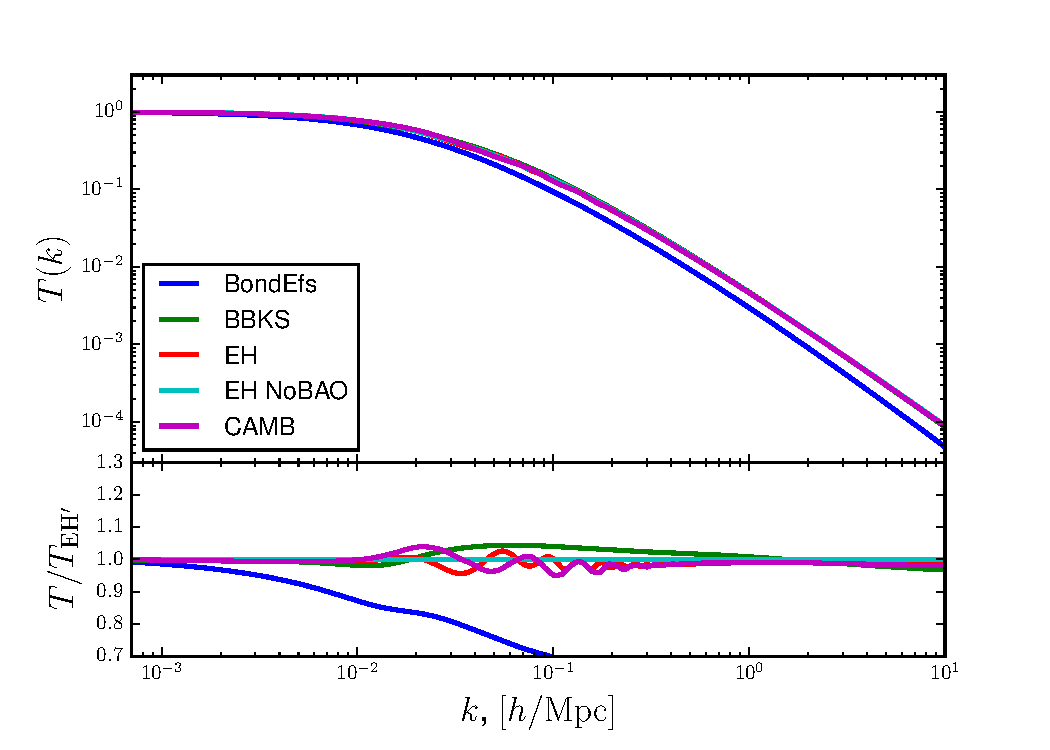
\includegraphics[width=\linewidth]{figures/transfer_fits.pdf}
%   \caption[Comparison of transfer function models, normalised at large scales]{All transfer function models in \textsc{halomod}. In each case, the transfer function is normalised to unity at very large scales. The general shape is reproduced in each case, with details of the BAO differing. The oldest fit, of \protect\citet{Bond1984}, fails to reproduce the break scale, though this is likely due to being fit to a differing cosmology. \bd{Why is this figure necessary? Doesn't it show the same as Figure 1?} }
%   \label{fig:transfer}
% \end{figure}


%%%%%%%%%%%%%%%%%%%%%%%%%%%%%%%%%%%%%%%%%%%%%%%%%%%%%%%%%%%%%%%
% \begin{table*}
% \centering
%  {\tabulinesep=1.3mm
% \begin{tabu}{X[1l]X[1l]X[4l]} 
% \toprule[0.05cm]
% \textbf{Available} &  \texttt{cosmo} & A full instance of the \textsc{astropy} FLRW class. \\

% \textbf{Required} & \texttt{lnt(lnk)} & A function returning the natural log of the unnormalised transfer function, given the natural log of the wavenumber \\

% \textbf{Extra} & None & \\
% \bottomrule[0.05cm]
% \end{tabu}}
% \caption{API summary of the \texttt{Transfer} component. \bd{this table could just be said in the text, it doesn't make immediate sense to me...}}
% \label{tab:component_transfer}
% \end{table*}
%%%%%%%%%%%%%%%%%%%%%%%%%%%%%%%%%%%%%%%%%%%%%%%%%%%%%%%%%%%%%%%


%%%%%%%%%%%%%%%%%%%%%%%%%%%%%%%%%%%%%%%%%%%%%%%%%%%%%%%%%%%%%%%
\begin{table*}
\centering
 {\tabulinesep=1.3mm
\begin{tabu}{X[1.5l]X[1l]X[3l]X[3l]} 
\toprule[0.05cm]
\textsc{Ref} & \textsc{Name} & \textsc{Formula} & \textsc{Params} \\
\midrule[0.05cm]
\citet{Bond1984} & \texttt{BondEfs} & $\left[1 + \left(\sum_{i=2}^4 (ck)^i \right)^\nu\right]^{-1/\nu}$ & $\displaystyle \frac{\Omega_m h^2}{0.3\times 0.7^2} c = (37.1,21.1,10.8)$, $\nu=1.12$ \\
\citet{Bardeen1986} & \texttt{BBKS} & $\displaystyle \frac{\ln(1+aq)}{aq} \left[\sum_{i=0}^4 (c_i q)^i\right]^{-1/4}$ & $\displaystyle q=\frac{k\exp(\Omega_b(1 + \sqrt{2h}/\Omega_m))}{\Gamma}$, $\Gamma = \Omega_mh$,  $a=2.34$, $c=$(1, 3.89, 16.1, 5.47, 6.71) \\
\citet{Eisenstein1998} (No BAO) & \texttt{EH\_NoBAO} & Original paper,Eq. [26] and [28]-[31] & \\
\citet{Eisenstein1998} (w/ BAO) & \texttt{EH\_BAO} & Original paper, \S 2 and Eq. [16]-[24] & \\
\citet{Lewis2000} & \texttt{CAMB} & Boltzmann Code & Many options \\
 & \texttt{FromFile} & Read from file & Filename \\
 & \texttt{FromArray} & Use pre-computed array & Array \\
 
\bottomrule[0.05cm]
\end{tabu}}
\caption{Summary of included \texttt{Transfer} models.}
\label{tab:models_transfer}
\end{table*}
%%%%%%%%%%%%%%%%%%%%%%%%%%%%%%%%%%%%%%%%%%%%%%%%%%%%%%%%%%%%%%%

\subsubsection{Mass Definitions}
\label{sec:halomod:components:mass-def}
\textsc{halomod} contains a flexible system for defining halo masses. 
Both FOF and SO halos are supported, and three general SO subclasses in which the overdensity is with respect to the mean background or the critical density, or is defined as the virial overdensity as a function of redshift \citep{Bryan1998}. 

All mass definitions have a free parameter -- either the linking length or the overdensity criterion. All of the definitions are able to calculate the halo density (or overdensity with respect to either mean or critical). For the FOF definition we use the approximate formula from \cite{White2001};
\begin{equation}
    \rho_h^{\rm FOF} \approx \bar{\rho} \frac{9}{2\pi b^3},
\end{equation}
with $b$ the linking length. Note that this formula is very approximate \citep{More2011}, as FOF halos can't readily be identified with SO halos. 

To change mass definition requires solving for a new halo concentration, according to
\begin{equation}
    \frac{c_{\rm old}^3}{c_{\rm new}^3} \frac{h(c_{\rm new})}{h(c_{\rm old})} = \frac{\Delta_{\rm new}}{\Delta_{\rm old}},
\end{equation}
which is clearly profile-dependent. Then the new mass is just
\begin{equation}
    m_{\rm new} = m_{\rm old} \frac{c_{\rm new}^3}{c_{\rm old}^3} \frac{\Delta_{\rm new}}{\Delta_{\rm old}}.
\end{equation}
\halomod\  supports changing masses and concentrations between mass definitions in this way. 
See Fig. \ref{fig:mass_conversion} for a comparison of mass and concentration for different halo mass definitions.



\begin{figure}
  \centering
  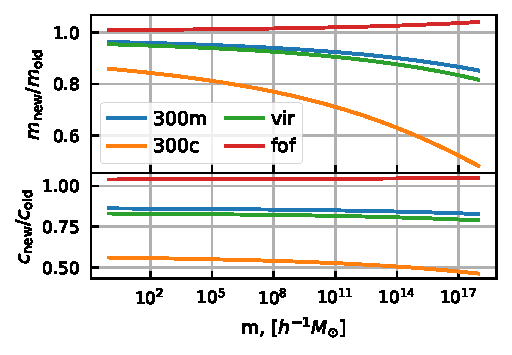
\includegraphics[width=\linewidth]{figures/mass_conversion.pdf}
  \caption[Mass conversion]{Conversion of mass and concentration between different halo definitions. Top-panel shows ratio of converted mass to input mass, as a function of input mass. Different colors represent different halo definitions. Bottom panel shows ratio of converted
  concentration to input concentration, as a function of input mass.
  Input mass definition is 200m. Note that the trend with increasing overdensity is to decrease both the mass and concentration. 
  The halo profile used in the conversion is the NFW profile, and the concentration-mass relation is the simple power law of \cite{Duffy2008}.}
  \label{fig:mass_conversion}
\end{figure}

\subsubsection{Window functions/Filters}
\label{sec:halomod:components:window}
The window/filter function contributes to the basic unit of the spherical collapse formalism, the peak-height $\nu$. It is also responsible for the conversion of distance scales to mass scales (cf. \S\ref{sec:theory:filter}).

Our general approach in this component is to specify all the quantities in terms of the Fourier co-ordinate, $k$, and the smoothing scale $R$. The class itself defines the relationship between mass $m$ and the smoothing scale. The primary quantity of interest is the window function itself, specified in Fourier space, $W(x)$ (one can optionally specify the real-space version as well, though it is not involved in typical HM calculations). With this function, the mass variance can be calculated using Eq. \ref{eq:massvariance}. 

To calculate $dn/dm$ requires also the logarithmic derivative of the variance with mass. To remain as general as possible, we use the following identity
\begin{equation}
    \label{eq:dlnssdlnm}
     \frac{d \ln \sigma}{d \ln m} \equiv \frac{1}{2}\frac{d \ln \sigma^2}{d \ln R} \frac{d \ln R}{d \ln m},
\end{equation}
where 
\begin{equation}
    \label{eq:dlnssdlnr}
    \frac{d\ln \sigma^2}{d\ln R} = \frac{1}{\pi^2 \sigma^2}\int W(kR) \frac{dW(kR)}{d\ln (kR)} P(k) k^2 dk.
\end{equation}
The factor $d\ln R/d\ln m$ is typically 1/3, though this is not necessarily the case for window functions of arbitrary shape\footnote{The mass referenced here is the mass within a shaped volume defined by the window function.} \citep{Schneider2013}. Thus, the defining quantity is the derivative of the window function, $dW(x)/dx$. 

%Table \ref{tab:component_window} summarises our approach to this important quantity. 
We also note that we generalise the calculation of the mass variance to all moments of the smoothed density field:
\begin{equation}
    \label{eq:moments}
    \sigma_n^2(r) = \frac{1}{2\pi^2}\int k^{2n} P(k) W^2(kR) dk,
\end{equation}
for which $\sigma_0^2$ is the usual mass variance.

Table \ref{tab:models_window} summarises the window functions included in \textsc{halomod}, while figure \ref{fig:filter_sigma} displays the value of $\sigma(m)$ for each. Note that there is a complex interplay between the role of $W(kR)$ and the mass assignment which drives changes between the models. Note also that details for \texttt{SharpKEllipsoid} can be found in Appendix A of \cite{Schneider2013}.

\begin{figure}
  \centering
  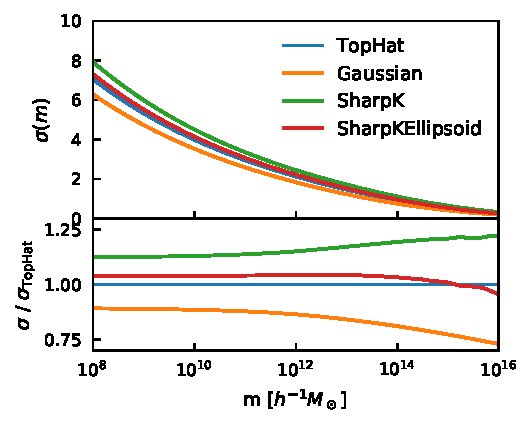
\includegraphics[width=\linewidth]{figures/filter_models.pdf}
  \caption[Mass variance using three different filters]{The mass variance determined by the three most common window functions. The normalisation of the power spectrum in each case uses the \texttt{TopHat} filter, for which $\sigma_8$ is defined.}
  \label{fig:filter_sigma}
\end{figure}

%%%%%%%%%%%%%%%%%%%%%%%%%%%%%%%%%%%%%%%%%%%%%%%%%%%%%%%%%%%%%%%
% \begin{table*}
% \centering
%  {\tabulinesep=1.3mm
% \begin{tabu}{X[1l]X[2l]X[5l]} 
% \toprule[0.05cm]
% \textbf{Available} &  $\bar{\rho}$, $\delta_c$, $k$, $P(k)$ &  \\
% \midrule
% \multirow{3}{*}{\textbf{Required}}  & \texttt{k\_space(kr)} & Fourier-transform of the filter \\
%   & \texttt{dw\_dlnkr(kr)} & The derivative of the Fourier-transform of the filter w.r.t $kr$. \\
%   & \texttt{mass\_to\_radius(m)} & Inverse of mass assignment \\
% \midrule

% \multirow{3}{*}{\textbf{Optional}} & \texttt{dlnr\_dlnm} & Dependence of scale on mass. Required if  relationship is not default: 1/3. \\
%  & \texttt{real\_space(R,r)} & Real-space window function at $r$, with scale $R$. Unnecessary for HM calculations. \\
%   & \texttt{radius\_to\_mass(r)} & Assignment of scale to mass. Unnecessary for HM calculations. Can be supplied for completeness. \\
% \midrule

% \multirow{4}{*}{\textbf{Extra}} & \texttt{dlnss\_dlnr(r)} &  $\frac{d \ln \sigma^2(r)}{d\ln r}$, Eq. \ref{eq:dlnssdlnr} \\
% & \texttt{dlnss\_dlnm(r)} & $\frac{d \ln \sigma^2(r)}{d\ln m}$, Eq. \ref{eq:dlnssdlnm} \\
% & \texttt{sigma(r,order=0)} & Moments of the power spectrum, given by \texttt{order}. Default is $\sigma(r)$. \\
% & \texttt{nu(r)} & Peak-height \\
% \bottomrule[0.05cm]
% \end{tabu}}
% \caption{API summary of the \texttt{Filter} component.}
% \label{tab:component_window}
% \end{table*}
%%%%%%%%%%%%%%%%%%%%%%%%%%%%%%%%%%%%%%%%%%%%%%%%%%%%%%%%%%%%%%%


%%%%%%%%%%%%%%%%%%%%%%%%%%%%%%%%%%%%%%%%%%%%%%%%%%%%%%%%%%%%%%%
\begin{table}
\centering
 {\tabulinesep=1.3mm
\begin{tabu}{X[1.1l]X[2.4l]} 
\toprule[0.05cm]
\textsc{Name} & \textsc{Formula}  \\
\midrule[0.05cm]

\multirow{4}{*}{\texttt{TopHat}}  & $\displaystyle W(r,R) = H(R-r)$ \\
 & $\displaystyle W(x=kR) = \frac{3}{x^3}\left(\sin x - x \cos x\right)$  \\
 & $\displaystyle m(R) = \frac{4\pi}{3}R^3 \bar{\rho}$ \\
 & $\displaystyle \frac{d W}{d \ln x} = \frac{9  x \cos x + 3 (x^2 - 3)  \sin x) }{ x ^3}$  \\
\midrule

\multirow{5}{*}{\texttt{SharpK}}  & $\displaystyle W(r,R) = \frac{\sin(r/R) - (r/R)\cos(r/R)}{2\pi^2 r^3}$   \\
 & $\displaystyle W(x=kR) = H(kR -1)$ \\
 & $\displaystyle m(R) = \frac{4\pi}{3}\left[cR\right]^3 \bar{\rho}$   \\
 & $\displaystyle \frac{d W}{d \ln x} = \delta_D(x-1)$  \\
 & $\displaystyle \frac{d \ln \sigma^2(r)}{d\ln r} = -\frac{P(1/r)}{2\pi^2 \sigma^2(r) r^3} $  \\
 \midrule
 
\multirow{1}{*}{\texttt{SharpKEllipsoid}}  & Same as \texttt{SharpK} except $m(R)$.  \\
\midrule

\multirow{4}{*}{\texttt{Gaussian}}  & $\displaystyle W(r,R) = \frac{\exp(-r^2/2R^2)}{(2\pi)^{3/2} R^3}$  \\
 & $\displaystyle W(x=kR) = \exp(-x^2/2)$ \\
 & $\displaystyle m(R) = (2\pi)^{3/2}R^3 \bar{\rho}$  \\
 & $\displaystyle \frac{d W}{d \ln x} = -xW(x)$  \\


\bottomrule[0.05cm]
\end{tabu}}
\caption[Summary of included \texttt{Filter} models]{Summary of included \texttt{Filter} models. Note: $H$ is the Heaviside step-function, $\delta_D$ is the Dirac-delta function and $P$ is the power spectrum. Also, in \texttt{SharpK}, the mass-assignment is not well-defined, but we use the given formula with $c\approx2.5$ a fit to simulations \protect\citep{Benson2012,Schneider2013}.}
\label{tab:models_window}
\end{table}
%%%%%%%%%%%%%%%%%%%%%%%%%%%%%%%%%%%%%%%%%%%%%%%%%%%%%%%%%%%%%%%

\subsubsection{HMF}
\label{sec:halomod:components:hmf}
The diversity among fitting functions for the HMF, not only in functional forms, but in general approach and explicit parameter dependence, requires that quite a number of variables be available in the general case. However, the typical fit uses just $\nu$ (or sometimes $\sigma$) and its own model parameters, reflecting the expected universality of the fit. 

%To enhance consistency, wherever possible, we reformulate the functions in terms of $\nu$, which is required by the peak-background split arguments to generate a bias function. In cases where the original formulation was in terms of $\sigma$, the quoted parameters will be modified. Of course, in the original, a change in $\delta_c$ (which is often neglected, but happens with changes in cosmology) would not affect the fit at all, whereas in the new it will. The extent of this effect will be very small, and it is unlikely in most applications that $\delta_c$ will modified from its default value of 1.686.
%
%We also provide a mechanism whereby each fit may specify a ``mask", which limits the final result to the mass range that was fit to simulations. This mask is applied at user discretion. 

We present a small selection of 7 out of the 21 available fitting functions available in \textsc{hmf} in Figure \ref{fig:mfs}.
%%%%%%%%%%%%%%%%%%%%%%%%%%%%%%%%%%%%%%%%%%%%%%%%%%%%%%%%%%%%%%%
% \begin{table*}
% \centering
%  {\tabulinesep=1.3mm
% \begin{tabu}{X[1l]X[1.5l]X[2l]} 
% \toprule[0.05cm]
% \textbf{Available} &  $m$, $\nu$, $\delta_c$, $\sigma$, $n_\text{eff}$, $\ln\sigma^{-1}$, $z$, $\Delta_h$, \texttt{cosmo}, $\Omega_m(z)$ &  \\
% \midrule
% \textbf{Required} & \texttt{fsigma(cut\_fit)} & Returns $f(\sigma) \equiv \sqrt{\nu} f(\nu)$, and \texttt{cut\_fit} specifies whether to truncate in the mass range of the fit. \\
% \midrule
% \textbf{Extra} & None & \\
% \bottomrule[0.05cm]
% \end{tabu}}
% \caption{API summary of the \texttt{FittingFunction} component.}
% \label{tab:component_hmf}
% \end{table*}
%%%%%%%%%%%%%%%%%%%%%%%%%%%%%%%%%%%%%%%%%%%%%%%%%%%%%%%%%%%%%%%
We refer the reader to \cite{Murray2013a} for a table of included fitting functions, noting that five more fits have been added to the collection, specifically those of \citet{Tinker2010,Behroozi2013a,Manera2010,Pillepich2010} and \citet{Ishiyama2015}. 

% {\color{red} I would like to add a paragraph here about how to convert $dn/dm$ between mass definitions, if it's a good idea (otherwise, I'd like to take it out of the code!). Would be great to get Benedikt's help on this. Thoughts: this is only useful to take the dndm from the \textit{measured} definition to the input definition. However, I'm not convinced that this is a reasonable thing to do.}
% \bd{I still think it's a somewhat iffy thing to do because of the steep fall-off of the mass function at high mass. My guess is that the solution will essentially suffer from strong Eddington bias, i.e., that convolving one mass function with a no-scatter mdef relation will lead to a MF that differs from the true one for the second distribution. On the other hand, if it could be done, it'd be very powerful.
% My first test would be to take a Tinker+08 MF for, say, 500c, and convolve it with the converion to 200m (so fairly extreme thresholds). Does it come out at all like the Tinker+ MF for 200m?}


\subsubsection{Bias}
\label{sec:halomod:components:bias}
Though the majority of bias functions are specified in `universal' form with respect to the peak-height, there are some older functions that explicitly require cosmology and are specified in terms of a scaled mass, $m/M_\star$. We thus provide access to these quantities, which may also serve to enable more fine-tuned models than possible with pure peak-background split arguments in the future. 

Table \ref{tab:models_bias} compiles the range of included models, and Figure \ref{fig:bias_functions} displays a selection of them.
Note that \halomod\ defines an explicit interface with \textsc{colossus}, enabling all of its bias models to be used in \halomod, including those of \cite{Bhattacharya2011} and \cite{Comparat2017}, which are not included directly in \halomod.

%%%%%%%%%%%%%%%%%%%%%%%%%%%%%%%%%%%%%%%%%%%%%%%%%%%%%%%%%%%%%%%
% \begin{table}
% \centering
%  {\tabulinesep=1.3mm
% \begin{tabu}{X[1l]X[1.5l]X[2l]} 
% \toprule[0.05cm]
% \textbf{Available} &  $m$, $\nu$, $\delta_c$, $\Delta_h$, $\Omega_m$, $n_s$, $M_\star$,$h$, $\sigma_8$ & Note that most of these parameters are unnecessary for most fits. \\
% \midrule
% \textbf{Required} & \texttt{bias()} & Return the bias corresponding to $\nu$ (or equivalently $m$). \\
% \midrule
% \textbf{Extra} & None & \\
% \bottomrule[0.05cm]
% \end{tabu}}
% \caption{API summary of the \texttt{Bias} component.}
% \label{tab:component_bias}
% \end{table}
%%%%%%%%%%%%%%%%%%%%%%%%%%%%%%%%%%%%%%%%%%%%%%%%%%%%%%%%%%%%%%%

\begingroup
 \small
%%%%%%%%%%%%%%%%%%%%%%%%%%%%%%%%%%%%%%%%%%%%%%%%%%%%%%%%%%%%%%%%%%%%
%% BIAS TABLE
%%%%%%%%%%%%%%%%%%%%%%%%%%%%%%%%%%%%%%%%%%%%%%%%%%%%%%%%%%%%%%%%%%%%
\begin{table*} 
\centering

\begin{tabular}{>{\raggedright}m{3cm} >{\raggedright}m{2.6cm} >{\raggedright}m{5.2cm} >{\raggedright\arraybackslash}m{4.2cm} >{\raggedright\arraybackslash}m{1.2cm}}
\toprule
 \textsc{Ref} & \textsc{Name} & \textsc{Formula} & \textsc{Params} & \textsc{hmf}\\
\toprule
 
 \citet{Mo1996} & \texttt{Mo96} & $\displaystyle 1 + \frac{\nu - 1}{\delta_c}$ &  & \texttt{PS} \\
 \midrule
 \citet{Jing1998} & \texttt{Jing98} & $\displaystyle (a/x^2 +1)^{b-cn_s} \left(1 + \frac{x-1}{\delta_c}\right)$ & $x = (m/M_\star)^2$, $a=0.5$, $b=0.06$, $c=0.02$ & \\
 \midrule
 
 \citet{Sheth1999} & \texttt{ST99} & \multirow{2}{*}{$\displaystyle 1 + \frac{q\nu -1}{\delta_c} + \frac{2p/\delta_c}{1+(q\nu)^p}$} & $q=0.707$, $p=0.3$ & \multirow{2}{*}{\texttt{SMT} }\\
\citet{Mandelbaum2005} & \texttt{Mandelbaum05} & & $q=0.73$, $p=0.15$ & \\
\citet{Manera2010} & \texttt{Manera10} & & $q=0.709$, $p=0.248$ & \\
\midrule

\citet{Sheth2001} &\texttt{SMT01} & \multirow{2}{*} { \pbox{20cm}{$\displaystyle  1 +\frac{1}{\sqrt{a}\delta_c}\bigg[s\sqrt{a}(a\nu)+\sqrt{a}b(a\nu)^{1-c}$ \\
$\displaystyle \hphantom{1 +}-\left.\frac{(a\nu)^c}{(a\nu)^c + b(1-c)(1-c/2)}\right]$}} & $a=0.707$, $b=0.5$, $c=0.6$ & \multirow{2}{*}{\texttt{SMT}} \\

 \citet{Tinker2005} & \texttt{Tinker05} \phantom{hey there} &  & $a=0.707$, $b=0.35$, $c=0.8$  &\\
 & & & &\\
\midrule

\citet{Seljak2004} & \texttt{Seljak04} & $\displaystyle a + bx^c + \frac{d}{ex+1} + fx^g$ & $x=m/M_\star$, $a=0.53$, $b=0.39$, $c=0.45$, $d=0.13$, $e=40$, $f=5\times10^{-4}$, $g=1.5$ & \\
\midrule
\citet{Seljak2004} & \texttt{Seljak04Cosmo} & $\displaystyle b_\text{Sel} + \log_{10}x \left[a_1(\Omega'_m + n'_s) + a_2(\sigma'_8 + h')\right]$ & $a_1 = 0.4$, $a_2=0.3$ $\Omega'_m=\Omega_m-0.3$, $n'_s = n_s-1$, $\sigma'_8 = \sigma_8-0.9$, $h' = h-0.7$& \\
\midrule
\citet{Pillepich2010} & \texttt{Pillepich10} & $\displaystyle B_0 + B_1\sqrt{\nu} + B_2\nu$ & $B_0=0.647$, $B_1=-0.320$, $B_2=0.568$ & \\
\midrule
 \citet{Tinker2010} & \texttt{Tinker10} & $\displaystyle 1 - A\frac{\nu^{a/2}}{\nu^{a/2} + \delta_c^a} + B\nu^{b/2} + C\nu^{c/2}$ & $A=1+0.24y\exp[-(4/y)^4]$, $a = 0.44 y - 0.88$, $B = 0.183$, $b = 1.5$, $C = 0.019+0.107y+0.19\exp[-(4/y)^4]$, $c = 2.4$, $y=\log_{10}\Delta_h$. &  \\
 \midrule
 \citet{Tinker2010} & \texttt{Tinker10PBsplit} & $\displaystyle 1 + \frac{\gamma\nu-(1+2\eta)}{\delta_c} + \frac{2\phi/\delta_c}{1+(\beta^2\nu)^\phi}$ & Same as $f_\text{Tinker10}$ & \texttt{Tinker10} \\
 \midrule
 & \texttt{UnityBias} & $b(\nu) = 1$ & & \\
 \bottomrule
 \end{tabular}
 \caption[Summary of included \texttt{Bias} models]{Summary of included \texttt{Bias} models. Note that the fit of \texttt{Manera10} is dependent on Friends-of-Friends linking length and redshift, and we give the result for $l = 0.2$ at $z=0$.}
 
\label{tab:models_bias}

\end{table*}
%%%%%%%%%%%%%%%%%%%%%%%%%%%%%%%%%%%%%%%%%%%%%%%%%%%%%%%%%%%%%%%%%%%%%%%%%%%%%%%%%%%%
\endgroup

\subsubsection{Halo Profiles}
\label{sec:halomod:components:profile}
We developed a systematic representation of two-param\-eter universal halo profiles in \S\ref{sec:profilestheory}. Our implementation follows this development closely. There is a richness of predictions available given just the basic profile shape, which makes the class structure of the \verb|Profile| component extremely valuable. We have not yet implemented several generic predictions that may be added in future versions, such as the gravitational potential profile.

The \verb|Profile| component provides a wide range of derived quantities, accessible with a simple definition of the profile shape. To make this more explicit, suppose that one wished to implement a ``cored" NFW, such that the inner density was a constant $\rho_s$. The minimum code that the user must write (remember, this is user-side code, not touching the \halomod\ source) would be:
%\begin{minted}{python}
%from halomod.profiles import Profile
%class CoredNFW(Profile):
%    def f(self,x):
%        return 1./(1 + x*(1+x)**2)
%\end{minted}
\begin{lstlisting}[language=Python]
from halomod.profiles import Profile
class CoredNFW(Profile):
	def f(self,x):
		return 1./(1 + x*(1+x)**2)
\end{lstlisting}
The class itself can then be used directly or passed to any relevant \framework, and all of the necessary quantities will be available. For increased efficiency, it may also be beneficial to analytically define $p(\kappa,c)$, $h(c)$ and even $l(x,c)$ if available. If not specified, these quantities are evaluated via numerical integration (except for $l(x,c)$ -- it is usually more efficient to use an analytic Fourier-transform $u^2(k|m)$ and then use a Hankel transform on the result).

We define our implemented profiles in Table \ref{tab:models_profile}, and show them in and we note that for each, analytic forms have been given wherever possible to improve efficiency. In general it is non-trivial to produce analytic forms for the self-convolution. Fortunately, this can be achieved with the popular NFW profile \citep{Sheth2001a}, as we show in Table \ref{tab:models_profile}. The associated forms for the $T_i$ are
\begin{subequations}
    \label{eq:nfw_t}
    \begin{align}
        T_1 &= \frac{-4(1+a)+2ax(1+2a)+a^2x^2}{2x^2(1+a)^2(2+x)},\\
        T_2 &= \frac{1}{x^2}\ln\left[\frac{(1+a-ax)(1+x)}{1+a}\right], \\
        T_3 &= \frac{\ln(1+x)}{x(2+x)^2}, \\
        T_4 &= \frac{\ln[(1+a)/(ax+a-1)]}{x(2+x)^2}, \\
        T_5 &= \frac{a^2x-2a}{2x(1+a)^2(2+x)}.
    \end{align}
\end{subequations}

\begin{figure*}
    \centering
    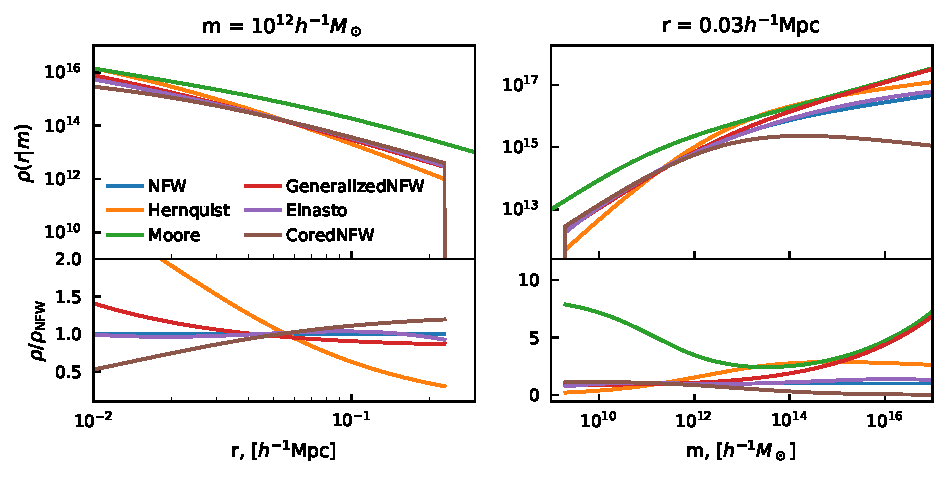
\includegraphics{figures/profile_models.pdf}
    \caption{Illustration of the halo profile models implemented in \texttt{halomod}. Left panel shows the profile as a function of radius at $m=10^{12} h^{-1}M_\odot$, and the right panel shows the profile as a function of mass at $r = 0.03 h^{-1}$Mpc. The general trends are similar, though the inner and outer slopes vary between models. The generalized NFW shown here has $\alpha=1.5$.}
    \label{fig:profiles}
\end{figure*}

For the profile of \citet{Moore1998} and the generalised NFW and Moore profiles, the non-truncated self-convolution can be reduced to a single integral \citep{Ma2000},
\begin{equation}
    l(x) = \frac{2\pi}{x}\int_0^\infty yf(y) F^X_\alpha(x,y) dy,
\end{equation}
where $F$ describes the angular part of the 3D integral. In the case of the generalised NFW, this is fully analytic:
\begin{equation}
    F^N_\alpha(x,y) = \frac{1}{2-\alpha}\left[ \frac{(x+y)^{2-\alpha}}{(1+x+y)^{2-\alpha}} - \frac{|x-y|^{2-\alpha}}{(1+|x-y|)^{2-\alpha}}\right],
\end{equation}
while in the generalised Moore profile, we have
\begin{equation}
    F^M_\alpha(x,y) = \int_{|x-y|}^{x+y} \frac{zdz}{z^p(1+z^{3-\alpha})},
\end{equation}
which for the Moore profile with $\alpha=3/2$ yields
\begin{equation}
    F^M_{3/2} = \frac{1}{3}\left[ 2\sqrt{3} \tan^{-1}\left(\frac{-1+2\sqrt{z}}{\sqrt{3}}\right) + \ln\left(\frac{1+2\sqrt{z} + z}{1-\sqrt{z}+z}\right)\right]\Bigg|_{|x-y|}^{x+y}.
\end{equation}


%%%%%%%%%%%%%%%%%%%%%%%%%%%%%%%%%%%%%%%%%%%%%%%%%%%%%%%%%%%%%%%
% \begin{table*}
% \centering
%  {\tabulinesep=1.3mm
% \begin{tabu}{X[0.8l]X[1.5l]X[2.5l]} 
% \toprule[0.05cm]
% \textbf{Available} &  $\bar{\rho}$, $z$, $\Delta_h$, \texttt{\_cm\_relation} & The \texttt{\_cm\_relation} is a \texttt{CMRelation} model, with relevant methods.  \\
% \midrule
% \textbf{Required} & \texttt{\_f(x)} & $f(x)$, cf. Eq. \ref{eq:universalprofile} \\
% \midrule
% \textbf{Optional} & \texttt{\_l(x,c)} & $l(x,c)$, cf. Eq. \ref{eq:lofxc} \\
% \midrule
% \multirow{10}{*}{\textbf{Extra}} & \texttt{\_h(c)}* & $h(c)$, Eq. \ref{eq:hofc} \\
% & \texttt{\_p(K,c)}* & $p(\kappa,c)$, Eq. \ref{eq:pofck} \\

% & \texttt{\_mvir\_to\_rvir(m)} & $r_\Delta(m)$ \\
% & \texttt{\_rvir\_to\_mvir(r)} & $m_\Delta(r)$ \\

% & \texttt{\_rs\_from\_m(m)}$\dagger$ & $r_s(m)$ \\
% & \texttt{rho(r,m)}$\dagger\ddagger\triangledown$ & $\rho(r|m)$, Eq. \ref{eq:universalprofile}. \\
% & \texttt{lam(r,m)}$\dagger\ddagger\triangledown$ & $\lambda(r|m)$, if \texttt{\_l(x)} is specified.\\
% & \texttt{cdf(r,m)}$\dagger\triangledown$ & Profile CDF, $m(<r)/m_\Delta$ \\
% & \texttt{u(k,m)}$\dagger\ddagger$ & $u(k|m)$, Eq. \ref{eq:uspherical} \\

% & \texttt{\_rho\_s(c)}$\ddagger$ &$\rho_s$, Eq. \ref{eq:hofm} \\

% \bottomrule[0.05cm]
% \end{tabu}}
% \caption[API summary of the \texttt{Profile} component]{API summary of the \texttt{Profile} component. Functions marked by * are pre-defined for free, but for optimization may be specified in subclasses with an analytic form. Functions marked with $\dagger$ have an option of passing $c$ directly instead of $m$. Functions marked with $\ddagger$ are optionally normalised by mass or density. In functions marked with $\triangledown$, the radial coordinate can alternatively be specified as $r/r_s$ or $x$. }
% \label{tab:component_profile}
% \end{table*}
%%%%%%%%%%%%%%%%%%%%%%%%%%%%%%%%%%%%%%%%%%%%%%%%%%%%%%%%%%%%%%%



%%%%%%%%%%%%%%%%%%%%%%%%%%%%%%%%%%%%%%%%%%%%%%%%%%%%%%%%%%%%%%%
\begingroup
\small
\begin{table*} 
\begin{tabular}{ m{4cm} m{12cm}} 
\toprule
\textsc{Name \& Refs.} & \textsc{Formulae} \\
\toprule
\texttt{NFW} & $\displaystyle f(x) = x^{-1}(1+x)^{-2}$ \\
\citet{Navarro1997} & $\displaystyle  h(c) = \frac{c}{1+c} + \ln(1+c)$ \\
\citet{Sheth2001a} & $\displaystyle    p(\kappa,c) = \cos (\kappa) \left(\text{Ci}(c \kappa+\kappa)-\text{Ci}(\kappa)\right) 
                   +\sin (\kappa) \left(\text{Si}(c \kappa+\kappa)-\text{Si}(\kappa)\right)-\frac{\sin (c \kappa)}{c \kappa+\kappa}$ \\
\citet{Ma2000} & $\displaystyle    p(\kappa) =  \frac{1}{2} \left[(\pi -2 \text{Si}|\kappa|) \sin|\kappa|-2 \cos (\kappa) \text{Ci}| \kappa| \right]$ \\
& $\displaystyle  l(x,c) = 4\pi \begin{cases} (T_1 + T_2 +T_3) & 0\leq x \leq c \\
 	(T_4 + T_5) & c\leq x \leq 2c \end{cases}$ \\
 & $\displaystyle l(x) = \frac{8\pi}{x^2(x+2)}\left[\frac{(x^2+2x+2)\ln(1+x)}{x(x+2)} -1 \right]$ \\
 \midrule
 
\texttt{Moore}   &   $\displaystyle f(x) = \frac{1}{x^{3/2}(1+x^{3/2})}$ \\
   \citet{Moore1998}  & $\displaystyle h(c) = \frac{2}{3}\ln \left(c^{3/2}+1\right) $ \\
\citet{Ma2000} & $\displaystyle    p(\kappa) = \frac{G^{7,3}_{3,9}\left(\frac{\kappa^6}{46656}\middle|\frac{1}{12}\left(
\begin{array}{c}
 2,5,11 \\
 2,2,5,6,8,10,11,0,4 \\ 
\end{array}
\right) \right)}{4 \sqrt{3} \pi^{5/2} | \kappa |}$ \\
& $\displaystyle    l(x) = \frac{2\pi}{x}\int_0^\infty  yf(y) F^M_{3/2}(x,y) dy$ \\
\midrule

\texttt{Hernquist}   & $\displaystyle f(x) = \frac{1}{x(1+x)^3}$ \\
  \citet{Hernquist1990} & $\displaystyle  h(c) = \frac{c^2}{2(1+c)^2}$ \\
\citet{Sheth2001a} & $\displaystyle   p(\kappa) = \frac{1}{4} \left[-|\kappa| (2 \text{Ci}|\kappa| \sin|\kappa|+\pi\cos(\kappa)) \right.
    \left.+2\kappa \text{Si}(\kappa) \cos (\kappa)+2\right]$ \\ 
  & $\displaystyle p(\kappa,c) =  1/2 - \frac{\sin (c \kappa)+(c+1)
   \kappa \cos (c \kappa)}{2\kappa(c+1)^2} $ \\
& $\displaystyle \ \ \ \ \ \ \ \ \ 
   + \frac{k}{2} \left[\sin (\kappa) (\text{Ci}(c \kappa+\kappa)-\text{Ci}(\kappa)) \right.
   \left. +\cos (\kappa) (\text{Si}(\kappa)-\text{Si}(c \kappa+\kappa))\right] $\\
  & $\displaystyle  l(x) = \frac{16\pi(h_1 - h_2)}{x^4 * (2 + x)^4} $\\
  & $\displaystyle  h_1(x) = \frac{24 + 60 x + 56 x ^2 + 24x^3 + 6x^4 + x^5}{1 + x} $ \\
  & $\displaystyle  h_2(x) = 12(1 + x)(2 + 2x + x^2)\ln(1 + x) / x$ \\
 \midrule
 
\texttt{GeneralizedNFW} & $\displaystyle    f(x) = \frac{1}{x^\alpha (1+x)^{3-\alpha}}, \ \ \ \  h(c) = -(-c)^\alpha c^{-\alpha}B_{-c}(3-\alpha,\alpha-2)$\\
\citet{Ma2000} & $\displaystyle   p(\kappa) = \frac{2^{-\alpha}}{\sqrt{\pi}\Gamma(3-\alpha)}G^{3,2}_{2,4}\left(\frac{\kappa^2}{4}\middle| {\begin{array}{c}
                      (\alpha-2)/2,(\alpha-1)/2 \\
                        0,0,1/2,-1/2 \\
                    \end{array}}\right) $ \\
& $\displaystyle l(x) = \frac{2\pi}{(2-\alpha)x} \int_0^\infty  yf(y) F^N_\alpha(x,y) dy$ \\
\midrule

\texttt{GeneralizedMoore} & $\displaystyle   f(x) = \frac{1}{x^\alpha (1+x^{3-\alpha})} $\\
\citet{Ma2000} & $\displaystyle    l(x)  = \frac{2\pi}{x}\int_0^\infty  yf(y) F^M_\alpha(x,y) dy $ \\
\midrule

\texttt{Uniform} & $ \displaystyle f(x) = 1, \ \ \ \    h(c) = c^3/3, \ \ \ \  p(\kappa,c) = \frac{\sin(c\kappa) - c\kappa \cos(c\kappa)}{\kappa^3}$\\
\midrule

\texttt{Einasto} & $\displaystyle f(x|\alpha) = \exp\left(-\frac{2(x^\alpha - 1)}{\alpha}\right)$\\
\citet{Einasto1965} & $\displaystyle  h(c|\alpha) = \frac{e^{2 / \alpha}}{\alpha} \left(\frac{2}{\alpha}\right)^{-3/\alpha} \Gamma\left(\frac{3}{\alpha}, \frac{2 c^\alpha}{\alpha}\right)$\\

\bottomrule
\end{tabular}
\caption[Summary of included \texttt{Profile} models]{Summary of included \texttt{Profile} models. Note that for $p$ and $l$, functions explicitly including $c$ are the usual profiles truncated at $r_\Delta$, whereas those that do not explicitly include $c$ are not truncated (these are rather unhelpful in terms of the HM). $G$ is the Meijer-$G$ function. The functions $T_i$ in the NFW definition are found in the text, Eq. \ref{eq:nfw_t}.}
\label{tab:models_profile}
\end{table*}

\endgroup
%\end{onecolumn}
%%%%%%%%%%%%%%%%%%%%%%%%%%%%%%%%%%%%%%%%%%%%%%%%%%%%%%%%%%%%%%%




\subsubsection{Concentration-mass relations}
\label{sec:halomod:components:concentration}
In section \ref{sec:theory:concentration}, we described different classes of models of the $c$--$m$ relation. We have implemented a number of models in \halomod; we summarize them in table \ref{tab:models_concentration} but refer the reader to the respective papers for details.

In particular, we have implemented two age-based models, namely those of \citet{Bullock2001} and \citet{Ludlow2016}. We use interpolating splines to efficiently perform the numerical inversions involved. The results of both models can be approximated with simpler fitting functions, which are also included. Moreover, we add the power-law fits of \citet{Duffy2008} and \citet{Zehavi2011}. 
Note that the power-law fits provided are based on a particular cosmology, and will be inaccurate if used for a model with a different cosmology. Thus, for general purpose applications we recommend an analytic model. 

Figure \ref{fig:concentration} illustrates the variations between the models at $z=0$ for the default cosmology of \cite{PlanckCollaboration2015}. 

Note that \halomod\ includes an explicit interface for using the excellent suite of concentration-mass relations from \textsc{colossus}, which provides access to extra models such as the recent analytical models of \cite{Prada2012} and \cite{Diemer2019}. These models are plotted for comparison in \ref{fig:concentration}, but we do not include them in Table \ref{tab:models_concentration} and refer the reader to their respective papers.


% \bd{Can we include models that are implemented in Colossus? At the moment, the model list for concentration looks a bit random...}

% \bd{what are the weird upturns / downturns in the models in the Figure? Should they really be plotted that far out?}

% \sgm{I put the analytic models from Colossus into the plot, and reduced the mass range plotted (the upturns etc. were from where the analytic models aren't solvable and a constant relation is returned). Do we want to list the colossus models in the table also?}

\begin{figure}
  \centering
  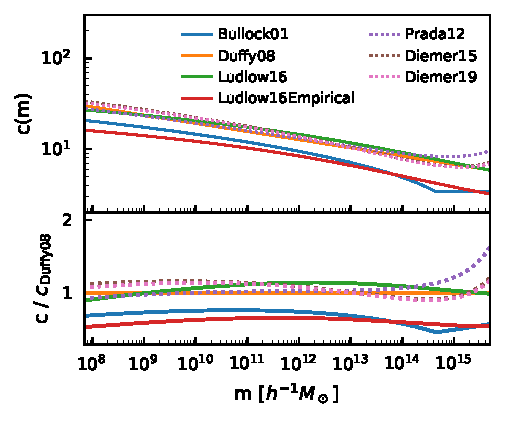
\includegraphics[width=\linewidth]{figures/halo_concentration_models.pdf}
  \caption[Concentration-mass-redshift relation for various models in the literature]{Illustration of the concentration-mass relations implemented in \halomod, focusing on analytic models (with the exception of the class power-law fit of \cite{Duffy2008}). Models plotted with dotted curves are obtained via the explicit interface with \textsc{colossus}, and are able to be used within the entire halo model framework. }
  \label{fig:concentration}
\end{figure}



%The concentration-mass-redshift relation has a diversity of physical models, which makes implementing them in a uniform manner difficult. We begin the process with the most commonly used physical model of \citet{Bullock2001}, and the simple power-law approximations commonly used in observational studies (cf. \S\ref{sec:theory:concentration}).

%The common thread between physical models is the determination of some notion of ``formation time" of a halo \bd{I'd argue that's just one particular class of models...} \sgm{can discuss} -- whether it is the first time a certain fraction of the final mass is assembled, or the typical epoch at which a fraction of the mass collapsed, or some characteristic of the mass accretion history. For analytic models, this is usually obtained via the peak height or some close variant, so the filter function becomes an important quantity in these calculations. 

%Conversely, the power-law approximations generally require nothing more than the model parameters, though we provide the option to calculate the nonlinear mass if it is not passed explicitly.

%Our implementation of the \texttt{Bullock01} model is quite efficient, using interpolated splines to calculate the inverse of the growth factor, in order to acquire the collapse epoch:
%\begin{equation}
%    \label{eq:zc}
%    z_c = D^{-1}(\sqrt{\nu(Fm)}),
%\end{equation}
%where $D$ is the growth factor.

%Similarly, our implementation of the physical model of \citet{Ludlow2016} uses spline interpolation to perform root-finding. We do not present the full equations of that model here, for the sake of brevity, but refer the reader to the decsription in that paper.

%%%%%%%%%%%%%%%%%%%%%%%%%%%%%%%%%%%%%%%%%%%%%%%%%%%%%%%%%%%%%%%
% \begin{table}
% \centering
%  {\tabulinesep=1.3mm
% \begin{tabu}{X[1l]X[1.5l]X[2l]} 
% \toprule[0.05cm]
% \textbf{Available} &  \texttt{filter}, \texttt{growth}, $\bar{\rho}_0$, $\delta_c$, $M_\star(z)$ & The bulk of these quantities will only be required for physical models. $M_\star$ may be passed explicitly as a model parameter, an instance variable, or left to be calculated in the class. \\
% \midrule
% \textbf{Required} & \texttt{cm(m,z)} & Return the concentration corresponding to $m$ at $z$ \\
% \midrule
% \textbf{Extra} & None & \\
% \bottomrule[0.05cm]
% \end{tabu}}
% \caption{API summary of the \texttt{CMRelation} component.}
% \label{tab:component_concentration}
% \end{table}
%%%%%%%%%%%%%%%%%%%%%%%%%%%%%%%%%%%%%%%%%%%%%%%%%%%%%%%%%%%%%%%

%%%%%%%%%%%%%%%%%%%%%%%%%%%%%%%%%%%%%%%%%%%%%%%%%%%%%%%%%%%%%%%%%%%%%%%%%%%%%
\begin{table*}
\centering
\begin{tabu}{X[1.7l]X[1.5l]X[2l]X[3.9l]}
\toprule[0.05cm] 
Ref. & Name & Formula & Params. \\
\toprule[0.05cm]
      
        \citet{Bullock2001} & \texttt{Bullock01} & $\displaystyle K\frac{1+z_c}{1+z}$ & $F=0.001$, $K=3.4$, $z_c$ given in Ref. \\ 
        
        \citet{Ludlow2016} & \texttt{Ludlow16} & See ref. & \\
        \citet{Ludlow2016} & \texttt{Ludlow16Empirical} & $\displaystyle \frac{c_0 (\nu/\nu_0)^{-\gamma_1}}{ \left(1 + \sqrt[\beta]{\nu/\nu_0}\right)^{\beta(\gamma_2 - \gamma_1)}} $ & $c_0 = 3.395(1+z)^{0.215}, \ \ \beta = 0.307(1+z)^{0.54},$ \\
        & & & $\displaystyle \gamma_1 = 0.628(1+z)^{-0.047}, \ \ \gamma_2 = 0.317(1+z)^{-0.893}$\\ 
        \midrule

        \citet{Bullock2001} & \texttt{Bullock01\_Power} & \multirow{3}{*}{$\displaystyle \frac{a}{(1+z)^c}\left(\frac{m}{M_\star}\right)^b$} & $a=9$, $b=-0.13$, $c=1$ \\

        \citet{Duffy2008} & \texttt{Duffy08} & & $a=6.71$, $b=-0.091$, $c=0.44$, $M_\star=2\times10^{12}$ \\

        \citet{Zehavi2011} & \texttt{Zehavi11} & & $a=11$, $b=-0.13$, $c=1$, $M_\star=2.26\times10^{12}$ \\
        
         \bottomrule[0.05cm]
\end{tabu}
\caption{Summary of concentration-mass-redshift relations implemented in \textsc{halomod}. Additional models can be imported from the \textsc{Colossus} code.}
\label{tab:models_concentration}
\end{table*}
%%%%%%%%%%%%%%%%%%%%%%%%%%%%%%%%%%%%%%%%%%%%%%%%%%%%%%%%%%%%%%%%%%%%%%%%%%%%%%%%%%%%


\subsubsection{HOD}
\label{sec:halomod:components:hod}
We keep the implementation of the HOD simple, requiring only the two mean occupation functions for centrals and satellites. Furthermore, there is an optional definition of $m_\text{min}$, which can be used to define a precise lower bound on halo mass. Generally this will be predominantly determined by the parameter $M_\text{min}$, and it defaults to this value if not specified. In general it may be some function of the parameters.

As alluded to in \S\ref{sec:theory-gal:hod}, there is a subtlety in the HOD definition -- the so-called `central condition' -- which is the statement that if no central galaxy exists in a halo in a given sample, then no satellites will be present. Note that the central condition \textit{implies} the statement $\Nc=0 \Rightarrow \Ns=0$, but the reverse is not true in general (one could then still have $\Nc = 0.5$ and $\Ns > 0$, and then a specific halo could still have a satellite but not central). However, if $\Nc$ is a step function from zero to one at some mass (and $\Ns=0$ when $\Nc=0$) then the reverse is true.

The following points outline our approach to this condition:
\begin{enumerate}
    \item The average satellite occupancy is taken to be the average over \textit{all} haloes, with and without centrals. This has subtle implications for how to mock up the galaxy population, because if one requires a central before placing a satellite, then the average number of satellites placed into \textit{available} haloes is increased if the central occupation is less than 1.
    
    \item If the central condition is enforced, then for all HOD classes (except see point 4), the mean satellite occupancy is modified. If the defined occupancy is $\Ns'$, then the returned occupancy is $\Ns = \Nc\Ns'$. This merely ensures that $\Ns=0$ when $\Nc=0$. Note that this will change the interpretation of parameters in the $\Ns$ model, unless $\Nc$ is a simple step function.
    
    \item The pair-wise counts involve a term $\langle N_c N_s\rangle$. When the central condition is enforced, this reduces trivially to $\Ns$. However, if the central condition is not enforced we \textit{assume} that the variates $N_c$ and $N_s$ are uncorrelated, and use $\langle N_c N_s\rangle = \Nc\Ns$.
    
    \item For A HOD class that is defined with the central condition intrinsically \textit{satisfiable} (i.e. $\Ns=0 \Rightarrow \Nc=0$), a variable can be set in the class definition, which will avoid the extra modification of point 2. Note that due to our above observation that being \textit{satisfiable} does not in general imply that it has been \textit{satisfied}, the pairwise counts still depend on whether the user asserts that the central condition is enforced or not (note that in the one case in which \textit{satisfiable} implies \textit{satisfied}, namely a step function $\Nc$, the pairwise counts are the same with or without the central condition).
\end{enumerate}

We present the implemented models in Table \ref{tab:models_hod}. An illustration of the various effects introduced by each HOD is presented in figure \ref{fig:hod}. Note that many of the HOD models are extensions of the more simple models, and are equivalent when setting the extra parameters to zero or one. Typically, \halomod\ will by default render these models the same as the more simple models, with the option of changing the extra parameters.

In addition to the galaxy-focused HOD models presented in Table \ref{tab:models_hod}, \halomod\ provides base classes for diffuse tracers of the underlying DM distribution, such as H\textsc{i} gas. 
In these distributions, it is assumed that there is no distinction between central and satellite, and the only relevant quantity is the mean value of the tracer squared (as a function of mass), which enters the power spectrum integral. 
Furthermore, non-unitless HODs are available in which the occupation can be defined in terms of a \textit{quantity} (eg. H\textsc{i} brightness temperature), but in which that quantity is assumed to be confined to discrete locations within the halos (like galaxies). In these distributions, the central-satellite distinction is maintained.


%%%%%%%%%%%%%%%%%%%%%%%%%%%%%%%%%%%%%%%%%%%%%%%%%%%%%%%%%%%%%%%
% \begin{table}
% \centering
%  {\tabulinesep=1.3mm
% \begin{tabu}{X[1l]X[1.5l]X[2l]} 
% \toprule[0.05cm]
% \textbf{Available} & None &  \\
% \midrule
% \textbf{Required} & \texttt{nc(m)}, \texttt{ns(m)} & Central and satellite mean occupation. \\
% \midrule
% \textbf{Optional} & \texttt{mmin()} & Specification of the minimum possible halo mass. Defaults to $M_\text{min}$. \\
% \textbf{Extra} & \texttt{ntot(m)} & Total mean halo occupation \\
% \bottomrule[0.05cm]
% \end{tabu}}
% \caption{API summary of the \texttt{HOD} component.}
% \label{tab:component_hod}
% \end{table}
%%%%%%%%%%%%%%%%%%%%%%%%%%%%%%%%%%%%%%%%%%%%%%%%%%%%%%%%%%%%%%%

%%%%%%%%%%%%%%%%%%%%%%%%%%%%%%%%%%%%%%%%%%%%%%%%%%%%%%%%%%%%%%%%%%%%%%%%%%%%%%%%%%%%%%
%  HOD Model Table
%%%%%%%%%%%%%%%%%%%%%%%%%%%%%%%%%%%%%%%%%%%%%%%%%%%%%%%%%%%%%%%%%%%%%%%%%%%%%%%%%%%%%%
\begin{table*}
\small
\centering
\begin{tabu}{X[1.7l]X[4l]X[4l]}
\toprule[0.05cm] 
Ref. & $\Nc_m$ & $\Ns_m$ \\
\toprule[0.05cm]
      
        \citet{Zehavi2005} & $H(m-M_\text{min})$ & $\left(\frac{m}{M_1}\right)^\alpha$ \\ \midrule

        \citet{Zheng2005} & $\frac{1}{2}\left[1+\text{erf}\left(\frac{\log m-\log M_{min}}{\sigma_{\log M}}\right)\right]$ & $\left(\frac{m-M_0}{M'_1}\right)^\alpha$ \\ \midrule

        \citet{Tinker2005} & $H(m-M_\text{min})$ & $\exp\left(-\frac{M_\text{cut}}{m-M_\text{min}}\right)\left(\frac{m}{M'_1}\right)H(m-M_\text{min})$ \\ \midrule
                                        
        \citet{Geach2012} & $\begin{aligned}&F_c^B(1-F_c^A)\exp \left[\frac{\log_{10}(m/M_c)^2}{2\sigma^2_{\log M}}\right] \\ &\times F_c^A \left[1+ \text{erf} \left(\frac{\log_{10}(m/M_c)}{\sigma_{\log M}}\right)\right]\end{aligned}$ & $F_s \left[1 + \text{erf} \left(\frac{\log_{10}(m/M_{min})}{\delta_{\log M}}\right)\right]\left(\frac{m}{M_{min}}\right)^\alpha$ \\ \midrule
          
         \citet{Contreras2013} & $N_c^\text{Geach}$, $\sigma_{\log M} \rightarrow x\sigma_{\log M}$ & $N_s^\text{Geach}$ \\
         \bottomrule[0.05cm]
\end{tabu}
\caption[Summary of included HOD parameterisations]{Summary of included HOD parameterisations. Here $H$ is the Heaviside step-function. Note that this table does not include HOD models for diffuse tracers.}
\label{tab:models_hod}
\end{table*}
%$\begin{aligned} &F_c^B(1-F_c^A)\exp \left[\frac{\log_{10}(m/M_c)^2}{2(x\sigma)^2_{\log M}}\right] \\ & \times F_c^A \left[1+ \text{erf} \left(\frac{\log_{10}(m/M_c)}{x\sigma_{\log M}}\right)\right]\end{aligned}$
%%%%%%%%%%%%%%%%%%%%%%%%%%%%%%%%%%%%%%%%%%%%%%%%%%%%%%%%%%%%%%%%%%%%%%%%%%%%%%%%%%%%


\subsubsection{Halo Exclusion}
\label{sec:halomod:components:exclusion}
The primary task of the \verb|Exclusion| component is to evaluate Eq. \ref{eq:dmpower2a} (or Eq. \ref{eq:dmpower2} if appropriate) and the associated (potentially modified) mean density, Eq. \ref{eq:theory:ng_dash}. Each model, as discussed in \S\ref{sec:theory:exclusion}, is quite unique, and therefore there is not a great deal of redundancy that can be mitigate by class inheritance.
Nevertheless, for the sake of consistency, we implement exclusion using the standard \component\ architecture.
%However, each implemented model is segregated into key methods that may provide a basis for extended models. Furthermore, the same classes can be used for either DM or galaxies, since they accept the quantity $I_X$. 

Performance becomes a definite issue with these calculations, especially for those requiring many double-integrations. Thus we introduce alternative methods, where necessary, accelerated by just-in-time compilation using \textsc{numba}. 

We show the effects of the halo exclusion for seven of the implemented models (two of them being modifications to $P_{hh}^c(k)$ rather than physical halo exclusion models) in figure \ref{fig:halo_exclusion}. 
Of these models, it is expected that \verb|DblEllipsoid| and \verb|NgMatched| are the most accurate, and the latter is far more performant.


\subsection{Extra functionality}
\label{sec:halomod:extra}
In addition to the core \framework\ and \component\ elements, we have implemented several pieces of functionality aimed at performing the most commonly required tasks.

\subsubsection{Command-line interface}
\label{sec:halomod:extra:cli}
Though we expect that the vast majority of usage will be interactive or via custom scripts, for additional flexibility we also provide a command-line interface (CLI), which provides a convenient way to compute specified quantities for a range of parameters. This may be useful for batch scripts which only require computation of basic quantities over a large parameter space, or for creating simple interfaces with other programming languages. 

The underlying machinery for the CLI is contained in the \verb|functional| module, which provides a top-level interface for calculating given quantities within a given \framework, for all combinations of a set of given parameters. Due to the homogeneity of the \framework\ definitions, this interface needs only be defined once for all frameworks\footnote{Indeed, due to \halomod\  being inherited from \textsc{hmf}, \halomod\  requires only a thin wrapper around the function in \textsc{hmf} to update some defaults.}. 

The most challenging aspect of this function is the ordering of the implicit loops. As an example, consider a case where the user wishes to range over both redshift and $\Omega_m$ to calculate $n(m)$. It is much more efficient to use redshift as the inner loop, since fewer quantities depend on it, and therefore fewer re-calculations will be performed. This implicit ordering of parameters is accounted for in the routine (if necessary) by performing a very fast low-resolution calculation and determining the number of child quantities for each parameter. This is made possible through the caching system which we have already described (cf. \S\ref{sec:halomod:overview:efficiency}.

Along with the calculated quantities, the routine optionally returns unique labels for each of the iterations, since the return order is not pre-specified.

The CLI wraps this routine, allowing any parameter to be specified by name, either as a scalar or list of values to be iterated over. The CLI ingests a configuration file in \textsc{TOML}\footnote{\url{https://toml.io/en/}} format, but may be over-ridden via command-line arguments. The CLI outputs a complete configuration file (with all default parameters set explicitly) which can be used to re-compute the quantities later. It also outputs each desired quantity in its own file. 


\subsubsection{HOD population}
\label{sec:halomod:extra:pophod}
Quite apart from the analytic formalism outlined in this paper, the HOD allows for creating galaxy catalogues by directly populating halos from $N$-body simulations. Though less efficient than its analytic counterpart, this method is more robust, since it does not depend on approximations for the several halo-based components. Indeed, several authors have used this method, either alone or in conjunction with the analytic calculation \citep{Skibba2015,Zheng2015}. It is also useful as a sanity check.

We provide a very basic set of tools for populating halo catalogues with galaxies using the HOD models included in \textsc{halomod}, synthesised into a CLI. Our implementation assumes a Bernoulli (Poisson) distribution for centrals (satellites), and a spherically symmetric profile for each halo, corresponding precisely to the analytic calculations. It is possible that this functionality will be extended in future versions to account for triaxial profiles \citep{Jing2002} and a range of galaxy classes (such as colour, cf. \citet{Skibba2009}). 



% \subsubsection{Fitting routines}
% \label{sec:halomod:extra:fitting}
% Probably the most common application of the HM in the past decade has been to use the analytic model to fit HOD parameters using observed clustering data. We provide a very flexible interface for this purpose, both as a method and a CLI. 

% Again exploiting the homogeneity of the core \framework\ structure, we are able to present a unified interface to any \framework\ and an arbitrary selection of its properties. The features of the fitting capabilities include:
% \begin{itemize}
%     \item CLI or functional interface
%     \item Fit to any quantity from any any \framework\
%     \item Completely specify the base model parameters (with defaults given by normal usage).
%     \item Arbitrary specification of variable parameters to be fit (including elements of any of the \component\ parameter dictionaries). 
%     \item Several parameter priors , including uniform, log-uniform, normal and multivariate normal distributions.
%     \item Support for independent or covariant Gaussian uncertainties in the measured quantities.
%     \item Extendible system for specifying fitting methods, with Markov Chain Monte Carlo (MCMC) fitting implemented with an Affine-Invariant Ensemble Sampler (provided by the \textsc{emcee}\footnote{\url{dan.iel.fm/emcee/}} package), and downhill-gradient fits using the minimization package in \textsc{scipy}\footnote{\url{http://www.scipy.org/}}.
%     \item Concurrent output of arbitrary properties, useful for identifying distributions of derived quantities (eg. effective bias or mass). 
%     \item CLI interface largely defined by a readable config file.
% \end{itemize}


\section{\textsc{TheHaloMod} web-application}
\label{sec:thehalomod}
\citet{Murray2013a} presented \textsc{HMFcalc}, an online HMF calculator that has since been widely used in the community.
Web-applications can be useful, as they circumvent the overhead of installing custom software and using a command-line or interpreter interface. 
As such, they are more readily employed by researchers seeking to obtain a single model to corroborate the output of a simulation or observation.
Perhaps more interestingly, the intuitive and graphical nature of web-apps make them extremely useful for educational purposes -- whether in a classroom setting, or for self-learning.
It is with these motivations that we present a successor to \textsc{HMFcalc}\footnote{\textsc{HMFcalc} was located at \url{https://hmf.icrar.org}. This address now automatically forwards to the address of \textsc{TheHaloMod}, at \url{https://thehalomod.app}. All the functionality of \textsc{HMFcalc} is available in \textsc{TheHaloMod}.} that computes the full range of halo model quantities we have outlined in this paper -- called \textsc{TheHaloMod}.


\subsection{Interface}
The interface of \thm\ is expansive but simple. The user is presented immediately with a default model, which occupies a central plot. A drop-down menu lets the user select which quantity to view. Using a \halomod\ \verb|TracerHaloModel| on the backend, these quantities are computed on-the-fly and then cached so they can be view again quickly.

Below the plot itself is a table of computed models (consisting of just the default plot at first), each of which has a unique user-provided label. 
The user can remove or edit a model, or create a new model based on any existing model. Editing or model creation bring the user to the same interface containing a rather large input form. 
The form itself is separated into tabs -- one for each \framework, and one for each \component. 
Each \component, in particular, has a drop-down menu for choosing the particular model, and a unique set of input parameters for each model.
Once parameters have been chosen (including the unique label), the user is taken back to the main plot interface, and is free to continue adding and editing models.

The user may also download various pieces of data: the plot itself, a readable list of parameters for each of the models, or data files containing \textit{all} the quantities of the halo model for each model.


\subsection{Architecture}
\thm\ is powered by \textsc{django}\footnote{\url{https://www.djangoproject.com/}} and uses the \textsc{bootstrap}\footnote{\url{https://getbootstrap.com/}} CSS framework and \textsc{jQuery}\footnote{\url{https://jquery.com/}} Javascript library to achieve a reasonable UI with minimal fuss.

Architecturally, \thm\ makes great use of the object-oriented forms in \textsc{django}, in concert with the consistency of all the \texttt{Component}s. 
This consistency means that very few lines of code are required to create separate form tabs for each \component. 

Javascript functionality is kept to a minimum, but provides extremely useful UI improvements in some key cases. 
In particular, each \component\ model has potentially unique parameters. Javascript is used to make only relevant parameters visible to the user, dependent on their current choices. 
It is also used to provide a smooth experience when changing the quantity to be viewed in the plot (i.e. this can occur without reloading the page).

\thm\ is hosted by the Low-Frequency Cosmology (LOCO) Lab at Arizona State University. Deployment is aided by containerizing the entire application using Docker\footnote{\url{https://www.docker.com/}}.



%The Halo Model has become an indispensable tool for cosmological spatial statistics analysis in the past decade. Consequently, its use is becoming more widespread, with interest from those who are not necessarily core to its development. 
%Such a context is an excellent motivation for creating a web-based implementation which is readily available with no installation requirements, and an intuitive interface.
%

%To this end, we have developed \verb|TheHaloMod|, a web-application which exposes much of the functionality of \verb|halomod| in a graphically helpful web-environment. This application is a successor and extension of \verb|HMFcalc|, which provided a similar interface for \verb|hmf|. Therefore, many of the details of the implementation of \verb|TheHaloMod| are equivalent to those for \verb|HMFcalc|, which was described in \citet{Murray2013}. However, several components have been significantly updated in \verb|HMFcalc|, and some extra features have been necessarily added.
%
%\subsection{Updates in HMFcalc}
%The primary development in \verb|HMFcalc| has been the transition to a more object-oriented structure, following more closely the ideology of the \verb|hmf| back-end. 
%The session stores each calculated model as the entire object, rather than a data-table of required quantities. This allows the later access of any quantity from the object without an intermediate step. Furthermore, it allows the deferred calculation of quantities that are not required until the user specifically requests them. This is a major conceptual simplification.
%
%Visually, \verb|HMFcalc| has evolved from a two-page calculator, into a dynamic single-page environment. This transition has been facilitated by a JavaScript plotting library XXX and several JavaScript functions to control the dynamic nature of the page. This environment gives the user more control over the graphical and data output, which in turn enhances the insight to be gained. Among these extra controls is a flexible axis chooser, which enables each axis to be specified from any of the available quantities. Furthermore, each graph can optionally be plotted in log-space, and optionally be a ``comparison" between models (by taking their ratio). 
%
%\verb|TheHaloMod| has similarly been implemented with these improvements.
%
%\subsection{New Features}
%\verb|TheHaloMod| extends \verb|HMFcalc| by introducing all the components necessary for calculating Halo Model quantities, such as the two-point correlation function (cf. \S\ref{sec:HaloModel}). These are introduced as a series of tabs in the input form, each of which delineates a set of parameters corresponding to a different component. 
%
%Also provided is a function for performing a fit to user-uploaded data in a generic and flexible way. This function requires the result to be emailed to the user, as the fit can take a significant period to run.
%
%Furthermore, a function to fill a user-uploaded catalogue of halos with galaxies, following a simplistic HOD model is provided. 


\section{Example Application}
\label{sec:applications}

To illustrate the utility of \halomod\ in semi-realistic applications, we here present a worked example of fitting parameters to mock galaxy data\footnote{The full example notebook can be found at \url{https://halomod.readthedocs.io/en/latest/examples/fitting.html}}. 
We do not use real data, but instead create some simplistic mock data using \halomod\ itself.

We note that we do \textit{not} include native fitting capabilities in \halomod. The reason for this is that applications in constraining parameters, and their relevant likelihoods, are so diverse. It is impossible to capture the range of realistic likelihoods, and it is more useful to let the user adopt one of the many excellent Bayesian (or more general fitting) frameworks in the Python ecosystem\footnote{Examples include \textsc{emcee}, \textsc{PyMC3}, \textsc{PyStan} and \textsc{cobaya}.}.
However, \halomod\ was partially motivated by the desire to perform HOD fits on galaxy data, and it is thus written in a manner conducive to this end.
For instance, each \framework\ is pickle-able by the \verb|dill.pickle| library. 
Furthermore, due to the fact that all quantities of interest are simply obtained by accessing attributes, quite general likelihoods can be written that are able to dynamically switch between different quantities. We will utilise this feature in our example here.

In our example, we will simply create mock data to which we fit a matching HOD model. 
The mock data is generated as $\xi_{gg}(r)$, with diagonal covariance matrix and Gaussian noise at an amplitude of 10\% of the amplitude of the correlation function itself. In addition, we use the constraint of galaxy number density (with a Gaussian uncertainty of $10^-4 h^3{\rm Mpc}^{-3}$) to break a degeneracy in the HOD parameters.
The appropriate likelihood is thus a simple $\chi^2$ between the mock and model $\xi_{gg}(r)$, along with an extra Gaussian term for the mean galaxy number density.

We use \textsc{emcee} to perform the actual Bayesian inference in this example, though it should be clear how to adapt the likelihood to other frameworks. We can write a fairly generic likelihood function:

%\begin{minted}{python}
%def log_prob(
%    param_values: np.ndarray, 
%    param_names: List[str], 
%    data: np.ndarray,
%    model: TracerHaloModel, 
%    derived: Optional[Tuple[str]]=()
%):
%    # Pack parameters into a dict
%    params = dict(zip(param_names, param_values))
%    
%    # Allow for simple bounded flat priors.
%    bounds = bounds or {}
%    for key, val in params.items():
%        bound = bounds.get(key, (-np.inf, np.inf))
%        if not bound[0] < val < bound[1]:
%            return -np.inf, []
%            
%    # Update model with all fitting parameters 
%    params = flat_to_nested_dict(params)
%    model.update(**params)
%
%    # Get arbitrary derived data
%    derived = [getattr(model, d) for d in derived]
%
%    # Calculate chi^2 likelihood
%    logl = chi_square(
%        model=model.corr_auto_tracer, 
%        data=data, 
%        sigma=0.2 * np.abs(model.corr_auto_tracer)
%    )
%    
%    # Return derived to make emcee "blobs"
%    return logl, derived
%\end{minted}
\begin{lstlisting}[language=Python]
def log_prob(
	param_values: np.ndarray, 
	param_names: List[str], 
	data: np.ndarray,
	model: TracerHaloModel, 
	derived: Optional[Tuple[str]]=()
):
	# Pack parameters into a dict
	params = dict(zip(param_names, param_values))

	# Allow for simple bounded flat priors.
	bounds = bounds or {}
	for key, val in params.items():
		bound = bounds.get(key, (-np.inf, np.inf))
		if not bound[0] < val < bound[1]:
			return -np.inf, []

	# Update model with all fitting parameters 
	params = flat_to_nested_dict(params)
	model.update(**params)
	
	# Get arbitrary derived data
	derived = [getattr(model, d) for d in derived]
	
	# Calculate chi^2 likelihood
	logl = chi_square(
		model=model.corr_auto_tracer, 
		data=data, 
		sigma=0.2 * np.abs(model.corr_auto_tracer)
	)
	
	# Return derived to make emcee "blobs"
	return logl, derived
\end{lstlisting}

This function contains a reference to another custom function, \verb|flat_to_nested_dict|, whose purpose is to take a dictionary with 
dot-path keys and convert it to a nested dictionary, so that eg. \texttt{\{'nested.key': 3\}} is converted to \texttt{\{'nested': \{'key': 3\}\}}. This makes it possible set arbitrary parameters of components within the \texttt{Tracer\-Halo\-Model}, as we shall see. 

Furthermore, notice that arbitrary derived data is able to be extracted due to the consistent API of the \framework, in which every quantity is accessed as an attribute. 
Due to the efficient caching system (cf. \S\ref{sec:halomod:overview:efficiency} and \ref{app:caching}), the order in which quantities are accessed is irrelevant, and only the quantities that are required are actually calculated.
We return these arbitrary derived data as a list of \verb|emcee| ``blobs'', so that we can plot posteriors of the derived parameters.

This likelihood function is more than generic enough for this example, and many others, and is a good starting place for most likelihoods that the user might wish to write.
One clear deficiency in the log probability function is the absence of sophisticated priors on the parameters. 
Most sophisticated Bayesian frameworks have abstract mechanisms for defining priors, but \verb|emcee| assumes that the priors will be added to the probability inside the \verb|log_prob| function. 
Due to the non-general nature of such a code, we omit it for these examples, implicitly assuming flat priors on all parameters. 
We do however include a potential bound on each parameter, which should serve as a simple starting point for extensions to more complex priors.

We start the MCMC chains in a small Gaussian ball around the true parameters (or close to the true parameters in the case of the mismatched model) and let them expand to fill the posterior\footnote{This is recommended in the \textsc{emcee} documentation.}. 
The chains have 100 walkers, and comprise 10000 iterations, of which the first 1000 are removed as burnin. 
As this is a toy examples, explicit convergence tests are not performed as they should be in real applications. 

% \subsection{Example 1: Fitting a matching HOD model}
% \label{sec:applications:hod}

Our mock data is created with a default \texttt{Tracer\-Halo\-Model} set at a redshift of $z=0.2$, and using the transfer model of \citet{Eisenstein1998}. The HOD model is \verb|Zehavi05| (cf. Table \ref{tab:models_hod}), with $M_{\rm min} = 10^{12}$, $M_1 = 10^{12.8}$ and $\alpha = 1.05$.

Constraining the parameters is simple. We construct the sampler like so:
%\begin{minted}{python}
%sampler = emcee.EnsembleSampler(
%    nwalkers = 100,
%    ndim = 3,
%    log_prob_fn = log_prob,
%    kwargs = {
%        'param_names': [
%            'hod_params.M_min', 
%            'hod_params.M_1', 
%            'hod_params.alpha'
%        ],  
%        'data': (mock_data, mock_ngal), 
%        'model': model,  
%        'derived': [
%            'satellite_fraction', 
%            'mean_tracer_den',
%            'bias_effective_tracer',
%            'corr_auto_tracer'
%        ],
%    },
%    blobs_dtype=[
%        ("sat_frac", float), 
%        ("tracer_den", float), 
%        ("bias_effective_tracer", float),
%        ("corr_auto_tracer", (float, len(mock_data)))
%    ]
%)
%\end{minted}
\begin{lstlisting}[language=Python]
sampler = emcee.EnsembleSampler(
	nwalkers = 100,
	ndim = 3,
	log_prob_fn = log_prob,
	kwargs = {
		'param_names': [
			'hod_params.M_min', 
			'hod_params.M_1', 
			'hod_params.alpha'
		],  
		'data': (mock_data, mock_ngal), 
		'model': model,  
		'derived': [
			'satellite_fraction', 
			'mean_tracer_den',
			'bias_effective_tracer',
			'corr_auto_tracer'
		],
	},
	blobs_dtype=[
		("sat_frac", float), 
		("tracer_den", float), 
		("bias_effective_tracer", float),
		("corr_auto_tracer", (float, len(mock_data)))
	]
	)
\end{lstlisting}

and then create the initial positions and sample for 10000 iterations:
%\begin{minted}{python}
%initialpos = np.array([
%    fiducial_model.hod.params['M_min'], 
%    fiducial_model.hod.params['M_1'],
%    fiducial_model.hod.params['alpha']
%]) + 1e-4 * np.random.normal(
%    size=(sampler.nwalkers, sampler.ndim)
%)
%
%sampler.run_mcmc(initialpos, nsteps=10000)
%\end{minted}
\begin{lstlisting}[language=Python]
initialpos = np.array([
	fiducial_model.hod.params['M_min'], 
	fiducial_model.hod.params['M_1'],
	fiducial_model.hod.params['alpha']
]) + 1e-4 * np.random.normal(
	size=(sampler.nwalkers, sampler.ndim)
)
	
sampler.run_mcmc(initialpos, nsteps=10000)
\end{lstlisting}
Note that in the setup of the \verb|EnsembleSampler| we have specified the parameters we wish to constrain simply by passing a list of dot-pathed names.
The first part of the name refers to the \parameter\ name in the \framework\ that we would like to update. In this case, \verb|hod_params| is itself a dictionary of parameters for the HOD, and so the second part of the dot-path is the name of the parameter within that dictionary. This makes it possible to constrain any continuous parameter defined at any level of the framework.

Note also that the \verb|model| variable is itself a \texttt{Tracer\-Halo\-Model} instance, cloned from the original fiducial model from which we created the \verb|mock_data| using the simple command \texttt{model = fid\_model.clone()}. 
This \verb|model| is mutable and is internally updated in the \verb|log_prob| function, so it is useful to keep the original fiducial model untouched.

After removing burnin and thinning by every $5^{th}$ sample to reduce correlations, we can make Fig. \ref{fig:example1_corner}, which shows that that parameters were recovered with moderate accuracy. 
Note that in this ``corner plot'', we have also shown the joint posteriors of the three derived scalars -- the satellite fraction, the mean galaxy density and the linear galaxy bias.  

Furthermore, Fig \ref{fig:example_resids} shows the posterior 68\%  percentile range of the correlation function, along with the ratio of the mock data to the median. The posterior of the model $\xi(r)$ is here easily obtained from the output sampler: \texttt{sampler.get\_blobs(flat=True)['corr\_auto\_tracer']}. \\
Notice that the residuals are noise-like, as is expected from this toy model.

\begin{figure*}
    \centering
    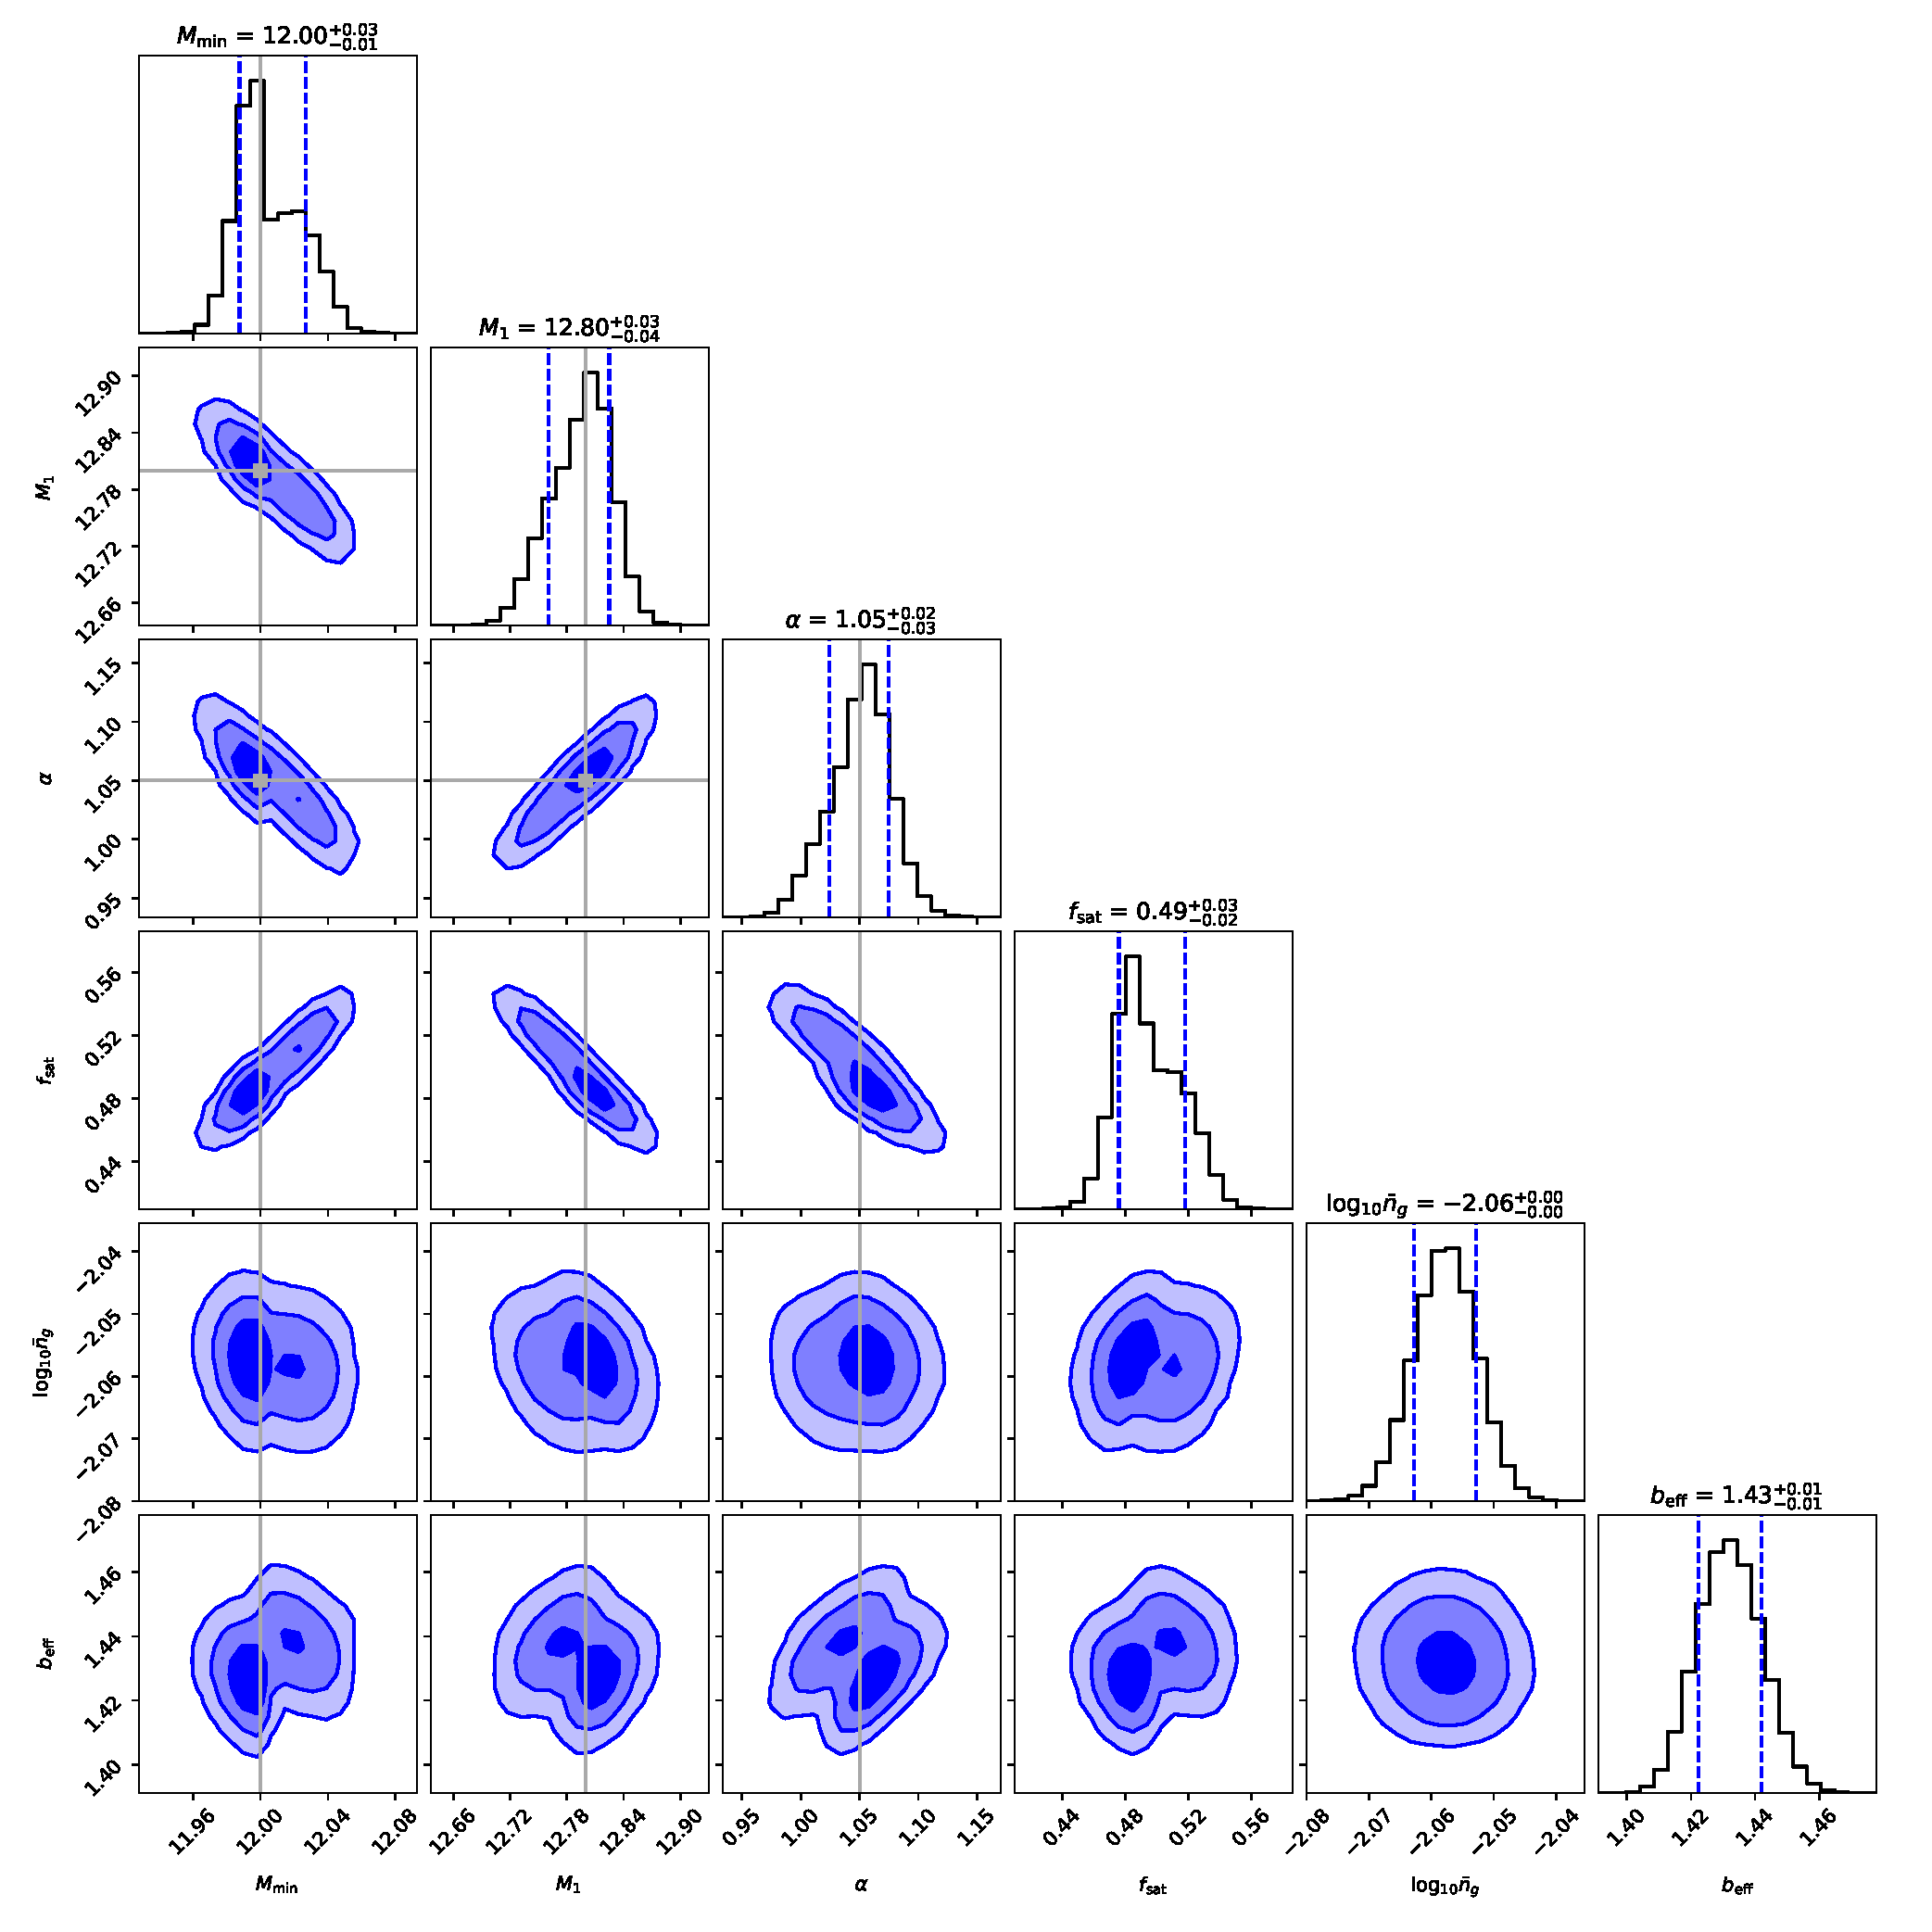
\includegraphics[width=\textwidth]{figures/default_corner.pdf}
    \caption{Corner-plot showing joint posteriors for each of the three HOD parameters, as well as the three derived parameters (satellite fraction, mean galaxy number density and linear galaxy bias). Example code to reproduce this plot is found throughout \S\ref{sec:applications}. }
    \label{fig:example1_corner}
\end{figure*}

\begin{figure}
    \centering
    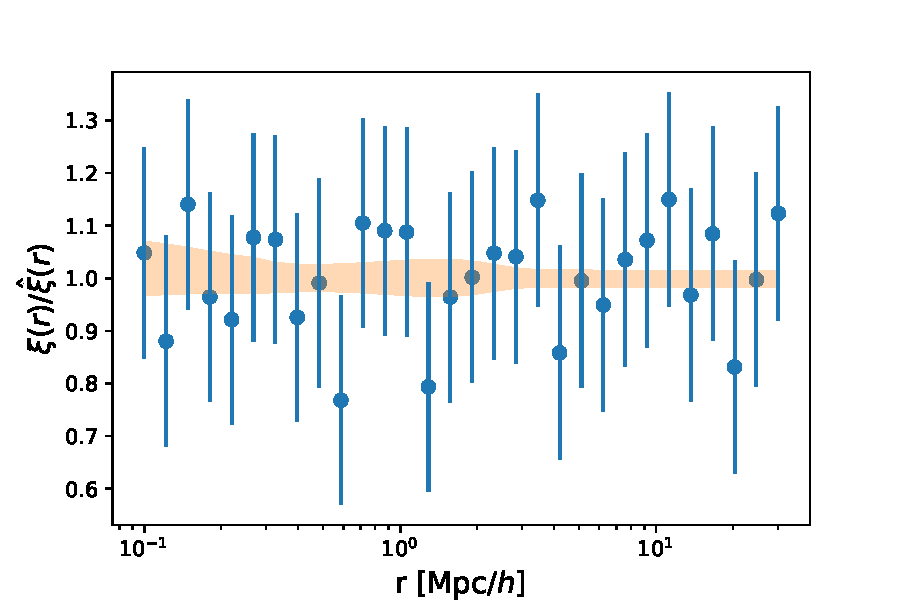
\includegraphics[width=\linewidth]{figures/residuals.pdf}
    \caption{Ratio of mock data to the median posterior of $\xi(r)$. Here, the median posterior is calculated as the median (per $r$-bin) of the posterior \textit{samples} (not the model at the median of the posterior of the parameters). Error-bars shown are 10\% uncertainties as input to the mock data. The orange region is the 68\% central quantile of the posterior. The residuals are noise-like.}
    \label{fig:example_resids}
\end{figure}

It is easy to imagine extensions to this example -- using projected or angular correlation functions, more sophisticated HOD models, allowing cosmology to be free, or using multiple datasets simultaneously. 
In most cases, the necessary modifications to the example code presented here will be small, illustrating the simplicity and flexibility of \halomod.


% \subsection{Example 2: Fitting Non-HOD parameters}
% \label{sec:applications:nonhod}

% In this example, we retain the HOD parameters from the previous example, but also attempt to fit two cosmological parameters: $\sigma_8$ and the spectral index $n_s$. 
% Since we expect these to be poorly constrained by the observation, but highly constrained by priors from the CMB, we set fairly tight prior ranges on them.
% The call to \verb|EnsembleSampler| remains almost exactly the same, except that \verb|'sigma_8'| and \verb|'n'| are added to the \verb|param_names|, \verb|ndim| is increased to 5, and we set \mintinline[breaklines,breakafter=:]{python}|bounds={"sigma_8":(0.75,0.85), "n":(0.94, 1.02)}|.

% We show the resulting corner plot, this time omitting the derived scalar parameters for clarity, in Fig. \ref{fig:example2_corner}. {\color{red} COMMENTS}. The residual plot is shown in \ref{fig:example_resids}.

% \subsection{Example 3: Non-Matched Model}
% \label{sec:applications:non-matched}

% In this example, we again retain the HOD parameters from the first example, but we assume that the profile model is the form of \citet{Einasto1965} (cf. Table \ref{tab:models_profile} and Fig. \ref{fig:profiles}). This profile is able to fit the NFW form quite closely, but not exactly, using $\alpha_{\rm Ein}\sim 0.18$. 

% We let this parameter vary during the fit in this example, effectively using the galaxy correlation function inform us about the halo profile shape. We do not expect tight constraints on $\alpha_{\rm Ein}$, as systematic effects from the uncertain HOD parameters will be dominant. Thus, we set a reasonably tight prior on $\alpha_{\rm Ein}$ to avoid numerical issues, in particular we set \mintinline[breaklines,breakafter=:]{python}|bounds={'halo_profile_params.alpha':(0.05, 0.4)}| in the constructor to \verb|EnsembleSampler|. 

% We show the resulting corner plot, this time omitting the derived scalar parameters for clarity, in Fig. \ref{fig:example3_corner}. {\color{red} COMMENTS}. The residual plot is shown in \ref{fig:example_resids}.

% To illustrate the utility of \textsc{halomod} for common halo model applications, we here present an example motivated by typical analyses. In particular, we fit HOD models to the observed projected correlation function from the 6-degree Field Galaxy Survey \citep[6dFGS;][]{Jones2009}, in much the same fashion as the analysis in \citet[hereafter B13]{Beutler2013}\footnote{It must be noted that the observed correlation functions and their covariance matrices were kindly provided by Florian Beutler.}. 

% \subsection{Setup and methodology}
% Our aim is to begin by performing the same basic analysis as B13 (in a limited sense), but then extend it somewhat to show the flexibility of \halomod\  . Thus, we use the closest sample from their analysis, called ``S1", which has a mean redshift of $z=0.0369$ and mean density of $4.536\times10^{-3} h^3 \text{Mpc}^{-3}$, and use the inbuilt MCMC capabilities of \halomod\  to fit increasingly complex sets of variables with it. 

% In all cases, we use the measured $w_p(r_p)$ from S1, with errors given by a covariance matrix measured with jack-knife resampling. We also use the mean galaxy density as a measurement to be fit, with a 1\% uncertainty.

% All of our chains contain $10^5$ samples before the removal of burn-in, generated with 100 ensemble walkers. Burn-in length is determined by spectral methods, as 5 times the maximum autocorrelation length. The time-per-sample required for the runs on a standard quad-core machine running two cores per chain ranges from 1/40 to 1/10 seconds depending on the variables involved. 

% In contrast to B13, we use the more recent cosmological parameter set of \cite[hereafter P15]{PlanckCollaboration2015}, which is built-in to \halomod\  \footnote{Note that the observable will have insignificant variation with cosmology due to the very low mean redshift of the sample.}. Furthermore, we use the HMF and bias models of \citet{Tinker2010}, and for simplicity, we use the transfer function of \citet{Eisenstein1998}. A concise summary of our base model is found in table \ref{tab:base_model}, which also highlights settings that differ from B13. 

% \begin{table}
%     \centering
%     \begin{tabu} {X[3l]X[2l]}
%         \toprule[0.05cm] 
%         \textsc{Parameter} & \textsc{Value}  \\
%         \toprule[0.05cm]
        
%         Cosmology*, $\sqrt{\nu}f(\nu)$*, $b(\nu)$, $c(m,z)$ & See table \ref{tab:mcmc_variables} \\
%         $T(k)$* & \texttt{EH} \\
%         $S(\xi_m(r))$ & \texttt{Tinker\_SD05} \\
%         $\rho(r|m)$ & NFW \\
%         \texttt{exclusion\_model} & \texttt{NgMatched\_} \\
%         \midrule
        
%         \texttt{lnk\_min}, \texttt{lnk\_max}, \texttt{dlnk} & -4, 2, 0.02 \\
%         \texttt{dlog10m} & 0.04 \\
%         \texttt{rnum} & 50 \\
%         \midrule 
                
%         \texttt{proj\_limit} & 50.0 \\
%         \texttt{z} & 0.0369 \\
%         \texttt{hc\_spectrum} & Nonlinear \\
%         \texttt{takahashi} & True \\    
%         \bottomrule[0.05cm]
%     \end{tabu}
%     \caption[Summary of base model for MCMC runs in example application]{Base model for our MCMC runs. The top section lists the various models used, the middle section lists the accuracy parameters, and the bottom section some extra options (some sample-specific). Note that the accuracy parameters were chosen to be as coarse as possible while only inducing a $<1\%$ error at any scale. Parameters marked with an asterisk (*) are known to differ from the analysis of B13.}
%     \label{tab:base_model}
% \end{table}

% %%%%%%%%%%%%%%%%%%%%%%%%%%%%%%%%%%%%%%%%%%%%%%%%%%%%%%%%%%%%%%%%%%%%%%%%%%%%%
% %  MCMC parameter table
% %%%%%%%%%%%%%%%%%%%%%%%%%%%%%%%%%%%%%%%%%%%%%%%%%%%%%%%%%%%%%%%%%%%%%%%%%%%%%
% \begin{table*}
%     \centering
%     \begin{tabu} {X[2l]X[2l]X[1l]X[4l]}
%         \toprule[0.05cm] 
%         \textsc{Param} & \textsc{Prior} & \textsc{Baseline} & \textsc{Description} \\
%         \toprule[0.05cm]

%         \multicolumn{3}{l}{\textsc{HOD}}    \\
%         $M_\text{min}$ & $[10,14]$ & & Minimum halo mass containing galaxies. \\
%         $M_1$ & $[10.85,15.2]$ & & Halo mass on average containing one satellite. \\
%         $\alpha$ &   $[0.5,1.7]$ & & Growth index of satellite occupation with halo mass \\
%         \midrule
        
%         \multicolumn{3}{l}{\textsc{Cosmology}*}    \\
%         $\sigma_8$ & $[0.4,1.1]$ & 0.846 & RMS density within spheres of 8$h^{-1}$Mpc \\
%         $n_s$ & $[0.7,1.3]$ & 0.9669  & Spectral index. \\
%         $\Omega_m$ &   $[0.2,0.4]$ & 0.3114 & Matter density today divided by critical density \\
%         $\Omega_b$ &   $[0.025,0.075]$ & 0.04888 & Baryon density today divided by critical density \\
%         $H_0$ & $[55.0,85.0]$ & 67.58 & Hubble constant today. \\
%         \midrule
        
%         \multicolumn{3}{l}{\textsc{HMF}}    \\
%         $\alpha_0$ & \multirow{5}{*}{$\mathcal{N}(\mu,10\%)$} & 0.368 & \multirow{5}{*}{\parbox{5.5cm}{$z=0$ parameters of the \citet{Tinker2010} fit.}} \\
%         $\beta_0$ & & 0.589 & \\
%         $\gamma_0$ & & 0.864 & \\
%         $\phi_0$ & & -0.729 & \\
%         $\eta_0$ & & -0.243 & \\        
%         \midrule 
        
%         \multicolumn{3}{l}{\textsc{Bias}}    \\
%         $B$ & \multirow{3}{*}{$\mathcal{N}(\mu,10\%)$} & 0.183 & \multirow{3}{*}{\parbox{5.5cm}{$z=0$ parameters of the \citet{Tinker2010} bias.}} \\
%         $b$ & & 1.5 & \\
%         $c$ & & 2.4 & \\
%         \midrule        

%         \multicolumn{3}{l}{\textsc{Concentration}}
        
        
%         \\
%         $a$ & \multirow{3}{*}{$\mathcal{N}(\mu,10\%)$} & 6.71 & \multirow{3}{*}{\parbox{5.5cm}{Parameters of the \citet{Duffy2008} $c(m,z)$ relation}} \\
%         $b$ & & -0.091 & \\
%         $c$ & & 0.44 & \\
        
%         \bottomrule[0.05cm]
%     \end{tabu}
%     \caption[Summary of the variable parameters used in MCMC runs]{Summary of the variable parameters used in MCMC runs in \S\ref{sec:applications}. Listed are the parameter symbols (delineated by component), prior range, base value (in runs where it is not varied), and a description. In some runs, we impose a multivariate Gaussian prior on the cosmological variables, derived from the MCMC chains from P15. Furthermore, when we vary only $\sigma_8$, it takes a normal prior based on these same chains. The mean of these chains is the value listed in the baseline column. The HMF, bias and concentration parameters receive a normal prior, with 10\% width and mean given in the baseline column. \bd{Is this table a default? It says ``used in MCMC runs'' but surely these params vary?}}
%     \label{tab:mcmc_variables}
% \end{table*}
% %%%%%%%%%%%%%%%%%%%%%%%%%%%%%%%%%%%%%%%%%%%%%%%%%%%%%%%%%%%%%%%%%%%%%%%%%%%%%

% \subsection{Results}
% Our first task is to re-perform the analysis of B13, which varies only the HOD parameters. Figure \ref{fig:typical} shows the resulting marginalised joint-posterior for all combinations of parameters. In blue are the original results of B13 which differ appreciably from our results, especially in the mass scales. For these, the estimated uncertainty is very similar, indicating that each analysis is being performed correctly. However, the disparity in the estimated means illustrates the sensitivity of the analysis to systematic effects, such as fiducial cosmology, transfer model and numerical routines. 

%  \begin{figure}
% \centering
% 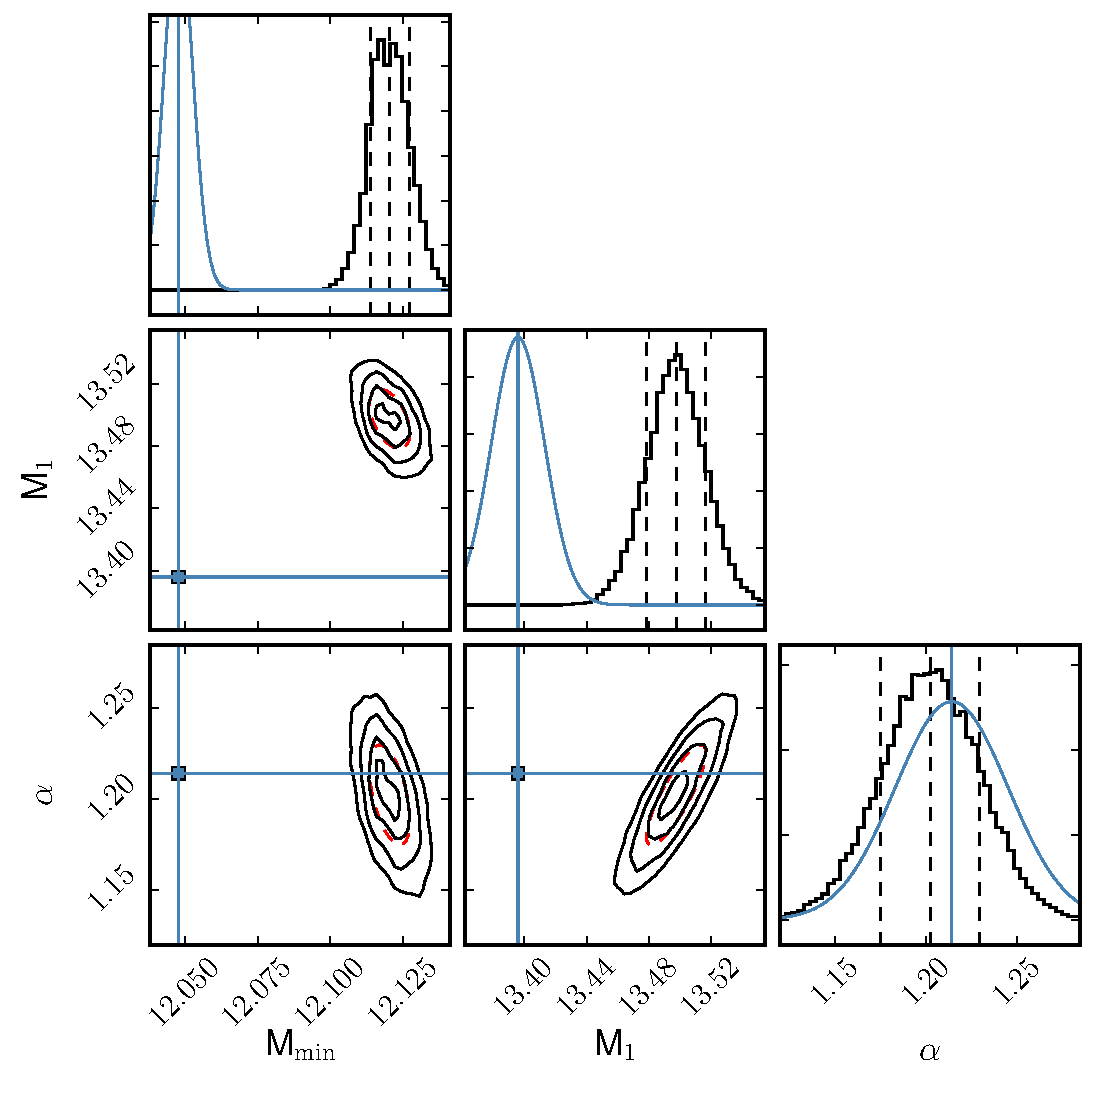
\includegraphics[width=\linewidth]{figures/typical_triangle.pdf} 
% \caption[Marginalised Joint-posteriors for the ``basic" run]{Marginalised joint-posteriors for the basic run, emulating the analysis of B13. Black histograms show the marginalised 1D posterior on each parameter, while black contours show the 2D joint-posteriors, smoothed with a Gaussian KDE. Red dashed contours indicate the 1-$\sigma$ region, when approximated by a bivariate Gaussian distribution, and should correspond to the second black contour perfectly if the true posterior is Gaussian. Blue lines and curves correspond to the result of B13 (the curves show the posterior approximated as a Gaussian).}
% \label{fig:typical}
% \end{figure}

%  \begin{figure}
% \centering
% 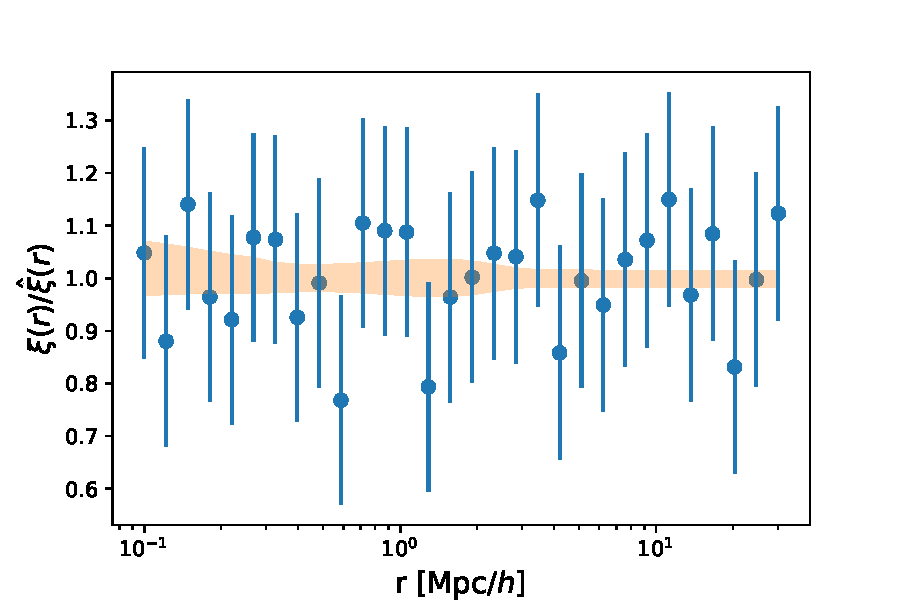
\includegraphics[width=\linewidth]{figures/residuals.pdf} 
% \caption[Residuals for all fits in example application]{Residuals of all our fits. Data from B13 is shown as blue square markers with errorbars. Each of the fits is shown in a different colour. The only fit that is poor in general is that which had a uniformly varied cosmology. This is probably due to the way in which the `best' fit was chosen: as the mean.}
% \label{fig:residuals}
% \end{figure}

% It is well-known that degeneracies between HOD and cosmology parameters prohibit constraints on the latter using only galaxy clustering. We explore this effect in figures \ref{fig:with_cosmo_flat} and \ref{fig:with_cosmo_cov}, which show the marginalised joint-posterior for a similar run, but including five cosmological parameters: $\sigma_8$, $\Omega_m$, $\Omega_b$, $H_0$ and $n_s$. In figure \ref{fig:with_cosmo_flat}, we leave these parameters to vary with a uniform prior, whereas in figure \ref{fig:with_cosmo_cov} they assume their prior from the covariance matrix of P15. Here, the blue lines in the HOD parameter panels are the results from the pure-HOD analysis, and the blue lines in the cosmology panels represent the best-fit P15 values.

% We first note that uniform priors on the cosmology lead to virtually completely unconstrained values (within their ranges), which is in agreement with our expectation. Furthermore, while the HOD values are consistent with their estimated values with a fiducial cosmology, the uncertainties grow considerably (especially in the mass scale parameters), and the distributions are highly non-Gaussian. The latter is most likely due to the effects of the truncated posteriors of the cosmology. 

% When using covariant priors given by the P15 constraints, we find again that the 2PCF is not effective at constraining the cosmology, with the posteriors dominated by the priors. We do however find that the uncertainties on the HOD parameters are increased. In particular, the uncertainty on $M_\text{min}$ is approximately doubled. This highlights the need to include all known uncertainties in the analysis, even if they are to be marginalised over. 

%  \begin{figure*}
% \centering
% 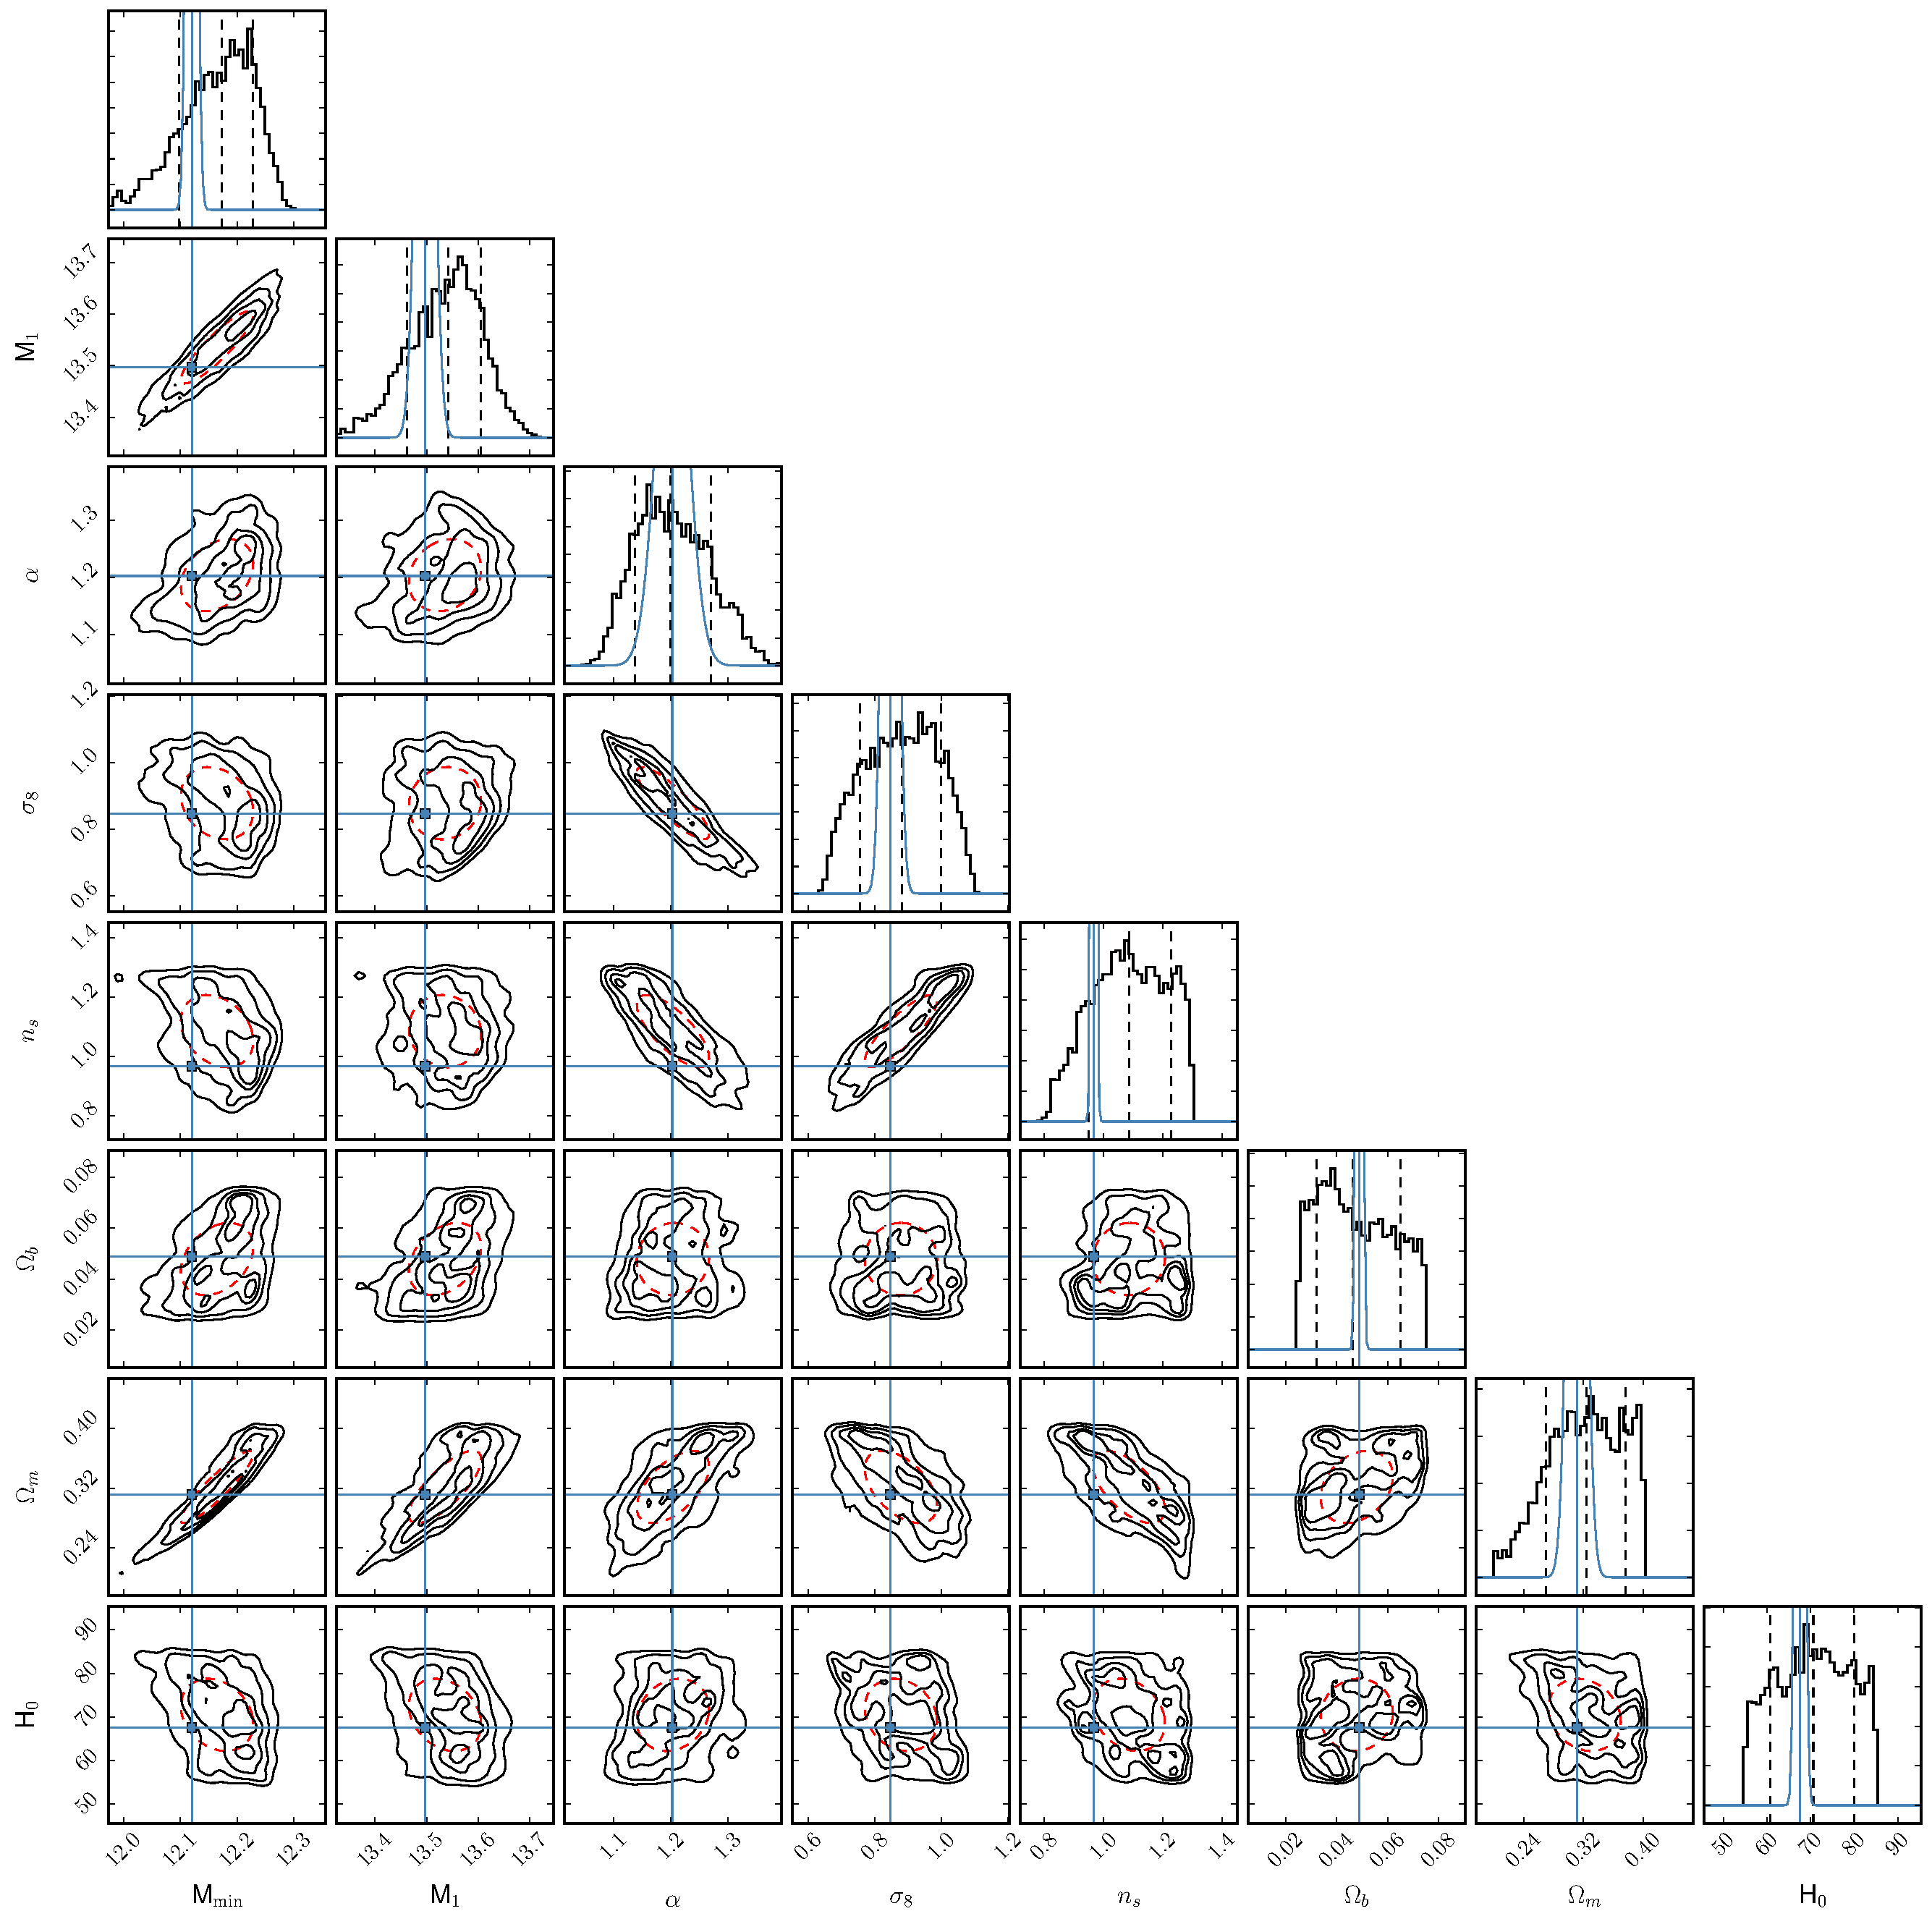
\includegraphics[width=\linewidth]{figures/with_cosmo_flat_triangle.pdf} 
% \caption[Marginalised joint-posteriors for a run with cosmology free to vary with uniform priors]{Marginalised joint-posteriors for a run with cosmology free to vary with uniform priors. The plot is similar to figure \ref{fig:typical}, but in this case, the blue lines/curves correspond to the best-fit HOD-only case (for the HOD parameters) and to the P15 uncertainties (for cosmological parameters). Noticeably, the cosmological parameters are virtually unconstrained.}
% \label{fig:with_cosmo_flat}
% \end{figure*}

%  \begin{figure*}
% \centering
% 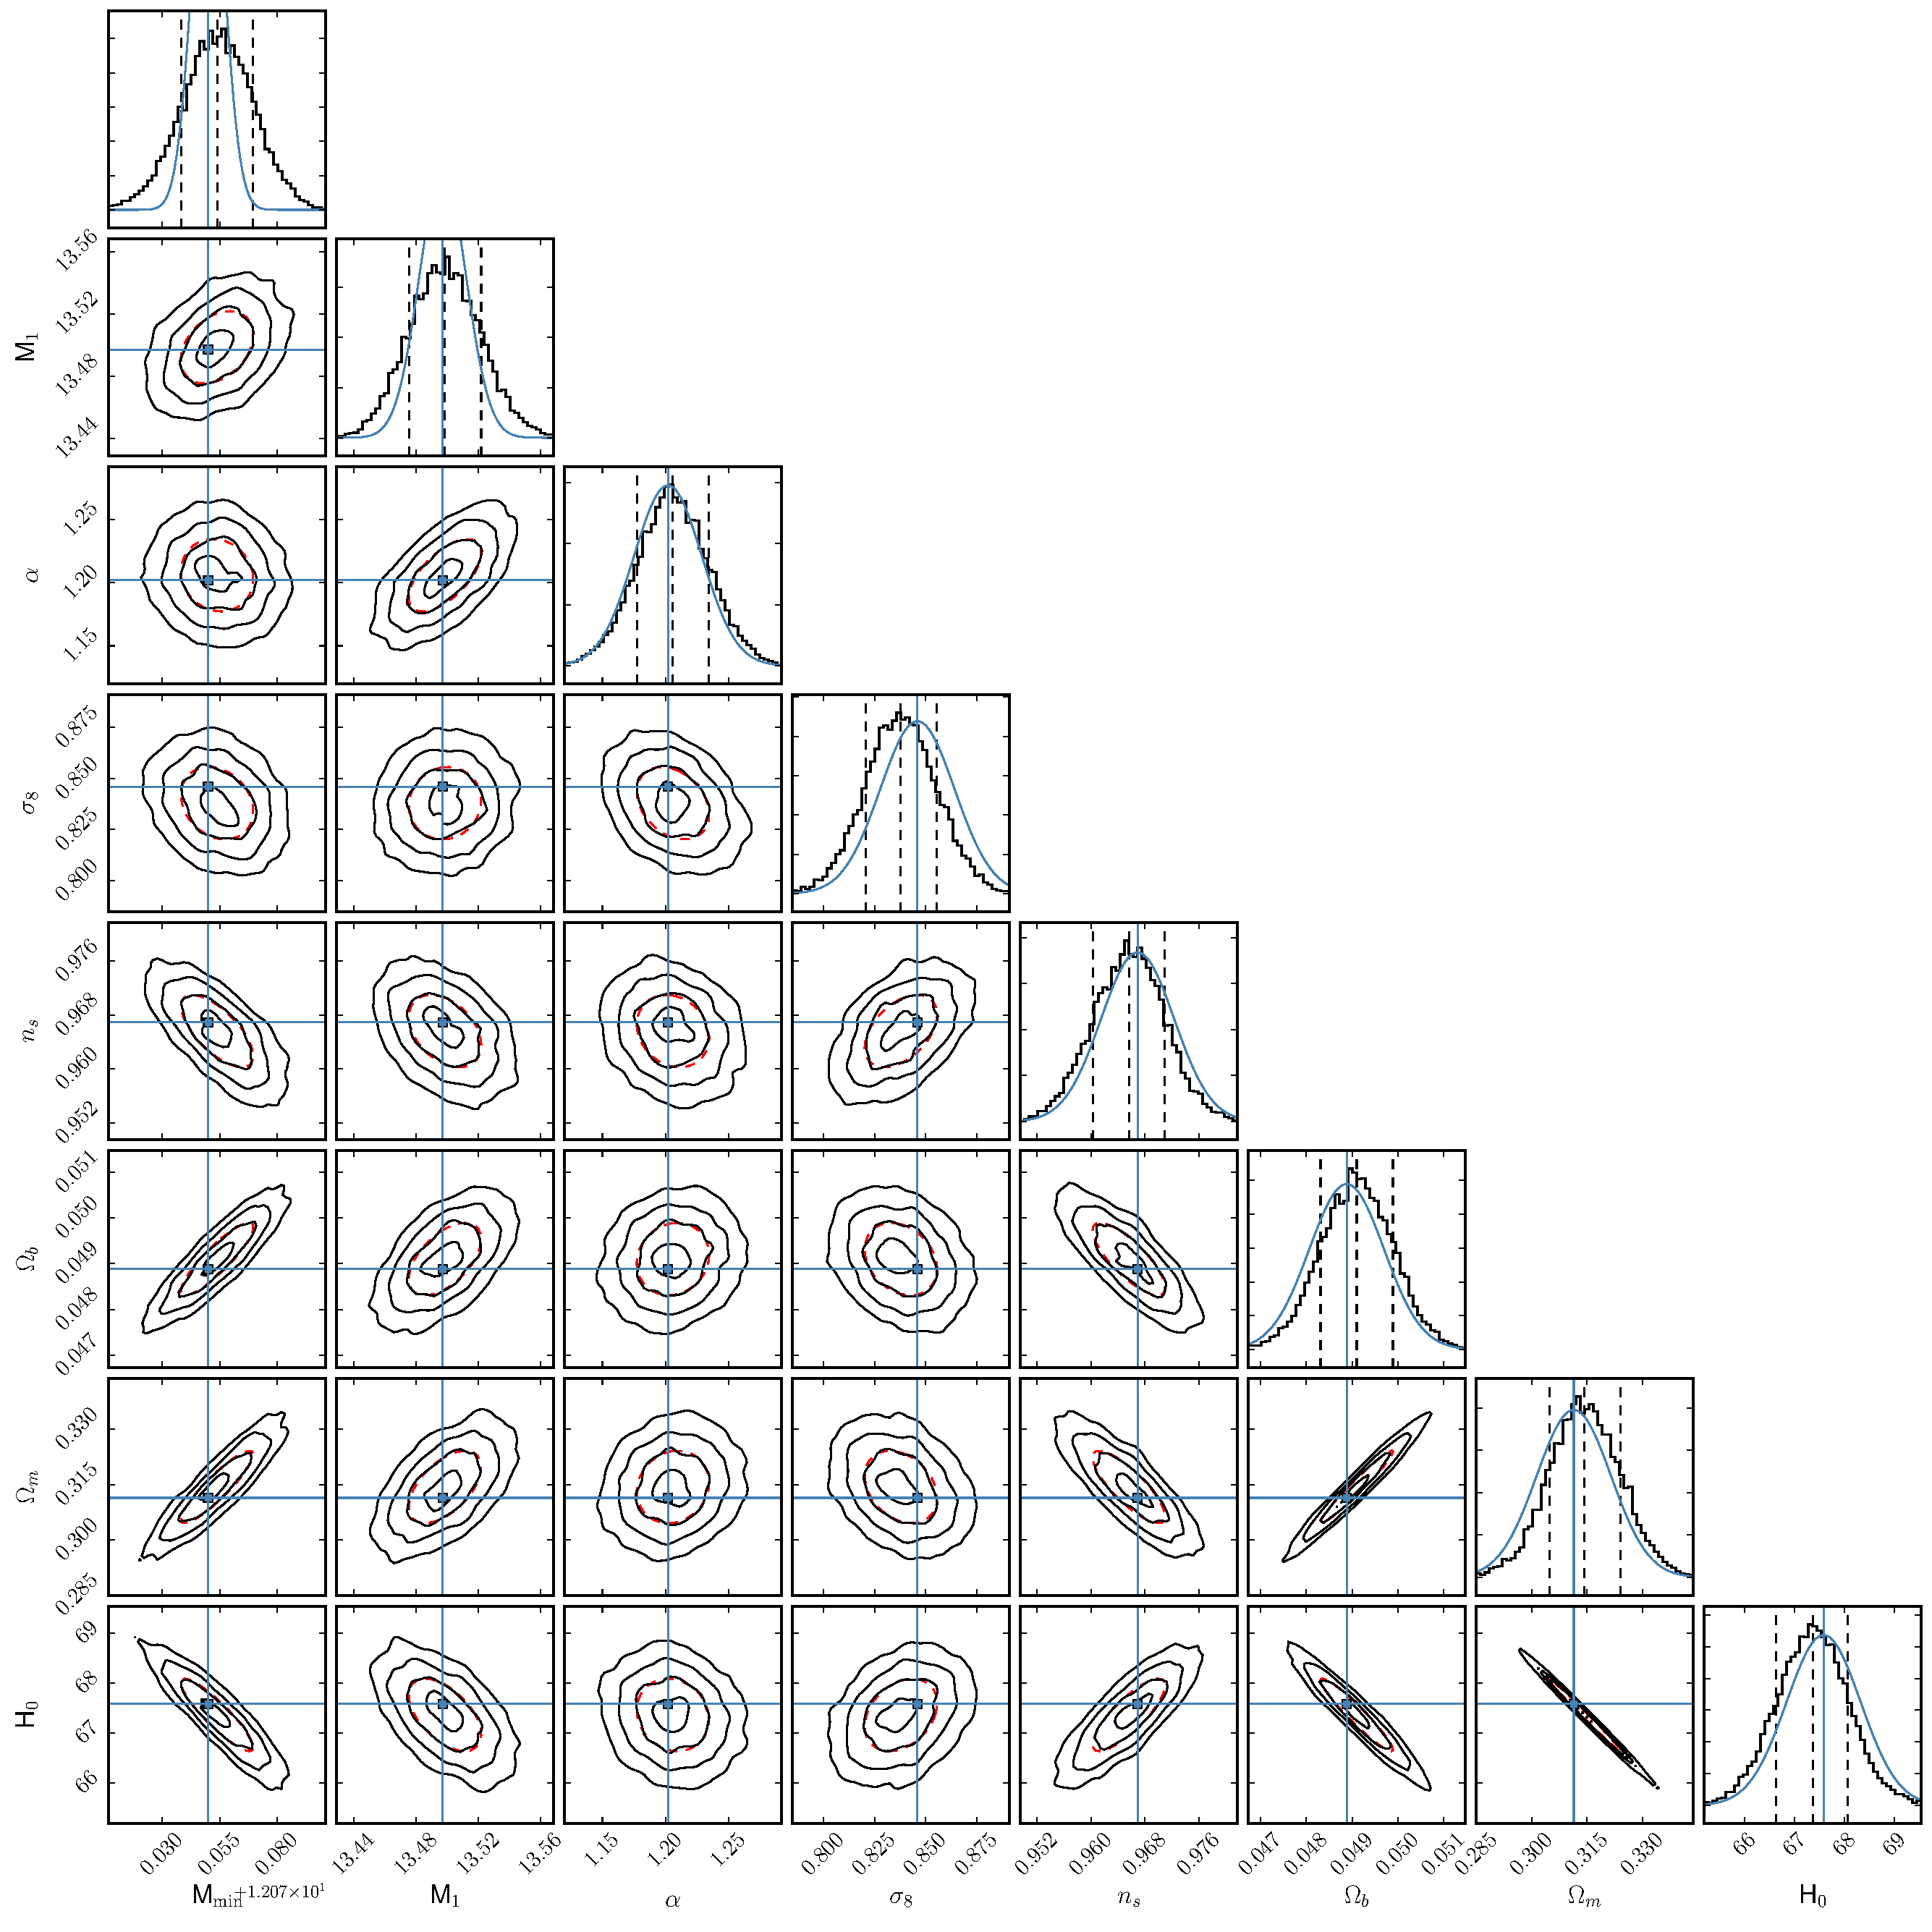
\includegraphics[width=\linewidth]{figures/with_cosmo_cov_triangle.pdf} 
% \caption[Marginalised joint-posteriors for a run with cosmology free to vary with covariant normal priors]{Marginalised joint-posteriors for a run with cosmology free to vary with covariant normal priors. The plot is otherwise precisely the same as figure \ref{fig:with_cosmo_flat}. Cosmological parameters are relatively unchanged, but HOD parameters have looser constraints than when cosmology is fixed.}
% \label{fig:with_cosmo_cov}
% \end{figure*}

% Of course, including known uncertainties in the cosmological parameters is not the final word. The various components involved in the calculation require fitted parameters, which include some uncertainty. The \halomod\  system makes it possible to easily include these uncertainties, by providing the model parameters as variables in the fit. 

% We take a simplistic approach for illustration and set each model parameter for the HMF, the bias and the concentration to have 10\% uncertainty. We again perform the same analysis, and in figure \ref{fig:nuisance} we plot the final marginalised distributions (without the nuisance parameters from the components and cosmology). In this case, the blue curves represent the distributions derived from the fit with covariant cosmology. We find that again, the best-fit parameters are consistent between analyses, but the estimated uncertainty is increased. Interestingly, again it is primarily in the mass scale parameters that the increase occurs, and predominantly $M_\text{min}$. With the increased uncertainty, the tension between our results and those of B13 is relaxed considerably, with the best-fit $M_\text{min}$ from B13 just outside the 1-$\sigma$ region. 

%  \begin{figure}
% \centering
% 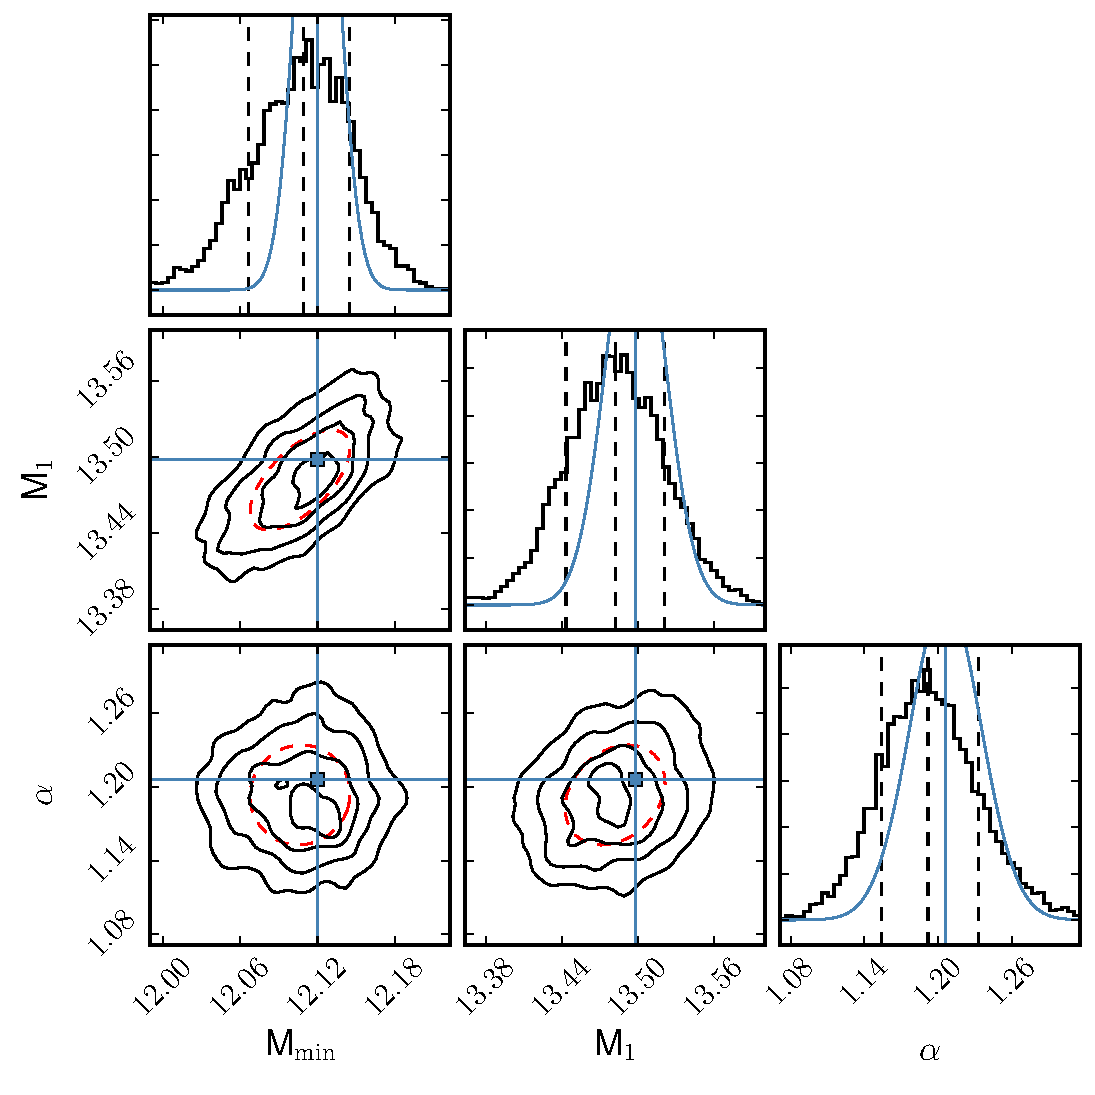
\includegraphics[width=\linewidth]{figures/with_nuisance_triangle.pdf} 
% \caption[Marginalised joint-posteriors for the HOD parameters with the inclusion of both covariant cosmology and nuisance parameters from the HMF, bias and concentration]{Marginalised joint-posteriors for the HOD parameters with the inclusion of both covariant cosmology and nuisance parameters from the HMF, bias and concentration. Blue curves show the distributions derived in the case with covariant cosmology only.}
% \label{fig:nuisance}
% \end{figure}

% Figure \ref{fig:residuals} shows the model calculated from the mean of all the fitted posteriors against the data. Large scales do not contribute significantly to the fit due to the large errors, and so the fits diverge on these scales. Otherwise, the fits are all quite good except for that with a uniformly varying cosmology. 

\section{Future Development}
\label{sec:future}
The current implementation of \textsc{halomod} (likewise \textsc{hmf}) forms a solid framework for evaluating halo model quantities. Its flexible and extendable architecture enables user-side development with updated components and paradigms (eg. warm dark matter, or alternate dark energy scenarios). However, several features considered for future versions are worth mentioning:

\paragraph*{Additional and higher-order statistics}
Though the most popular usage of the halo model has been to analyse the two-point clustering of galaxies, there has also been a range of studies with other quantities. In particular, galaxy-galaxy weak lensing, as an independent observable, has been shown to be able to break HOD degeneracies \citep{Leauthaud2012}. Future versions of \halomod\  will include these quantities in addition to higher-order statistics such as the bispectrum and 3-point correlation function. 

\paragraph*{Alternative Cosmologies}
As already mentioned, \hmf\ already has the infrastructure to support alternative cosmological scenarios. However, only one scenario is actually fleshed out -- WDM. It will be interesting to implement more exotic models such as Early Dark Energy, or $f(R)$ gravity. Ideally, such implementations will arise from the community.

\paragraph*{Support for \textsc{class}}
\textsc{class}\footnote{\url{https://lesgourg.github.io/class_public/class.html}} \citep{Lesgourgues2011} is a popular Boltzmann-solver for the transfer function. As such, it is a prime candidate as an extra model for the \verb|Transfer| \component.

\paragraph*{Performance and Accuracy Improvements}
There are known bottlenecks in the code -- especially as related to Hankel transforms and halo exclusion -- both in memory and CPU. 
These do not affect the user experience greatly over a single model, but make a definite impact when running many models. Further improvements in the interpolation and integration required for Hankel transforms will be highly useful. Reducing the number of nodes required for these integrals will also lower the burden of halo exclusion.

\paragraph*{Improved Web Interface}
Though \thm\ has a clean and usable interface, it was designed and implemented by a definite non-expert in the field of web development. 
Many advanced features that would enhance the user experience are possible: from fitting more useful information into a one-page app, to making the figure(s) interactive, to having the ability to store ``sessions'' for later use. 


Most importantly, \hmf, \halomod\ and \thm\ are all open-source and intended to be projects nurtured and maintained by the community. 
This will make them of more impact and usefulness for the community.
Up-to-date planned improvements for all of these codes can be found by browsing their issues on GitHub\footnote{Eg. \url{https://github.com/steven-murray/halomod/issues}}. We highly encourage the reader to suggest new features via this mechanism!


\section{Summary}
\label{sec:summary}
We have presented a new code, \halomod, accompanied by a web-application, \thm, for the calculation of quantities within the halo model framework. This code aims to satisfy six principles: simple, intuitive, flexible/extendible, comprehensive, efficient and open; we have shown how these criteria have shaped the architecture of the library.

\halomod\  is designed to be a valuable resource for the community. 
To this end, we have presented an illustrative application which helps to get a flavour of how \halomod\ may used `in the wild' for constraining physical parameters using galaxy surveys.

We expect \thm\ to be useful for both theorists and observers, but are especially excited about the prospects for using it educationally. 
\thm\ also serves as an example and motivation for other broadly-applicable codes to make use of scientific web-applications in order to reach a wider user-base.

\section*{Acknowledgements}
SGM acknowledges many useful discussions with colleagues that formed the basis of this paper, including Chris Power, Aaron Robotham, Chris Blake, Florian Beutler and David Palomara. 
All figures in this paper were produced with \textsc{matplotlib} \citep{Hunter2007}. We acknowledge the extremely helpful \textsc{numpy} \citep{vanderWalt2011}, \textsc{astropy} \citep{Robitaille2013,AstropyCollaboration2018} and \textsc{SciPy} \citep{Virtanen2020} codes.


\bibliography{library}

\appendix

\section{\textsc{halomod}'s Caching System}
\label{app:caching}

The \textsc{hmf} package has always included some form of caching, whereby derived quantities are stored for later retrieval, and only updated when absolutely necessary. At the time of its initial publication, \textsc{hmf} relied on each parameter being hard-coded into an \verb|update| method in a specific way so as to trigger re-calculation of all child properties. This required great care when modifying the code, and especially when adding new parameters, as breaking the chain of dependencies could cause subtle errors. 

We have since updated the caching system of \textsc{hmf} to be much more robust. We use Python's function decorators, a kind of functional programming technology, to abstract the caching logic from the main \framework. There is now a specific module containing two methods and a single base class which contain all the machinery for the cache system. This increases the readability of the main code, and maximises the usage of the DRY (Don't Repeat Yourself) principle. 

The caching system makes heavy use of the general distinction between a \parameter\ and \cached. All parameters receive a \verb|@parameter| decorator, which uses function closure to modify its behaviour. Likewise, all quantities receive a \verb|@cached_quantity| decorator.
Every time a \parameter\ or \cached\ is accessed, though it may seem that a simple attribute is being returned, an entire wrapping function is called (though it is built to add very little overhead).

The \verb|@cached_property| decorator performs several operations each time its function is called. Firstly, it is useful to understand that four private tables are stored on the \framework. There are two dictionaries which map parameter names to quantities they affect and vice versa (call these \verb|par_prop| and \verb|prop_par| respectively), a dynamic list of quantities that are \textit{currently being evaluated} called \verb|activeq| (there can be more than one because quantities can be nested), and a simple dictionary mapping quantities to a boolean value which specifies whether it needs to be recalculated, called \verb|recalc|.

The first thing required when accessing a quantity is to update any other active quantities' \verb|prop_par| dictionaries with its own parameter dependencies. This will only do anything if this particular quantity has already been calculated and cached (and thus we know its parameter dependencies). 
Following this, if the quantity is in \verb|recalc| and it doesn't need to be recalculated, just return the cached value.
Otherwise, if it's in \verb|recalc| and \textit{does} need to be recalculated, call the the evaluation function, cache it, switch \verb|recalc| to false for this parameter, and return.
Finally, if it's not in \verb|recalc| at all, this must be the first time we've ever tried to access this quantity. In this case, we first add it to the \verb|activeq|, so that any parameters used while trying to evaluate this quantity will be added to its dependents (in \verb|prop_par|). 
We then evaluate the function and cache it, then invert the (now full) \verb|prop_par| dictionary to obtain \verb|par_prop|. We then remove it from the \verb|activeq| and set its value in \verb|recalc| to false so it isn't recalculated next time, and then return the value.

The missing ingredient to this is how accessing the \texttt{parameter}s adds itself to the \verb|prop_par| of all quantities in \verb|activeq|. This is of course achieved
by all \texttt{parameter}s also being Python descriptors (i.e. decorated), and it is simple for the \parameter\ to iterate through the \verb|activeq| list and add itself to each quantity's \verb|prop_par| entry.

This method is as efficient as possible for such a generalised process. No re-calculations are performed unless necessary. However, higher efficiency could be achieved by simply using low-level functions chained together in an appropriate way, storing only the variables that needed storing for a particular application. This is due to the extra memory usage required to store all variables in the caching system, and the minimal overhead of re-checking the cache. 

Importantly, this process is completely transparent to the user, who merely accesses quantities as if they were pre-stored variables. Furthermore, it is simple for the developer, who merely needs to attach a \verb|@parameter| or \verb|@cached_quantity| to any new parameters or quantities they define. 
\section{Hankel Transform}
 \label{app:hankel}

The transformation from 3D power spectrum to real-space correlation function is given by Eq. \ref{eq:hankel}, and is a zeroth-order spherical Hankel transformation.
It is necessary to perform this transformation to calculate the two-halo correlations, and also for the one-halo term if an analytic form for the self-convolution of the density profile does not exist. 

The transformation poses a challenge \citep[eg.][]{Diemer2018}, as it is highly oscillatory in log-space, in which it is necessary to perform the integration.

\verb|halomod| largely avoids this issue by using a technique outlined in \cite{Szapudi2005}, developed in \cite{Ogata2005}, and implemented in \cite{Murray2019}. 
The technique uses a quadrature rule based on the roots of the Bessel function and a double-exponential transformation. 

The general rule is defined as
\begin{equation}
	\label{eq:hankeltrans}
	\int_0^\infty f(x)J_\nu(x) dx \approx \pi \sum_{k=1}^\infty w_{\nu k} f(y_{\nu k})J_\nu(y_{\nu k})\psi'(hr_{\nu k}),
\end{equation}
where $h$ is an integration step-size (similar to the trapezoidal rule) and
\begin{eqnarray}
	y_{\nu k} &=& \pi \psi(hr_{\nu k})/h \\
	\psi(t) &=& t\tanh(\pi \sinh(t)/2) \\
	\psi'(t) &=& \frac{\pi t \cosh(t) + \sinh(\pi \sinh(t))}{ 1 + \cosh(\pi \sinh(t))} \\
	w_{\nu k} &=& \frac{Y_\nu(\pi r_{\nu k})}{J_{\nu+1}(\pi r_{\nu k})}.
\end{eqnarray}
Here $J_\nu(x)$ represents a Bessel function of the first kind of order $\nu$, and $Y_\nu(x)$ a Bessel function of the second kind. Lastly, $r_{\nu k}$ are the roots of the Bessel function $J_\nu$, divided by $\pi$ (alternatively, the roots of $J_\nu(\pi x)$).

In the case of the zeroth-order spherical Hankel transform, we may make some simplifications. We firstly take Eq. \ref{eq:hankel} and make the substitution $z=kr$:
\begin{equation}
	\label{eq:hankelsub}
	\xi(r) = \frac{1}{2\pi^2r^3}\int_0^\infty P(z/r)z^2j_0(z)dz,
\end{equation} 
where $j_0$ is the spherical Bessel function of order zero. We also note that the spherical Bessel functions are related to the standard functions by
\begin{equation}
	\label{eq:sphbessel}
	j_\nu(x) = \sqrt{\frac{\pi}{2x}}J_{\nu+1/2}(x),
\end{equation}
so we may update Eq. \ref{eq:hankelsub} to
\begin{equation}
	\label{eq:finalhankel}
	\xi(r) = \frac{1}{2\pi^2r^3}\int_0^\infty P(z/r) z^2\sqrt{\frac{\pi}{2z}}J_{1/2}(z)dz.
\end{equation}
Eq. \ref{eq:finalhankel} is in the form required to implement the method of \cite{Ogata2005}, with $\nu=1/2$. In this case, the zeros of the function, $r_{\nu k} = 1,2,3...$. 

We may make one further optimization by noticing that 
\begin{equation}
	\label{eq:weq1}
	w_{1/2 k} = \frac{y_0(x_k)}{j_1(x_k)} = \frac{-\cos(x_k)/x_k}{\sin(x_k)/x_k^2 - \cos(x_k)/x_k} = 1,
\end{equation}
where the last equality holds because $x_k = \pi r_{1/2,k}$ are defined as the roots of $\sin(x)$.
Thus we finally arrive at the equation
\begin{equation}
	\label{eq:hankel_final_identity}
	\xi(r) \approx \pi \sum_{k=1}^\infty f(y_{1/2, k})J_{1/2}(y_{1/2, k})\psi'(hr_{1/2, k}),
\end{equation}
with
\begin{equation}
	\label{eq:f}
	f(x) = P(x/r)x^2\sqrt{\frac{\pi}{2x}}.
\end{equation}

In practice, the infinite sum is truncated at some finite value $N$. 
The benefit of this method, due to the double-exponential transformation, is that this $N$ can be quite small for a very accurate result. 
Since the values, $y_{\nu k}$, at which the sum is evaluated approach the zeros of the bessel function as $k \rightarrow 0$, \citet{Murray2019} found that a maximum of $N=3.2/h$ steps are required (for reasonably small $h$).

 The required value of $h$ is mostly dictated by the existence of information in the integrand at low $x$. As expected, a smaller value of $h$ will in general give more accurate results (modulo accumulated numerical addition error). The requisite value of $h$ will be different when transforming 
 different functions. 
 %In particular, when transforming $P(k)$ to $\xi(r)$, the low-$k$ convergence of $P(k)$ towards zero makes it possible to use higher $h$.
 
 To avoid potential memory issues, we sum Eq. \ref{eq:hankel_final_identity} in chunks of 100 terms, checking for convergence after each chunk.
 We find in general that using $h=0.005$ for the $P(k) \rightarrow \xi(r)$ transformation is sufficient. 
 
 A consistent way to test the accuracy of the transform is to perform a full round-trip transform from $P(k) \rightarrow \xi(r) \rightarrow P(k)$ and check whether the result is close to the input.
 Since the transform uses values of $f(x)$ for $x$ as small as $\sim 10h$ and as large as $\sim 10/h$, corresponding to $k$ values between $(10 h / r_{\rm max}, 10/(h r_{\rm min})$ (and similarly for $r$),
 the vectorized $P(k_i)$ and $\xi(r_i)$ need to be extrapolated -- a procedure that must be done carefully, but will still yield some error for points outside the original domain.
 Thus the accuracy of the round-trip transform fundamentally depends on the choice of $r$-vector: $r_{\rm min}$, $r_{\rm max}$ and $d\log r$, as well as $h_k$ and $h_r$ (the resolution of the integration in the forward and backwards transforms). 
 We find that for the linear power spectrum, we achieve an error of less than 1\% over scales $k \in (10^{-2}, 10^4)$ using the parameters $r_{\rm min} = 10^{-3}$, $r_{\rm max} = 10^{3.5}$, $d\log r = 0.01$, $h_k = 10^{-4}$ and $h_r = 10^{-3}$.
 
 For scales $k < 10^{-2}$, the 2-halo term may be very well approximated by the linear power multiplied by the effective bias (Eq. \ref{eq:beff}), and we switch to that approximation on these scales (otherwise $r_{\rm max}$ would need to grow significantly, reducing performance).
 

\section{Projected Correlation Function Limits}
\label{app:proj}
The finite upper limit can be handled empirically, keeping in mind that the correlation function may become negative at large scales (to a small degree). 
To perform this convergence test, we cumulatively integrate the real-space correlation function at several scales $r_p$, determining where the contribution to the integral becomes less than a percent. 
While there is no continuous relation which describes this location as a function of $r_p$, we deduce the following stepwise prescription:
\begin{equation}
	r_{\rm max} = {\rm max}(80.5,5r_p).
\end{equation}
This prescription captures the idea that for small $r_p$, we do not want to integrate out to negative correlation, while for larger $r_p$, we must integrate well past the point at which the correlation becomes negative. In practice, measurements of the projected correlation function usually set a finite upper limit of $\sim 60 h^{-1}$Mpc, and we allow the user to set this arbitrarily if desired.

The finite lower limit has more difficult convergence properties. We make the substitution $y=r-r_p$ in Eq. \ref{eq:wprp} and multiply by $y$ to estimate the contribution of each (logarithmic) scale to the integral. We then proceed to perform an approximate analytic analysis of the convergence by assuming that as $y \rightarrow 0$, the correlation can be expressed as a power law $\xi(r) \approx r^{-a}$. This yields the following expression for the contribution of each scale $r$:
 \begin{equation}
 	\label{eq:projcorrcontr}
 	C(y,a,r_p) = \frac{y(y+r_p)^{(1-a)}}{\sqrt{y(y+2r_p)}}.
 \end{equation} 

This equation shows a characteristic shape, with a peak around the scale $r_p$. 
This indicates that the integral limit must be less than the scale of this peak.
In fact, we deduce the scale at which the contribution is 1\% of the value at the peak, to ensure sub-percent accuracy.

To do this, we solve $d C(y,a,r_p)/dy = 0$ for $y=r_{\rm peak}$, and calculate $C(r_{\rm peak},a,r_p) = C_{\rm max}$. The next step is to solve $C(y,a,r_p) = f_{\rm peak}C_{\rm max}$, where $f_{\rm peak}$ is the fraction of the peak value we wish to locate (we set this to 0.01 in our implementation). However this is not analytically solvable. We make the valid assumption that at the solution, $y \ll r_p$ (since the peak is around $r_p$). 
This enables us to solve the simple equation 
\begin{equation}
	\label{eq:projcorrsolve}
	r_p^{1-a}\sqrt{y_{\rm cut}/(2r_p)} = f_{\rm peak}C_{\rm max},
\end{equation}
which has the solution
\begin{equation}
	\label{eq:projcorrsolution}
	y_{\rm cut} = \theta(a)r_pf_{\rm peak}^2,
\end{equation}
where
\begin{align}
	\label{eq:theta}
	\theta(a) &= \frac{-2 a^3+\left(p+9\right) a^2-\left(3p+13\right) a+3p+7}{2(a-1)^2 \left[p+22(a-1)\right]\left(\frac{p+1}{a-1}\right)^{2 a}} \\
	p &= \sqrt{4 a^2-8 a+5}
\end{align}

$\theta(a)$ is a weakly but monotonically decreasing function, of the order $\approx 0.1$ in the range of $a$ we are interested in. In \verb|halomod|, $y_{\rm cut}$ is calculated for each $r_p$, ensuring accuracy at any scale.

\end{document}